% Options for packages loaded elsewhere
\PassOptionsToPackage{unicode}{hyperref}
\PassOptionsToPackage{hyphens}{url}
%
\documentclass[
]{book}
\usepackage{amsmath,amssymb}
\usepackage{lmodern}
\usepackage{iftex}
\ifPDFTeX
  \usepackage[T1]{fontenc}
  \usepackage[utf8]{inputenc}
  \usepackage{textcomp} % provide euro and other symbols
\else % if luatex or xetex
  \usepackage{unicode-math}
  \defaultfontfeatures{Scale=MatchLowercase}
  \defaultfontfeatures[\rmfamily]{Ligatures=TeX,Scale=1}
\fi
% Use upquote if available, for straight quotes in verbatim environments
\IfFileExists{upquote.sty}{\usepackage{upquote}}{}
\IfFileExists{microtype.sty}{% use microtype if available
  \usepackage[]{microtype}
  \UseMicrotypeSet[protrusion]{basicmath} % disable protrusion for tt fonts
}{}
\makeatletter
\@ifundefined{KOMAClassName}{% if non-KOMA class
  \IfFileExists{parskip.sty}{%
    \usepackage{parskip}
  }{% else
    \setlength{\parindent}{0pt}
    \setlength{\parskip}{6pt plus 2pt minus 1pt}}
}{% if KOMA class
  \KOMAoptions{parskip=half}}
\makeatother
\usepackage{xcolor}
\IfFileExists{xurl.sty}{\usepackage{xurl}}{} % add URL line breaks if available
\IfFileExists{bookmark.sty}{\usepackage{bookmark}}{\usepackage{hyperref}}
\hypersetup{
  pdftitle={LECTURE NOTES OF STAT 3202},
  pdfauthor={Dr.~Pratheesh P. Gopinath},
  hidelinks,
  pdfcreator={LaTeX via pandoc}}
\urlstyle{same} % disable monospaced font for URLs
\usepackage{longtable,booktabs,array}
\usepackage{calc} % for calculating minipage widths
% Correct order of tables after \paragraph or \subparagraph
\usepackage{etoolbox}
\makeatletter
\patchcmd\longtable{\par}{\if@noskipsec\mbox{}\fi\par}{}{}
\makeatother
% Allow footnotes in longtable head/foot
\IfFileExists{footnotehyper.sty}{\usepackage{footnotehyper}}{\usepackage{footnote}}
\makesavenoteenv{longtable}
\usepackage{graphicx}
\makeatletter
\def\maxwidth{\ifdim\Gin@nat@width>\linewidth\linewidth\else\Gin@nat@width\fi}
\def\maxheight{\ifdim\Gin@nat@height>\textheight\textheight\else\Gin@nat@height\fi}
\makeatother
% Scale images if necessary, so that they will not overflow the page
% margins by default, and it is still possible to overwrite the defaults
% using explicit options in \includegraphics[width, height, ...]{}
\setkeys{Gin}{width=\maxwidth,height=\maxheight,keepaspectratio}
% Set default figure placement to htbp
\makeatletter
\def\fps@figure{htbp}
\makeatother
\setlength{\emergencystretch}{3em} % prevent overfull lines
\providecommand{\tightlist}{%
  \setlength{\itemsep}{0pt}\setlength{\parskip}{0pt}}
\setcounter{secnumdepth}{5}
\usepackage{booktabs}
\AtBeginDocument{\renewcommand{\chaptername}{}}  
\usepackage{booktabs}
\usepackage{longtable}
\usepackage{array}
\usepackage{multirow}
\usepackage{wrapfig}
\usepackage{float}
\usepackage{colortbl}
\usepackage{pdflscape}
\usepackage{tabu}
\usepackage{threeparttable}
\usepackage{threeparttablex}
\usepackage[normalem]{ulem}
\usepackage{makecell}
\usepackage{xcolor}
\ifLuaTeX
  \usepackage{selnolig}  % disable illegal ligatures
\fi
\usepackage[]{natbib}
\bibliographystyle{apalike}

\title{LECTURE NOTES OF STAT 3202}
\author{Dr.~Pratheesh P. Gopinath}
\date{2022-01-30}

\begin{document}
\maketitle

{
\setcounter{tocdepth}{1}
\tableofcontents
}
\hypertarget{welcome}{%
\chapter*{Welcome}\label{welcome}}
\addcontentsline{toc}{chapter}{Welcome}

Welcome to the book \textbf{LECTURE NOTES ON STATISTICAL METHODS AND APPLICATIONS}.

\hypertarget{preface}{%
\chapter*{Preface}\label{preface}}
\addcontentsline{toc}{chapter}{Preface}

\textbf{Note}: This book is published in MeLoN (Module for e-Learning \& Online Notes) . The online version of this book is free to read here.

If you have any feedback, please feel free to contact \href{https://coavellayani.kau.in/people/dr-pratheesh-p-gopinath}{Dr.Pratheesh P. Gopinath}. E-mail: \texttt{pratheesh.pg@kau.in} Thank you!

This book is a collection of all lecture notes covering the syllabus of statistics course in B.Sc.(Hons.) Agriculture under Kerala Agricultural University

\begin{center}
\includegraphics[width=0.3\linewidth]{docs/logo} \end{center}

\hypertarget{introduction}{%
\chapter{Introduction}\label{introduction}}

In this lecture we will have the introduction, which includes, definition of statistics, collection and classification of data, formation of frequency distribution.\citep{goon} \citep{gupta}

\hypertarget{origin-of-the-word-statistics}{%
\section{Origin of the word ``Statistics''}\label{origin-of-the-word-statistics}}

The term statistics was derived from the Neo-Latin word \texttt{statisticum\ collegium} meaning ``council of state'' and the Italian word \texttt{statista} meaning ``statesman'' or ``politician''.

A German word \texttt{Statistik}, got the meaning ``collection and classification of data'' generally in the early 19th century. This word was first introduced by Gottfried Achenwall (1749). \texttt{Statistik} was originally designated as a term for analysis of data about the state (data used by government or other administrative bodies). The term \texttt{Statistik} was introduced into English in 1791 by Sir John Sinclair when he published the first of 21 volumes titled ``Statistical Account of Scotland'' \citep{ball}. The first book to have `Statistics' in its title was ``Contributions to Vital Statistics'' (1845) by Francis GP Neison, actuary\footnote{actuary: A person who compiles and analyses statistics and uses them to calculate insurance risks and premiums.} to the Medical Invalid and General Life Office.

\begin{figure}

{\centering 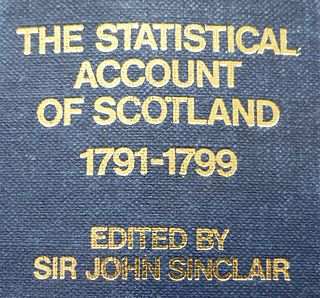
\includegraphics[width=4.44in]{images/history1} 

}

\caption{Statistical Account of Scotland by Sir John Sinclair (1791)}\label{fig:scotland}
\end{figure}

\hypertarget{statistics-and-mathematics}{%
\section{Statistics and Mathematics}\label{statistics-and-mathematics}}

Mathematics follows a rigid theorem and proof. Mathematical theories involve well-defined and proven facts which has the minimal scope of change. However, Statistics is a discipline where real-life data is handled. This factor makes this field of study more abstract, where individuals have to develop newer solutions to problems that was new and not observed before. Statistics is an applied science; in mathematics the goal is to prove theorems. In statistics, the main goal is to develop good methods for understanding data and making decisions. Statisticians often use mathematical theorems to justify their methods, but theorems are not the main focus. Statistics is now considered as an independent field which uses mathematics to solve real life problems.

\hypertarget{definition-of-statistics}{%
\section{Definition of Statistics}\label{definition-of-statistics}}

Statistics is the science which deals with the

\begin{itemize}
\item
  Collection of data
\item
  Organization of data or Classification of data
\item
  Presentation of data
\item
  Analysis of data
\item
  Interpretation of data
\end{itemize}

Two main branches of statistics are:

\textbf{Descriptive statistics}, which deals with summarizing data from a sample using indexes such as the mean or standard deviation etc.

\textbf{Inferential statistics}, use a random sample of data taken from a population to describe and make inferences about the population parameters.

\hypertarget{data}{%
\section{Data}\label{data}}

Data can be defined as individual pieces of factual information recorded and used for the purpose of analysis. It is the raw information from which inferences are drawn using the science ``STATISTICS''.

Example for data

\begin{itemize}
\item
  No.~of farmers in a block.
\item
  The rainfall over a period of time.
\item
  Area under paddy crop in a state.
\end{itemize}

\hypertarget{use-and-limitations-of-statistics}{%
\section{Use and limitations of statistics}\label{use-and-limitations-of-statistics}}

\textbf{Functions of statistics}: Statistics simplifies complexity, presents facts in a definite form, helps in formulation of suitable policies, facilitates comparison and helps in forecasting. Valid results and conclusion are obtained in research experiments using proper statistical tools.

\textbf{Uses of statistics:} Statistics has pervaded almost all spheres of human activities. Statistics is useful in the administration, Industry, business, economics, research workers, banking,insurance companies etc.

\textbf{Limitations of Statistics}

\begin{itemize}
\item
  Statistical theories can be applied only when there is variability in the experimental material.
\item
  Statistics deals with only aggregates or groups and not with individual objects.
\item
  Statistical results are not exact.
\item
  Statistics are often misused.
\end{itemize}

\hypertarget{population-and-sample}{%
\section{Population and Sample}\label{population-and-sample}}

Consider the following example.Suppose we wish to study the body masses of all students of College of Agriculture, Vellayani. It will take us a long time to measure the body masses of all students of the college and so we may select 20 of the students and measure their body masses (in kg). Suppose we obtain the measurements like this

49 56 48 61 59 43 58 52 64 71 57 52 63 58 51 47 57 46 53 59

In this study, we are interested in the body masses of all students of College of Agriculture, Vellayani. The set of body masses of all students of College of Agriculture, Vellayani is called the \textbf{population} of this study. The set of 20 body masses, \emph{W} = \{49, 56,48, \ldots, 53, 59\}, is a \textbf{sample} from this population.

\hypertarget{population}{%
\subsection{Population}\label{population}}

A population is the set of all objects we wish to study

\hypertarget{sample}{%
\subsection{Sample}\label{sample}}

A sample is part of the population we study to learn about the population.

\hypertarget{variables-and-constants}{%
\section{Variables and constants}\label{variables-and-constants}}

\hypertarget{variables}{%
\subsection{Variables}\label{variables}}

Any type of observation which can take different values for different people, or different values at different times, or places, is called a variable. The following are examples of variables:

\begin{itemize}
\item
  family size, number of hospital beds, number of schools in a country, etc.
\item
  height, mass, blood pressure, temperature, blood glucose level, etc.
\end{itemize}

Broadly speaking, there are two types of variables -- \textbf{quantitative} and \textbf{qualitative} (or categorical) variables

\hypertarget{constants}{%
\subsection{Constants}\label{constants}}

Constants are characteristics that have values that do not change. Examples of constants are: pi (𝝅) = the ratio of the circumference of a circle to its diameter (𝝅 = 3.14159...) and \emph{e}, the base of the natural or (Napierian) logarithms (\emph{e}=2.71828).

\hypertarget{types-of-variables}{%
\section{Types of variables}\label{types-of-variables}}

\hypertarget{quantitative-variables}{%
\subsection{Quantitative variables}\label{quantitative-variables}}

A quantitative variable is one that can take numerical values. The variables like family size, number of hospital beds, number of schools in a country, height, mass, blood pressure, temperature, blood glucose level, etc. are examples of quantitative variables. Quantitative variables may be characterized further as to whether they
are discrete or continuous

\hypertarget{discrete-variables}{%
\subsection{Discrete variables}\label{discrete-variables}}

The variables like family size, number of hospital beds, number of schools in a country, etc. can be counted. These are examples of discrete variables. Variables that can only take on a finite number of values are called "discrete variables." Any variable phrased as ``the number of \ldots{}'', is discrete, because it is possible to list its possible
values \{0,1, \ldots\}. Any variable with a finite number of possible values is discrete. The following example illustrates the point. The number of daily admissions to a hospital is a discrete variable since it can be represented by a whole number, such as 0, 1, 2 or 3. The number of daily
admissions on a given day cannot be a number such as 1.8, 3.96 or 5.33.

\hypertarget{continuous-variables}{%
\subsection{Continuous variables}\label{continuous-variables}}

The variables like height, mass, blood pressure, temperature, blood glucose level, etc. can be measured. These are examples of continuous variables. A continuous variable does not possess the gaps or interruptions characteristic of a discrete variable. A continuous
variable can assume any value within a specific relevant interval of values assumed by the variable. Notice that age is continuous since an individual does not age in discrete jumps. Weight can be measured as 35.5, 35.8 kg etc so, it is a continuous variable.

\hypertarget{categorical-variables}{%
\subsection{Categorical variables}\label{categorical-variables}}

A variable is called categorical when the measurement scale is a set of categories. For example, marital status, with categories (single,married, widowed), is categorical. Whether employed (yes, no), religious affiliation (Protestant, Catholic, Jewish, Muslim, others, none),
colours etc. Categorical variables are often called qualitative. It can be seen that categorical variables can neither be measured nor counted.

\hypertarget{measurement-scales}{%
\section{Measurement scales}\label{measurement-scales}}

Variables can further be classified according to the following four levels of measurement: nominal, ordinal, interval and ratio.

\hypertarget{nominal-scale}{%
\subsection{Nominal scale}\label{nominal-scale}}

This scale of measure applies to qualitative variables only. On the nominal scale, no order is required. For example,gender is nominal, blood group is nominal, and marital status is also nominal. We cannot perform arithmetic operations on data measured on the nominal scale.

\hypertarget{ordinal-scale}{%
\subsection{Ordinal scale}\label{ordinal-scale}}

This scale also applies to qualitative data. On the
ordinal scale, order is necessary. This means that one category is lower than the next one or vice versa. For example, Grades are ordinal, as excellent is higher than very good, which in turn is higher than good, and so on. It should be noted that, in the ordinal scale, differences between category values have no meaning.

\hypertarget{interval-scale}{%
\subsection{Interval scale}\label{interval-scale}}

This scale of measurement applies to quantitative
data only. In this scale, the zero point does not indicate a total absence of the quantity being measured. An example of such a scale is temperature on the Celsius or Fahrenheit scale. Suppose the minimum temperatures of 3 cities, A, B and C, on a particular day were 0\textsuperscript{0}C, 20\textsuperscript{0}C and 10\textsuperscript{0}C, respectively. It is clear that we can find the differences between these temperatures. For example, city B is 20\textsuperscript{0}C hotter than city A. However, we cannot say that city A has no temperature. Moreover, we cannot say that city B is twice as hot as city C, just because city B is 20\textsuperscript{0}C and city C is 10\textsuperscript{0}C. The reason is that, in the interval scale, the ratio between two numbers is not meaningful.

\hypertarget{ratio-scale}{%
\subsection{Ratio scale}\label{ratio-scale}}

This scale of measurement also applies to quantitative
data only and has all the properties of the interval scale. In addition to these properties, the ratio scale has a meaningful zero starting point and a meaningful ratio between 2 numbers. An example of variables measured on the ratio scale, is weight. A weighing scale that reads 0 kg
gives an indication that there is absolutely no weight on it. So the zero starting point is meaningful. If Ram weighs 40 kg and Laxman weighs 20 kg, then Ram weighs twice as Laxman. Another example of a variable measured on the ratio scale is temperature measured on the Kelvin scale. This has a true zero point.

\begin{figure}

{\centering 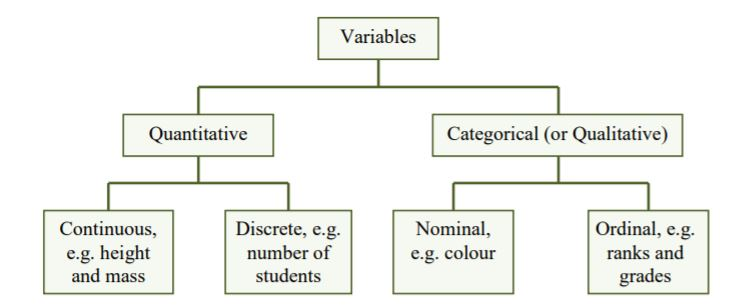
\includegraphics[width=0.7\linewidth]{images/image2} 

}

\caption{Classification of variables}\label{fig:variables}
\end{figure}

\hypertarget{collection-of-data}{%
\section{Collection of Data}\label{collection-of-data}}

The first step in any enquiry (investigation) is the collection of data. The data may be collected for the whole population or for a sample only. It is mostly collected on a sample basis. Collecting data is very difficult job. The enumerator or investigator is the well trained individual who collects the statistical data. The respondents are the persons from whom the information is collected.

\hypertarget{types-of-data}{%
\subsection{Types of Data}\label{types-of-data}}

There are two types (sources) for the collection of data:
* Primary Data\\
* Secondary Data

\hypertarget{primary-data}{%
\subsubsection{Primary Data}\label{primary-data}}

Primary data are the first hand information which is collected, compiled and published by organizations for some purpose. They are the most original data in character and have not undergone any sort of statistical treatment.

Example: Population census reports are primary data because these are collected, complied and published by the population census organization.

\hypertarget{secondary-data}{%
\subsubsection{Secondary Data}\label{secondary-data}}

The secondary data are the second hand information which is already collected by an organization for some purpose and are available for the present study. Secondary data are not pure in character and have undergone some treatment at least once.

Example: An economic survey of England is secondary data because the data are collected by more than one organization like the Bureau of Statistics, Board of Revenue, banks, etc.

\hypertarget{methods-of-collecting-primary-data}{%
\section{Methods of Collecting Primary Data}\label{methods-of-collecting-primary-data}}

Primary data are collected using the following methods:

\hypertarget{personal-investigation}{%
\subsection{Personal Investigation}\label{personal-investigation}}

The researcher conducts the survey him/herself and collects data from it. The data collected in this way are usually accurate and reliable. This method of collecting data is
only applicable in case of small research projects.

\hypertarget{through-investigation}{%
\subsection{Through Investigation}\label{through-investigation}}

Trained investigators are employed to collect the data. These investigators contact the individuals and fill in
questionnaires after asking for the required information. Most organizations utilize this method.

\hypertarget{collection-through-questionnaire}{%
\subsection{Collection through Questionnaire}\label{collection-through-questionnaire}}

Researchers get the data from local representations or agents that are based upon their own experience. This method is quick but gives only a rough estimate.

\hypertarget{through-the-telephone}{%
\subsection{Through the Telephone}\label{through-the-telephone}}

Researchers get information from individuals through the telephone. This method is quick and gives accurate information.

\hypertarget{methods-of-collecting-secondary-data}{%
\section{Methods of Collecting Secondary Data}\label{methods-of-collecting-secondary-data}}

Secondary data are collected by the following methods:

\hypertarget{official}{%
\subsection{Official}\label{official}}

Publications from the Statistical Division, Ministry of Finance, the Federal Bureaus of Statistics, Ministries of Food, Agriculture, Industry, Labor, etc.

\hypertarget{semi-official}{%
\subsection{Semi-Official}\label{semi-official}}

\begin{itemize}
\tightlist
\item
  Publications from State Bank, Railway Board, Central Cotton Committee, Boards of Economic Enquiry etc.\\
\item
  Publication of Trade Associations, Chambers of Commerce, etc.\\
\item
  Technical and Trade Journals and Newspapers.\\
\item
  Research Organizations such as universities and other institutions.
\end{itemize}

\hypertarget{difference-between-primary-and-secondary-data}{%
\section{Difference Between Primary and Secondary Data}\label{difference-between-primary-and-secondary-data}}

The difference between primary and secondary data is only a change of hand. Primary data are the first hand information which is directly collected form one source. They are the most original in character and have not undergone any sort of statistical treatment, while secondary data are obtained from other sources or agencies. They are not pure in character and have undergone some treatment at least once.

\hypertarget{frequency-distribution}{%
\section{Frequency distribution}\label{frequency-distribution}}

Table shows the number of children per family for 54 families selected from a town in India. The data, presented in this form in which it was collected, is called raw data.\\

\begin{figure}

{\centering 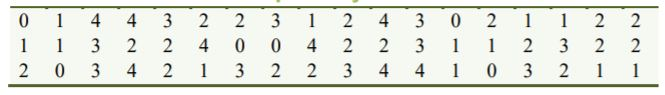
\includegraphics[width=0.7\linewidth]{images/image3} 

}

\caption{raw data set of No. of children in 54 families}\label{fig:raw}
\end{figure}

It can be seen that, the minimum and the maximum numbers of children per family are 0 and 4, respectively. Apart from these numbers, it is impossible, without further careful study, to extract any exact information from the data. But by breaking down the data into the form below\\

\begin{figure}

{\centering 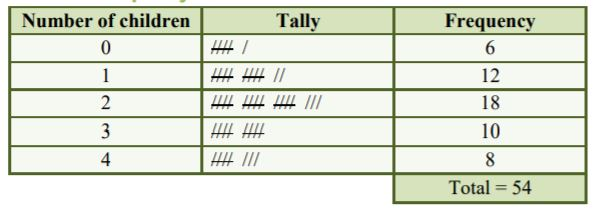
\includegraphics[width=0.7\linewidth]{images/image4} 

}

\caption{Frequency distribution table}\label{fig:freq}
\end{figure}

Now certain features of the data become apparent. For instance, it can easily be seen that, most of the 54 families selected have two children because number of houses having 2 children is 18. This information cannot easily be obtained from the raw data. The above table is called a frequency table or a frequency distribution. It is so called because it gives the frequency or number of times each
observation occurs. Thus, by finding the frequency of each observation, a more intelligible picture is obtained.

\hypertarget{construction-of-frequency-distribution}{%
\subsection{Construction of frequency distribution}\label{construction-of-frequency-distribution}}

\begin{enumerate}
\def\labelenumi{\arabic{enumi}.}
\item
  List all values of the variable in ascending order of magnitude.
\item
  Form a tally column, that is, for each value in the data, record a stroke in the tally column next to that value. In the tally, each fifth stroke is made across the first four. This makes it easy to count the entries and enter the frequency of each observation.
\item
  Check that the frequencies sum to the total number of observations
\end{enumerate}

\hypertarget{grouped-frequency-distribution}{%
\section{Grouped frequency distribution}\label{grouped-frequency-distribution}}

Data below gives the body masses of 22 patients, measured to the nearest kilogram.

\begin{figure}

{\centering 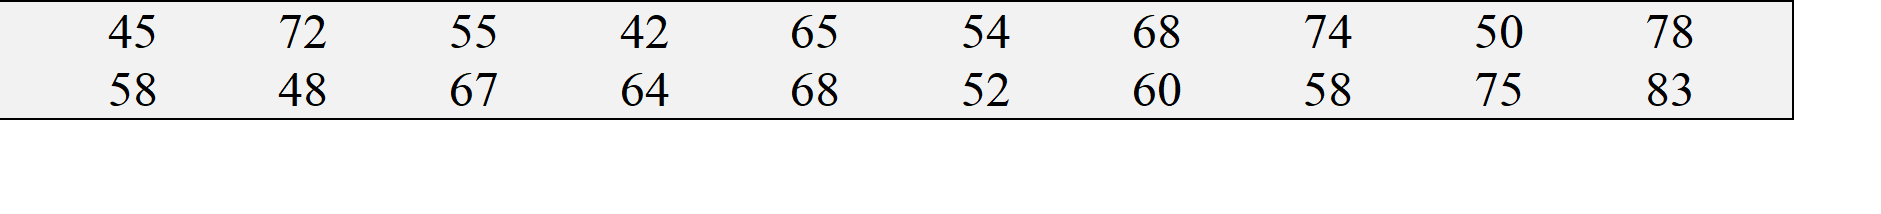
\includegraphics[width=0.7\linewidth]{images/image5} 

}

\caption{Body masses of 22 patients}\label{fig:mass}
\end{figure}

It can be seen that the minimum and the maximum body masses are 42 kg and 83 kg, respectively. A frequency distribution giving every body mass between 42 kg and 83 kg would be very long and would not be very informative. The problem is to overcome by grouping the data into classes.\\
If we choose the classes\\
41 -- 49\\
50 -- 58\\
59 -- 67\\
68 -- 76
and 77 -- 85, we obtain the frequency distribution given below:

\begin{figure}

{\centering 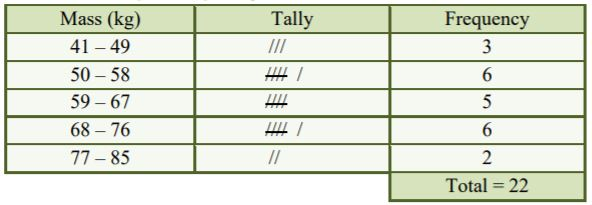
\includegraphics[width=0.7\linewidth]{images/image6} 

}

\caption{Grouped Frequency distribution table}\label{fig:grptable}
\end{figure}

Above table gives the frequency of each group or class; it is therefore called a grouped frequency table or a grouped frequency distribution. Using this grouped frequency distribution, it is easier to obtain information about the data than using the raw data. For instance, it can be seen that 17 of the 22 patients have body masses between 50 kg and 76 kg (both inclusive). This information cannot easily be obtained from the raw data.\\
It should be noted that, even though above table is concise, some information is lost. For example, the grouped frequency distribution does not give us the exact body masses of the patients. Thus the individual body masses of the patients are lost in our effort to obtain an overall picture.

\hypertarget{terms-used-in-grouped-frequency-tables.}{%
\section{Terms used in grouped frequency tables.}\label{terms-used-in-grouped-frequency-tables.}}

\textbf{Class limits}

The intervals into which the observations are put are called \underline{class intervals}. The end points of the class intervals are called \underline{class limits}. For example, the class interval 41 -- 49, has lower class limit 41 and upper class limit 49.

\textbf{Class boundaries}

The raw data in the above example were recorded to the nearest kilogram. Thus, a body mass of 49.5kg would have been recorded as 50 kg, a body mass of 58.4 kg would have been recorded as 58 kg, while a body mass of 58.5 kg would have been recorded as 59 kg. It can therefore be seen
that, the class interval 50 -- 58, consists of measurements greater than or equal to 49.5 kg and less than 58.5 kg. The numbers 49.5 and 58.5 are called the lower and upper boundaries of the class interval 50 -- 58. The class boundaries of the other class intervals are given below:

\begin{figure}

{\centering 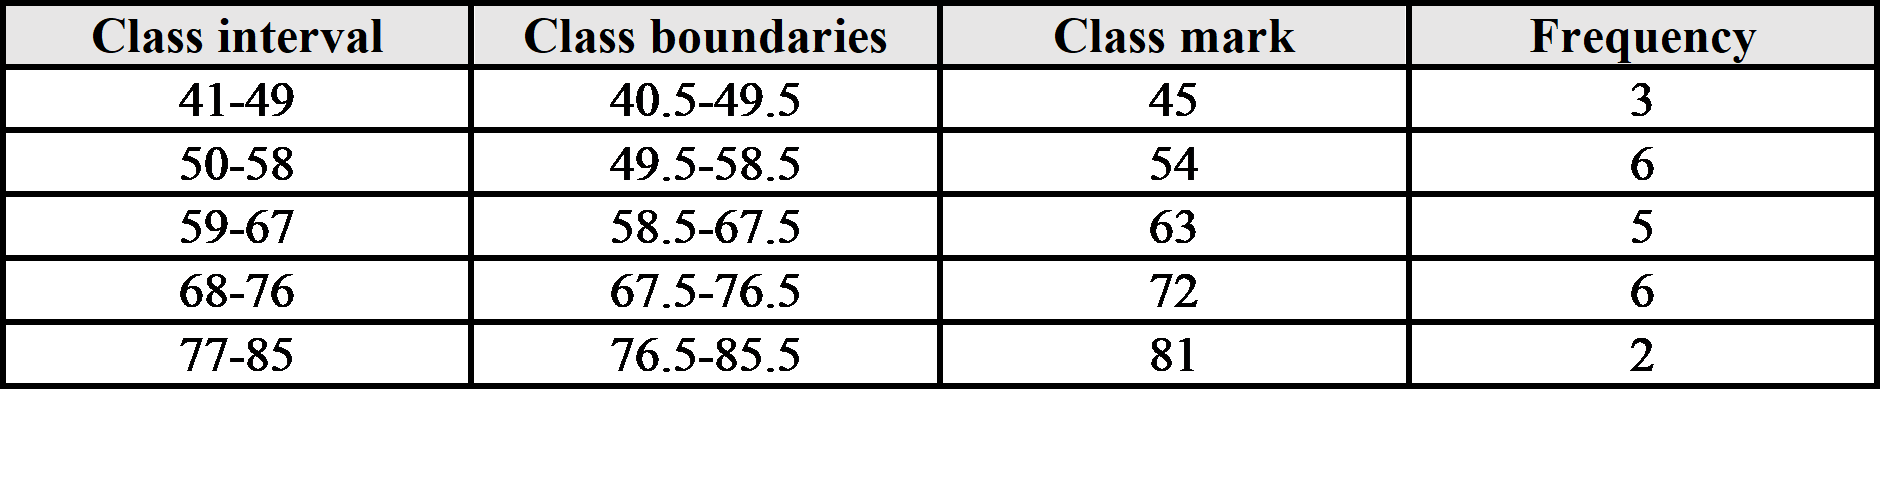
\includegraphics[width=0.7\linewidth]{images/image7} 

}

\caption{Class boundary and class limits}\label{fig:clsslmt}
\end{figure}

\underline{Note:}\\
Notice that the lower class boundary of the i\textsuperscript{th} class interval is the mean of the lower class limit of the class interval and the upper class limit of the (i-1)\textsuperscript{th} class interval (i = 2, 3, 4, \ldots). For example, in the table above the lower class boundaries of the second and the fourth class intervals are (50 + 49) /2 = 49.5 and (68 + 67)/2 = 67.5 respectively.\\
It can also be seen that the upper class boundary of the i\textsuperscript{th} class interval is the mean of the upper class limit of the class interval and the lower class limit of the (i+1)\textsuperscript{th} class interval (i = 1, 2, 3, \ldots). Thus, in the above table the upper class boundary of the fourth class
interval is (76 + 77)/2 = 76.5.

\textbf{Class mark}\\
The mid-point of a class interval is called the class mark or class mid-point of the class interval. It is the average of the upper and lower class limits of the class interval. It is also the average of the upper and lower class boundaries of the class interval. For example, in the table, the class mark of the third class interval was found as
follows: class mark =(59+67) /2 = (58.5 + 67.5)/2= 63.

\textbf{Class width}\\
The difference between the upper and lower class boundaries of a class interval is called the class width of the class interval. Class widths of class intervals can also be found by subtracting two consecutive lower class limits, or by subtracting two consecutive upper class limits.

\underline{Note:}

The width of the i\textsuperscript{th} class interval is the numerical difference between the upper class limits of the i\textsuperscript{th} and the ( i-1)\textsuperscript{th} class intervals (i = 2, 3, \ldots). It is also the numerical difference between the lower class limits of the i\textsuperscript{th} and the (i+1) \textsuperscript{th} class intervals (i = 1, 2, \ldots).

In grouped frequency table above the width of the first class interval is \textbar41-50\textbar{} = 9. This is the numerical difference between the lower class limits of the first and the second class intervals. The width of the second class interval is \textbar50-59\textbar= 9. This is the numerical difference between the lower class limits of the second and the third
class intervals. It is also equal to \textbar58-49\textbar{} the numerical, difference between the upper class limits of the first and the second class intervals.

\hypertarget{construction-of-frequency-distribution-table}{%
\section{Construction of frequency distribution table}\label{construction-of-frequency-distribution-table}}

\textbf{Step 1}. Decide how many classes you wish to use.\\
\textbf{Step 2}. Determine the class width\\
\textbf{Step 3}. Set up the individual class limits
\textbf{Step 4}. Tally the items into the classes\\
\textbf{Step 5}. Count the number of items in each class

Consider the example\\
An agricultural student measured the lengths of leaves on an oak tree (to the nearest cm). Measurements on 38 leaves are as follows\\
9,16,13,7,8,4,18,10,17,18,9,12,5,9,9,16,1,8,17,1,10,5,9,11,15,6,14,9,1,12,5,16,4,16,8,15,14,17

\textbf{Step 1.} Decide how many classes you wish to use.

H.A. Sturges provides a formula for determining the approximation number of classes. \(\mathbf{k = 1 + 3.322}\mathbf{\log}\mathbf{N}\)\textbf{.} Number of classes should be greater than calculated \emph{k}\\
In our example \emph{N}=38, so \emph{k}=1+3.322×log(38) = 1+3.322×1.5797 = 6.24 = approx 7

So the approximated number of classes should be not less than 6.24 \emph{i}.\emph{e}.\(\ k^{'}\) =7

\textbf{Step 2.} Determine the class width

Generally, the class width should be the same size for all classes. \emph{C}= \textbar{} max − min\textbar/ k. Class width \(C^{'}\)should be greater than calculated \emph{C}. For this example, \emph{C} = \textbar{} 18− 1\textbar/\textbf{6.24} = 2.72, so approximately class width\(C^{'} =\) 3 (Note that \emph{k} used here is the calculated value using Struges formula not the approximated).

\textbf{Step 3.} To set up the individual class limits, We need to find the lower limit only

\[L = min - \frac{C^{'} \times k^{'} - (max - min)}{2}\]

where C and \emph{k} here are final approximated class width and number of classes respectively in our example \(L = 1 - \frac{3 \times 7 - (18 - 1)}{2}\)=1-2=-1; since there is no negative values in data = 0.

\begin{table}[H]
\centering
\begin{tabular}[t]{cc}
\toprule
Class & Frequency\\
\midrule
0-3 & 3\\
3-6 & 5\\
6-9 & 5\\
9-12 & 9\\
12-15 & 5\\
\addlinespace
15-18 & 9\\
18-21 & 2\\
\bottomrule
\end{tabular}
\end{table}

Even though the student only measured in whole numbers, the data is continuous, so "4 cm" means the actual value could have been anywhere from 3.5 cm to 4.5 cm.

\hypertarget{cumulative-frequency}{%
\section{Cumulative frequency}\label{cumulative-frequency}}

In many situations, we are not interested in the number of observations in a given class interval, but in the number of observations which are less than (or greater than) a specified value. For example, in the above table, it can be seen that 3 leaves have length less than 3.5 cm and 9
leaves (i.e.~3 + 6) have length less than 6.5 cm. These frequencies are called cumulative frequencies. A table of such cumulative frequencies is called \textbf{a cumulative frequency table} or \textbf{cumulative frequency distribution}.

Cumulative frequency is defined as a running total of frequencies. Cumulative frequency can also defined as the sum of all previous frequencies up to the current point. Notice that the last cumulative frequency is equal to the sum of all the frequencies. Two types of cumulative frequencies are Less than cumulative frequency and Greater than cumulative frequency. Less than cumulative frequency
(LCF) is the number of values less than a specified value. Greater than cumulative frequency (GCF) is the number of observations greater than a specified value.

The specified value for LCF in the case of grouped frequency
distribution will be upper limits and for GCF will be the lower limits of the classes. LCF's are obtained by adding frequencies in the successive classes and GCF are obtained by subtracting the successive class frequencies from the total frequency.

\hypertarget{relative-frequency}{%
\section{Relative frequency}\label{relative-frequency}}

It is sometimes useful to know the proportion, rather than the number, of values falling within a particular class interval. We obtain this information by dividing the frequency of the particular class interval by the total number of observations. \textbf{Relative frequency} of a class
is the frequency of class / total observation. Relative frequencies all add up to 1.

\begin{table}[H]
\centering
\begin{tabular}[t]{ccccc}
\toprule
Class & Frequency & A & B & C\\
\midrule
0.5 – 3.5 & 3 & 3 & 38 & 0.078947\\
3.5 – 6.5 & 6 & 9 & 35 & 0.157895\\
6.5 – 9.5 & 10 & 19 & 29 & 0.263158\\
9.5 – 12.5 & 5 & 24 & 19 & 0.131579\\
12.5 – 15.5 & 5 & 29 & 14 & 0.131579\\
\addlinespace
15.5 – 18.5 & 9 & 38 & 9 & 0.236842\\
\bottomrule
\end{tabular}
\end{table}

{[}1{]} ``Note: A= Less than cumulative frequency; B= Greater than cumulative frequency, C = Relative frequency''

~\\
\hspace*{0.333em}\\
\hspace*{0.333em}

\hypertarget{hello}{}
\textbf{Data is the sword of the 21st century, those who wield it well, the Samurai.'' - Jonathan Rosenberg, former Google SVP}!

\hypertarget{graphical-representation-of-data}{%
\chapter{Graphical representation of data}\label{graphical-representation-of-data}}

We found that information given in a frequency distribution is easier to interpret than raw data. Information given in a frequency distribution in a tabular form is easier to grasp if presented graphically. Many types of diagrams are used in statistics, depending on the nature of the data and the purpose for which the diagram is intended.

\hypertarget{histogram}{%
\section{Histogram}\label{histogram}}

A histogram consists of rectangles with:

\begin{itemize}
\item
  Bases on a horizontal axis, centres at the class marks, and lengths equal to the class widths.
\item
  Areas proportional to class frequencies.
\end{itemize}

\underline{Note:}\\
If the class intervals are of equal size, then the heights of the rectangles are proportional to the class frequencies and it is then customary to take the heights of the rectangles numerically equal to the class frequencies. If the class intervals are of different widths, then
the heights of the rectangles are proportional to \(\frac{\text{Class Frequency}}{\text{Class Width}}\). This ratio is called \textbf{frequency density}.

Table below shows the frequency distribution of the body masses of 50 AIDS patients. Draw a Histogram.

\begin{longtable}[]{@{}lllllll@{}}
\toprule
Mass & 30 -- 39 & 40 -- 49 & 50 -- 59 & 60 -- 69 & 70 -- 79 & 80 -- 89 \\
\midrule
\endhead
Frequency & 3 & 6 & 17 & 13 & 8 & 3 \\
\bottomrule
\end{longtable}

\begin{figure}

{\centering 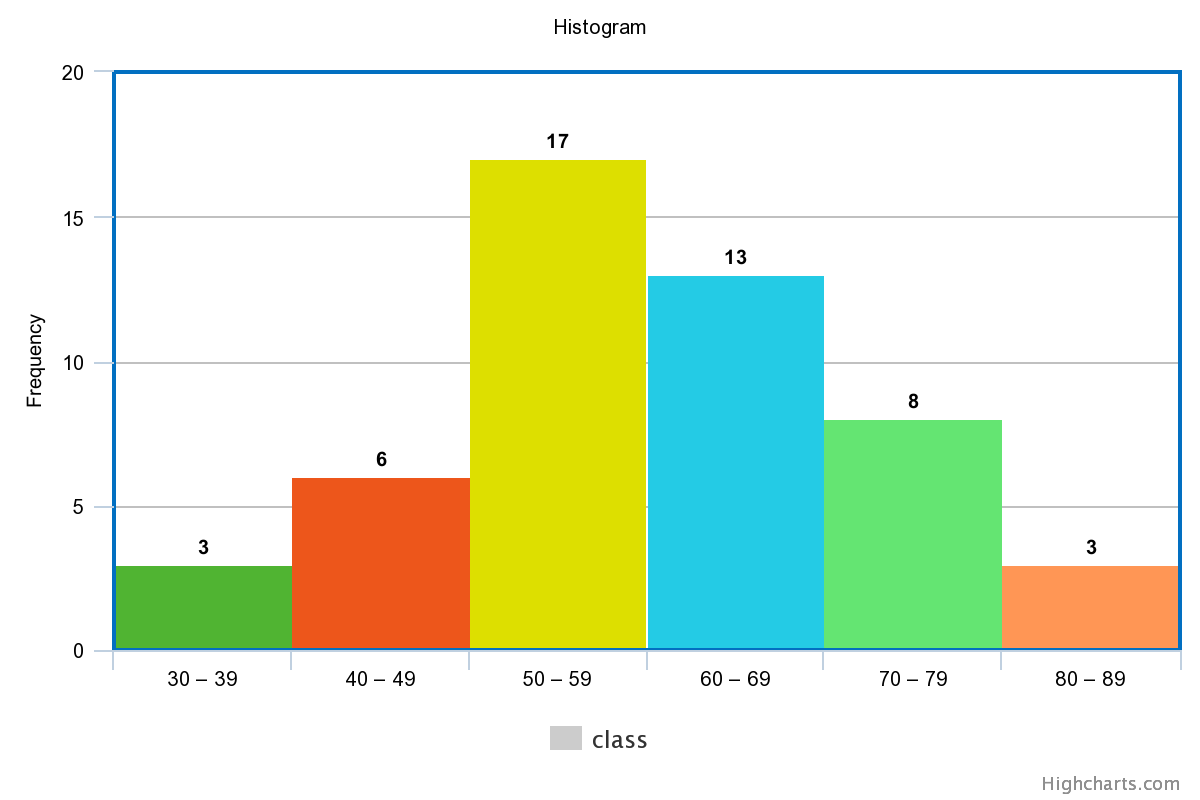
\includegraphics[width=0.7\linewidth]{images/image8} 

}

\caption{Histogram}\label{fig:hist1}
\end{figure}

\hypertarget{cumulative-frequency-curve-ogive}{%
\section{Cumulative frequency curve (Ogive)}\label{cumulative-frequency-curve-ogive}}

A graph obtained by plotting a cumulative frequency against the class boundary and joining the points by a smooth curve, is called a cumulative frequency curve. It is also called as Ogive. Two types of ogive are there, Less Than Type Cumulative Frequency Curve (Less than Ogive) and Greater Than Type Cumulative Frequency Curve (Greater than Ogive).

\hypertarget{less-than-ogive}{%
\subsection{Less than Ogive}\label{less-than-ogive}}

Also known as less than type cumulative frequency curve. Here we use the upper limit of the classes and the less than cumulative frequency to plot the curve. Let us see for the example of the body masses of 50 AIDS patients.

\begin{longtable}[]{@{}lllllll@{}}
\toprule
Upper limit & 39 & 49 & 59 & 69 & 79 & 89 \\
\midrule
\endhead
Less than Cumulative frequency & 3 & 9 & 26 & 39 & 47 & 50 \\
\bottomrule
\end{longtable}

\begin{figure}

{\centering 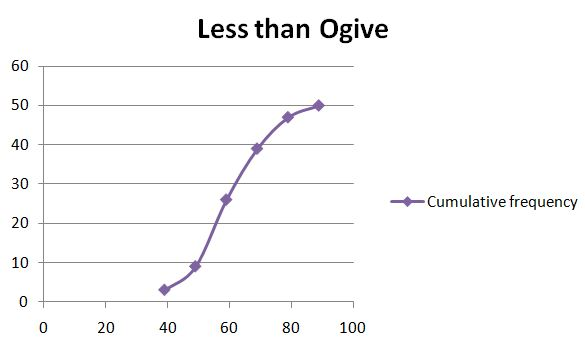
\includegraphics[width=0.7\linewidth]{images/image9} 

}

\caption{Less than ogive}\label{fig:lto}
\end{figure}

\hypertarget{greater-than-ogive}{%
\subsection{Greater than Ogive}\label{greater-than-ogive}}

Also known as greater than type cumulative frequency curve Here we use the lower limit of the classes and the greater than cumulative frequency to plot the curve.

\begin{longtable}[]{@{}lllllll@{}}
\toprule
Lower Limit & 30 & 40 & 50 & 60 & 70 & 80 \\
\midrule
\endhead
Greater than Cumulative frequency & 50 & 47 & 41 & 24 & 11 & 3 \\
\bottomrule
\end{longtable}

\begin{figure}

{\centering 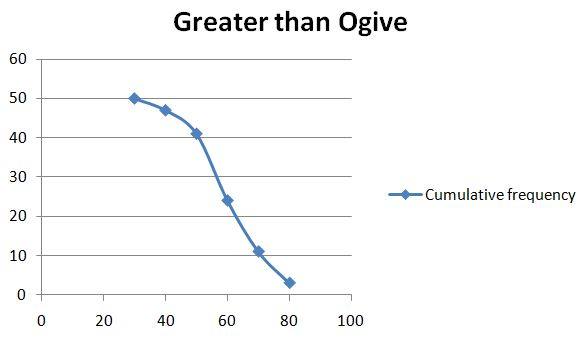
\includegraphics[width=0.7\linewidth]{images/image10} 

}

\caption{greater than ogive}\label{fig:gco}
\end{figure}

\underline{Note:}\\
Intersection of both ogives gives the median

\hypertarget{frequency-polygon}{%
\subsection{Frequency polygon}\label{frequency-polygon}}

A grouped frequency table can also be represented by a frequency
polygon, which is a special kind of line graph. To construct a frequency
polygon, we plot a graph of class frequencies against the corresponding
class mid-points and join successive points with straight lines. Frequency polygon is also obtained by joining the midpoints of a histogram as shown in Fig 2.5.

\begin{table}[H]
\centering
\begin{tabular}[t]{l|r|r|r|r|r|r}
\hline
Class Midpoints & 34.5 & 44.5 & 54.5 & 64.5 & 74.5 & 84.5\\
\hline
Frequencies & 3.0 & 6.0 & 17.0 & 13.0 & 8.0 & 3.0\\
\hline
\end{tabular}
\end{table}

\begin{figure}

{\centering 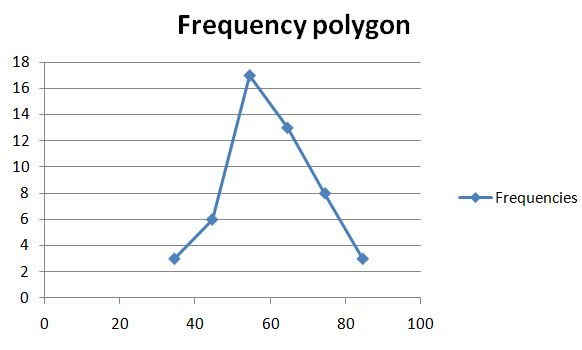
\includegraphics[width=0.7\linewidth]{images/image11} 

}

\caption{Frequency polygon}\label{fig:freqpol}
\end{figure}

\begin{figure}

{\centering 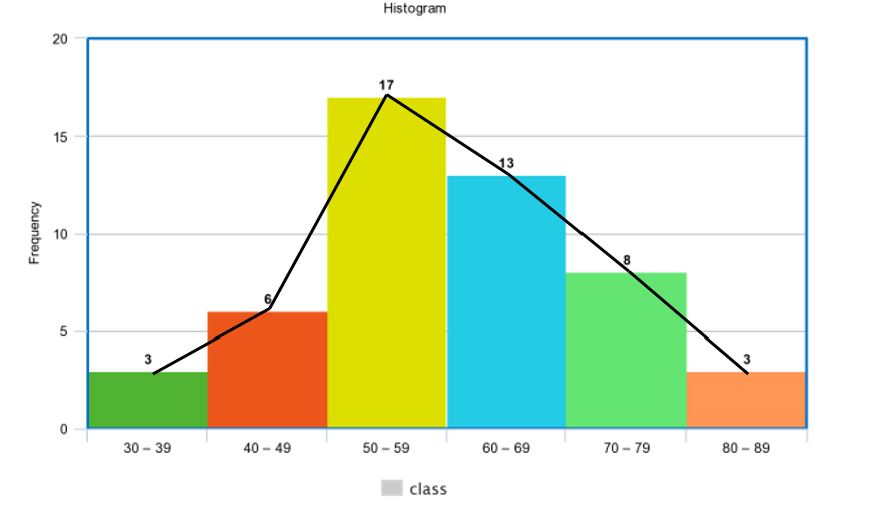
\includegraphics[width=0.7\linewidth]{images/image12} 

}

\caption{Frequency polygon and histogram}\label{fig:frehit}
\end{figure}

\hypertarget{stem-and-leaf-plot}{%
\section{Stem-and-leaf plot}\label{stem-and-leaf-plot}}

A stem-and-leaf plot is a graphical device that is useful for representing a relatively small set of data which takes numerical values. To construct a stem-and-leaf plot, we partition each measurement into two parts. The first part is called the stem, and the second part is called the leaf. Here each numerical value is divided into two parts:
The leading digits become the stem the trailing digits become the leaf. One advantage of the stem-and-leaf display over a frequency distribution is that we retain the value of each observation. Another is the distribution of the data within each groups is clear. A stem-and-leaf plot conveys similar information as a histogram. Turned on its side, it has the same shape as the histogram. In fact, since the
stem-and-leaf plot shows each observation,it displays information that is lost in a histogram. A properly
constructed stem-and-leaf plot, like a histogram, provides information regarding the range of the data set, shows the location of the highest concentration of measurements, and reveals the presence or absence of symmetry.

Consider the example

10,15,22,25,28,23,29,31,36,45,48

stem and leaf plot can be drawn as shown below.

\begin{table}[H]
\centering
\begin{tabular}[t]{cc}
\toprule
Stem & Leaf\\
\midrule
1 & 0 5\\
2 & 2 3 5 8 9\\
3 & 1 6\\
4 & 5 8\\
\bottomrule
\end{tabular}
\end{table}
\begin{figure}

{\centering 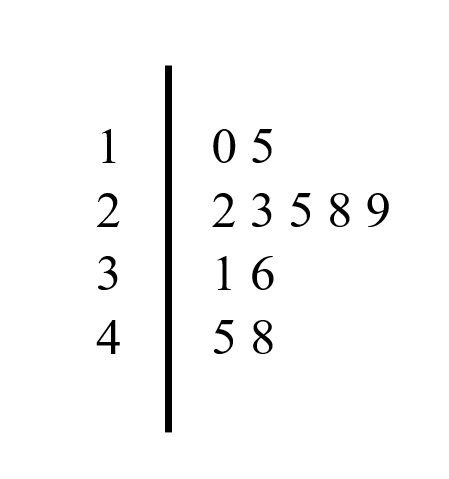
\includegraphics[width=0.3\linewidth]{images/image18} 

}

\caption{Stem and Leaf plot}\label{fig:stem}
\end{figure}

\hypertarget{bar-chart}{%
\section{Bar chart}\label{bar-chart}}

A bar chart or bar graph is a diagram consisting of a series of horizontal or vertical bars of equal width. The bars represent various categories of the data. There are three types of bar charts, and these are simple bar charts, component bar charts and grouped bar charts.

\hypertarget{simple-bar-chart}{%
\subsection{Simple bar chart}\label{simple-bar-chart}}

In a simple bar chart, the height (or length) of each bar is equal to the value of category in the y-axis it represents. For example data below shows the production of timber in five districts of Kerala in a certain year.

\begin{longtable}[]{@{}ll@{}}
\toprule
District & Production \\
\midrule
\endhead
Alappuzha & 600 \\
Kannur & 900 \\
Trissur & 1800 \\
Ernakulam & 1500 \\
Wayanad & 2400 \\
\bottomrule
\end{longtable}

\begin{figure}

{\centering 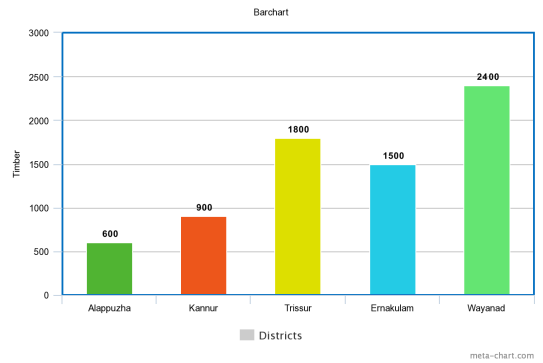
\includegraphics[width=0.5\linewidth]{images/image13} 

}

\caption{Barchart}\label{fig:bar}
\end{figure}

\hypertarget{component-bar-chart}{%
\subsection{Component bar chart}\label{component-bar-chart}}

In a component bar chart, the bar for each category is subdivided into component parts; hence its name. Component bar charts are therefore used to show the division of items into components. This is illustrated in the following example.

Example shows the distribution of sales of agricultural produce from a Farm in 1995, 1996 and 1997.

\begin{figure}

{\centering 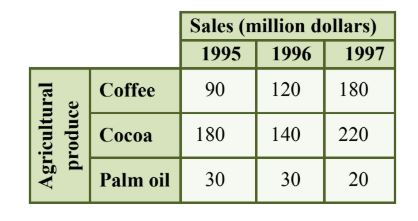
\includegraphics[width=0.5\linewidth]{images/image14} 

}

\caption{Sales data of agricultural produce}\label{fig:componentdata}
\end{figure}

\begin{figure}

{\centering 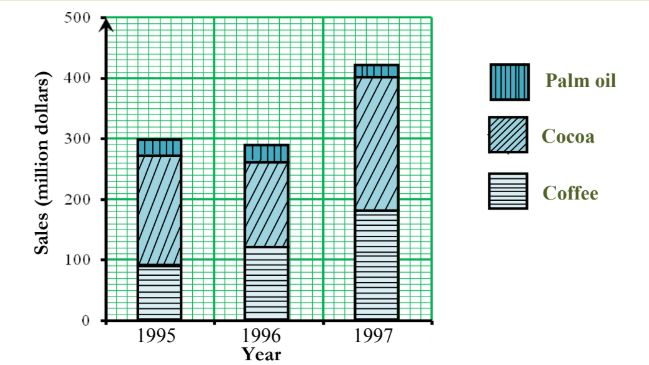
\includegraphics[width=0.5\linewidth]{images/image15} 

}

\caption{Component bar chart}\label{fig:componentbar}
\end{figure}

The component bar chart shows the changes of each component over the years as well as the comparison of the total sales between different years.

\hypertarget{grouped-bar-chart}{%
\subsection{Grouped bar chart}\label{grouped-bar-chart}}

For a grouped bar chart, the components are grouped together and drawn side by side. We illustrate this with the above example.

\begin{figure}

{\centering 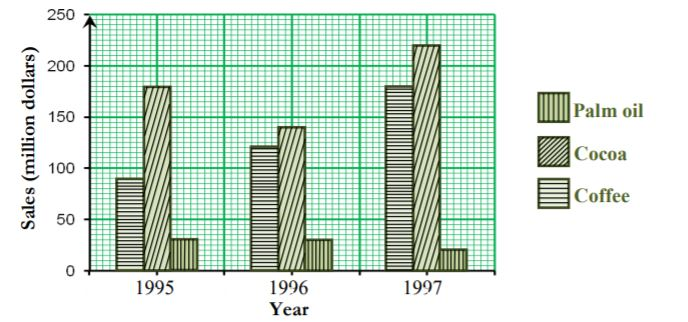
\includegraphics[width=0.7\linewidth]{images/image16} 

}

\caption{Grouped bar chart}\label{fig:groupbar}
\end{figure}

\hypertarget{histogram-and-bar-chart}{%
\section{Histogram and Bar chart}\label{histogram-and-bar-chart}}

\begin{longtable}[]{@{}
  >{\raggedright\arraybackslash}p{(\columnwidth - 4\tabcolsep) * \real{0.09}}
  >{\raggedright\arraybackslash}p{(\columnwidth - 4\tabcolsep) * \real{0.49}}
  >{\raggedright\arraybackslash}p{(\columnwidth - 4\tabcolsep) * \real{0.42}}@{}}
\toprule
Items & HISTOGRAM & BAR GRAPH \\
\midrule
\endhead
Meaning & Histogram refers to a graphical representation, that displays data by way of bars to show the frequency of numerical data. & Bar graph is a pictorial representation of data that uses bars to compare different categories of data. \\
Indicates & Distribution of non-discrete variables & Comparison of discrete variables \\
Presents & Quantitative data & Categorical data \\
Spaces & Bars touch each other, hence there are no spaces between bars & Bars do not touch each other, hence there are spaces between bars. \\
Elements & Elements are grouped together, so that they are considered as ranges. & Elements are taken as individual entities. \\
Can bars be reordered? & No & Yes \\
Width of bars & Need not to be same & Same \\
\bottomrule
\end{longtable}

\hypertarget{pie-charts}{%
\section{Pie Charts}\label{pie-charts}}

A pie chart is a circular graph divided into sectors, each sector representing a different value or category. The angle of each sector of a pie chart is proportional to the value of the part of the data it represents. The bar chart is more precise than the pie chart for visual comparison of categories with similar relative frequencies.

\hypertarget{steps-for-constructing-a-pie-chart}{%
\subsection{Steps for constructing a pie chart}\label{steps-for-constructing-a-pie-chart}}

\begin{enumerate}
\def\labelenumi{\arabic{enumi}.}
\tightlist
\item
  Find the sum of the category values.\\
\item
  Calculate the angle of the sector for each category, using the following formula.Angle of the sector for category A = \(\frac{\text{value of category A}}{\text{sum of category values}} \times 360\)\\
\item
  Construct a circle and mark the centre.\\
\item
  Use a protractor to divide the circle into sectors, using the angles obtained in step 2.\\
\item
  Label each sector clearly.
\end{enumerate}

See the example:\\
A lady spent the following sums of money on buying ingredients for a family Christmas cake.

\begin{longtable}[]{@{}lll@{}}
\toprule
Ingredients & Price & Angle \\
\midrule
\endhead
Flour & 24 & (24/240)×360= 36 \\
Margarine & 96 & 144 \\
Sugar & 18 & 27 \\
Eggs & 60 & 90 \\
Baking powder & 12 & 18 \\
Miscellaneous & 30 & 45 \\
\textbf{Total} & \textbf{240} & \textbf{360} \\
\bottomrule
\end{longtable}

\begin{figure}

{\centering 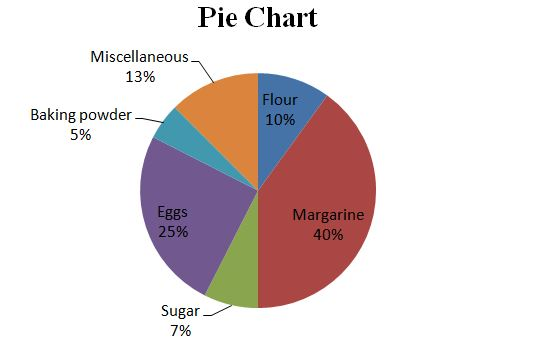
\includegraphics[width=0.5\linewidth]{images/image17} 

}

\caption{Pie chart}\label{fig:oiechart}
\end{figure}

~\\
\hspace*{0.333em}\\
\hspace*{0.333em}

\hypertarget{hello}{}
\textbf{Statistics is the grammar of science." - Karl Pearson}!

\hypertarget{measures-of-central-tendency---i}{%
\chapter{Measures of central tendency - I}\label{measures-of-central-tendency---i}}

In the previous lecture, you have learnt how data can be summarised in
the form of tables and presented in the form of graphs so that important
features can be illustrated easily and more effectively. In this
Lecture, we consider statistical measures which can be used to describe
the characteristics of a set of data.

We are interested in a single value that serves as a representative
value of the overall data. A~\textbf{measure of central tendency}~is a
summary statistic that represents the centre point or typical value of a
dataset.

There are five averages. Among them mean, median and mode are called
\textbf{simple averages} and the other two averages geometric mean and harmonic
mean are called \textbf{special averages}. These measures reflect numerical
values in the centre of a set of data and are therefore called measures
of central tendency.

{\textbf{Requisites of a Good Measure of Central Tendency:}}

\begin{itemize}
\item
  It should be rigidly defined.
\item
  It should be simple to understand \& easy to calculate
\item
  It should be based upon all values of given data
\item
  It should be capable of further mathematical treatment.
\item
  It should have sampling stability.
\item
  It should be not be unduly affected by extreme values
\end{itemize}

{The main objectives of Measure of Central Tendency}

\begin{itemize}
\item
  To condense data in a single value.
\item
  To facilitate comparisons between data.
\end{itemize}

\hypertarget{arithmetic-mean}{%
\section{Arithmetic Mean}\label{arithmetic-mean}}

This is what people usually intend when they say "average". Arithmetic
mean or simply the mean of a variable is defined as the sum of the
observations divided by the number of observations. Mean of set of
numbers \(x_{1\ },x_{2},\ldots,x_{n}\) is denoted as \(\overline{x}\). It is
given by the formula

\[\overline{x} = \frac{x_{1} + x_{2} + \ldots + x_{n}}{n}\]

\(= \frac{1}{n}\sum_{i = 1}^{n}x_{i}\)

\textbf{Example 3.1} Find the mean of the numbers 2, 4, 7, 8, 11, 12

\[\overline{x} = \frac{2 + 4 + 7 + 8 + 11 + 12}{6} = \frac{44}{6} = 7.33\]

\hypertarget{the-mean-of-a-frequency-distribution}{%
\subsection{The mean of a frequency distribution}\label{the-mean-of-a-frequency-distribution}}

\hypertarget{direct-method}{%
\subsubsection{Direct method}\label{direct-method}}

If the numbers \(x_{1\ },x_{2},\ldots,x_{n}\) occur with frequencies
\(f_{1\ },f_{2},\ldots,f_{n}\) respectively then

\[\overline{x} = \frac{x_{1}f_{1} + x_{2}f_{2\ \ } + \ldots + x_{n}f_{n}}{f_{1} + f_{2} + \ldots f_{n}}\]

\[= \frac{\sum_{i = 1}^{n}{f_{i}x_{i}}}{\sum_{i = 1}^{n}f_{i}}\]

\textbf{Example 3.2} Table below shows the body masses of 50 men. Find the
mean body mass.

\begin{longtable}[]{@{}llllll@{}}
\caption{\label{tab:bodymass} Body masses of 50 men.}\tabularnewline
\toprule
Mass(kg) & 59 & 60 & 61 & 62 & 63 \\
\midrule
\endfirsthead
\toprule
Mass(kg) & 59 & 60 & 61 & 62 & 63 \\
\midrule
\endhead
Frequency & 3 & 9 & 23 & 11 & 4 \\
\bottomrule
\end{longtable}

\textbf{Solution 3.2}

The calculation can be arranged as shown

\begin{longtable}[]{@{}lll@{}}
\toprule
Mass(\emph{x}) & Frequency(\emph{f}) & \emph{fx} \\
\midrule
\endhead
59 & 3 & 177 \\
60 & 9 & 540 \\
61 & 23 & 1403 \\
62 & 11 & 682 \\
63 & 4 & 252 \\
& \(\sum_{i = 1}^{n}f_{i}\)= 50 & \(\sum_{i = 1}^{n}{f_{i}x_{i}}\)= 3054 \\
\bottomrule
\end{longtable}

\(\overline{x} = \frac{\sum_{i = 1}^{n}{f_{i}x_{i}}}{\sum_{i = 1}^{n}f_{i}} = \frac{3054}{50}\)=
61.08 kg

\hypertarget{assumed-mean-method-indirect-method}{%
\subsubsection{Assumed mean method (Indirect method)}\label{assumed-mean-method-indirect-method}}

The amount of computation involved above can be reduced by using the
following formula:

\[\overline{x} = A + \frac{\sum_{i = 1}^{n}{f_{i}d_{i}}}{\sum_{i = 1}^{n}f_{i}}\]

Where \(A\) is the assumed mean, which can be any value in \emph{x}.
\(d_{i} = x_{i} - A\), \(f_{i}\) is the frequency of \(x_{i}\)

Consider the Example 2.2 see Table: \ref{tab:bodymass}

let \(A\) = 61; it can be any number in \emph{x}

\begin{longtable}[]{@{}rcrr@{}}
\toprule
Mass(\emph{x}) & Frequency(\emph{f}) & \(\mathbf{d}_{\mathbf{i}}\mathbf{=}\mathbf{x}_{\mathbf{i}}\mathbf{-}\mathbf{61}\) & \(\mathbf{f}_{\mathbf{i}}\mathbf{d}_{\mathbf{i}}\) \\
\midrule
\endhead
59 & 3 & -2 & -6 \\
60 & 9 & -1 & -9 \\
61 & 23 & 0 & 0 \\
62 & 11 & 1 & 11 \\
63 & 4 & 2 & 8 \\
& \(\sum_{i = 1}^{n}f_{i}\)= 50 & & \(\sum_{i = 1}^{n}{f_{i}d_{i}}\)= 4 \\
\bottomrule
\end{longtable}

\(\overline{x} = 61 + \frac{4}{50}\) = 61.08 kg

The mean mass is 61.08 kg

\hypertarget{mean-of-grouped-data}{%
\subsection{Mean of Grouped Data}\label{mean-of-grouped-data}}

\hypertarget{direct-method-1}{%
\subsubsection{Direct method}\label{direct-method-1}}

The mean for grouped data is obtained from the following formula:

\[\overline{x} = \frac{\sum_{i = 1}^{k}{f_{i}x_{i}}}{n}\]

Where \(x_{i}\) = the mid-point of \emph{i}\textsuperscript{th} class (\emph{i}\textsuperscript{th} class mark);
\(f_{i}\)= the frequency of \emph{i}\textsuperscript{th} class; \(n\) = the sum of the
frequencies or total frequencies in a sample. Note that \emph{i} =1,2...,
\emph{k}, \emph{i}.\emph{e}. there are \emph{k} classes.

\textbf{Example 3.3} Shows the distribution of the marks scored by 60 students in a Physics examination. Find the mean mark.

\begin{longtable}[]{@{}llllll@{}}
\caption{\label{tab:phy} Distribution of the marks scored by 60 students}\tabularnewline
\toprule
Mark (\%) & 60-65 & 65-70 & 70-75 & 75-80 & 80-85 \\
\midrule
\endfirsthead
\toprule
Mark (\%) & 60-65 & 65-70 & 70-75 & 75-80 & 80-85 \\
\midrule
\endhead
Number of students & 2 & 15 & 25 & 14 & 4 \\
\bottomrule
\end{longtable}

\textbf{Solution 3.3}

The solution can be arranged as shown

\begin{longtable}[]{@{}llll@{}}
\toprule
Marks & Class mark(\(\mathbf{x}_{\mathbf{i}}\)) & Frequency(\(\mathbf{f}_{\mathbf{i}}\)) & \(\mathbf{f}_{\mathbf{i}}\mathbf{x}_{\mathbf{i}}\) \\
\midrule
\endhead
60-65 & 62.5 & 2 & 125 \\
65-70 & 67.5 & 15 & 1012.5 \\
70-75 & 72.5 & 25 & 1812.5 \\
75-80 & 77.5 & 14 & 1085 \\
80-85 & 82.5 & 4 & 330 \\
& & \(\sum_{i = 1}^{n}f_{i}\)= 60 & \(\sum_{i = 1}^{n}{f_{i}x_{i}}\)= 4365 \\
\bottomrule
\end{longtable}

\(\overline{x} = \frac{\sum_{i = 1}^{n}{f_{i}x_{i}}}{\sum_{i = 1}^{n}f_{i}} = \frac{4365}{60}\)=
72.75

The mean mark is 72.75\%

\hypertarget{coding-method-indirect-method}{%
\subsubsection{Coding method (Indirect method)}\label{coding-method-indirect-method}}

If all the class intervals of a grouped frequency distribution have equal size \(C\) (class width); then the following formula can be used instead of direct method above. This formula makes calculations easier.

\[\overline{x} = A + C\frac{\sum_{i = 1}^{n}{f_{i}u_{i}}}{\sum_{i = 1}^{n}f_{i}}\]

Where \(A\) is the he class mark with the highest frequency,
\(u_{i} = \frac{x_{i} - A}{C}\), \(f_{i}\) is the frequency of \(x_{i}\), \emph{C}
is the class width

This is called the ``coding'' method for computing the mean. It is a very short method and should always be used for finding the mean of a grouped frequency distribution with equal class widths.

Consider the Example 3.3 see Table:\ref{tab:phy}

\(A\)=72.5, class mark with highest frequency; \(C\) =5

\begin{longtable}[]{@{}lllll@{}}
\toprule
Marks & Class mark(\(\mathbf{x}_{\mathbf{i}}\)) & Frequency(\(\mathbf{f}_{\mathbf{i}}\)) & \(\mathbf{u}_{\mathbf{i}}\mathbf{=}\frac{\mathbf{x}_{\mathbf{i}}\mathbf{- 72.5}}{\mathbf{5}}\) & \(\mathbf{f}_{\mathbf{i}}\mathbf{u}_{\mathbf{i}}\) \\
\midrule
\endhead
60-65 & 62.5 & 2 & -2 & -4 \\
65-70 & 67.5 & 15 & -1 & -15 \\
70-75 & 72.5 & 25 & 0 & 0 \\
75-80 & 77.5 & 14 & 1 & 14 \\
80-85 & 82.5 & 4 & 2 & 8 \\
& & \(\sum_{i = 1}^{k}f_{i}\)= 60 & & \(\sum_{i = 1}^{k}{f_{i}u_{i}}\)=3 \\
\bottomrule
\end{longtable}

\(\overline{x} = 72.5 + 5 \times \left( \frac{3}{60} \right)\)= 72.75

The mean mark is 72.75\%

\hypertarget{merits-and-demerits-of-arithmetic-mean-merits}{%
\section{Merits and demerits of Arithmetic mean Merits}\label{merits-and-demerits-of-arithmetic-mean-merits}}

\underline{\textbf{Merits }}

\begin{enumerate}
\def\labelenumi{\arabic{enumi}.}
\item
  It is rigidly defined.
\item
  It is easy to understand and easy to calculate.
\item
  If the number of items is sufficiently large, it is more accurate
  and more reliable.
\item
  It is a calculated value and is not based on its position in the
  series.
\item
  It is possible to calculate even if some of the details of the data
  are lacking.
\item
  Of all averages, it is affected least by fluctuations of sampling.
\item
  It provides a good basis for comparison.
\end{enumerate}

\underline{\textbf{Demerits}}

\begin{enumerate}
\def\labelenumi{\arabic{enumi}.}
\item
  It cannot be obtained by inspection nor located through a frequency
  graph.
\item
  It cannot be in the study of qualitative phenomena not capable of
  numerical measurement \emph{i}.\emph{e}. Intelligence, beauty, honesty etc.
\item
  It can ignore any single item only at the risk of losing its
  accuracy.
\item
  It is affected very much by extreme values.
\item
  It cannot be calculated for open-end classes.
\item
  It may lead to fallacious conclusions, if the details of the data
  from which it is computed are not given.
\end{enumerate}

\hypertarget{the-median}{%
\section{The median}\label{the-median}}

\textbf{The median} of a set of data is defined as the middle value when the
data is arranged in order of magnitude. If there are no ties, half of
the observations will be smaller than the median, and half of the
observations will be larger than the median. The median can be the
middle most item that divides the group into two equal parts, one part
comprising all values greater, and the other, all values less than that
item. It is a positional measure.

\hypertarget{median-of-ungrouped-or-raw-data}{%
\subsection{Median of ungrouped or raw data}\label{median-of-ungrouped-or-raw-data}}

Arrange the given \emph{n} observations \(x_{1\ },x_{2},\ldots,x_{n}\) in
ascending order. If the number of values is odd, median is the middle
value. If the number of values is even, median is the mean of middle two
values.

Arrange data in ascending then use the following formula

When \emph{n} is odd, Median = Md
=\(\left( \frac{n + 1}{2} \right)^{\text{th}}\)value

When \emph{n} is even, Median = Md
=\({\text{Average\ of\ }\left( \frac{n}{2} \right)^{th}\text{and\ }\left( \frac{n}{2} + 1 \right)}^{\text{th}}\)value

\textbf{Example 3.4} Find the median of each of the following sets of
numbers.

(a) 12, 15, 22, 17, 20, 26, 22, 26, 12

(b) 4, 7, 9, 10, 5, 1, 3, 4, 12, 10

\textbf{Solution 3.4}

(a) Arranging the data in an increasing order of magnitude, we
obtain 12, 12, 15, 17, 20, 22, 22, 26, 26. Here, N (= 9) is odd, and so,
median =\(\left( \frac{9 + 1}{2} \right)^{\text{th}}\)= 5\textsuperscript{th} ordered
observation = 20.

Note: If a number is repeated, we still count it the number of times it
appears when we calculate the median.

(b) Arranging the data in an increasing order of magnitude, we obtain
1, 3, 4, 4, 5, 7, 9, 10, 10, 12. Here, N(=10) is an even number and so
median = \(\frac{1}{2}\)\{5\textsuperscript{th} ordered observation + 6\textsuperscript{th} ordered
observation\} = \(\frac{1}{2}\left( 5 + 7 \right) = 6\).

Note: You can see in each case, the median divides the distribution into
two equal parts, with 50\% of the observations greater than it and the
other 50\% less than it.

\hypertarget{median-of-ungrouped-frequency-distribution}{%
\subsection{Median of ungrouped frequency distribution}\label{median-of-ungrouped-frequency-distribution}}

The median is the middle number is an ordered set of data. In a
frequency table, the observations are already arranged in an ascending
order. We can obtain the median by looking for the value in the middle
position.

\hypertarget{median-of-a-frequency-table-when-the-number-of-observations-is-odd}{%
\subsubsection{Median of a frequency table when the number of observations is odd}\label{median-of-a-frequency-table-when-the-number-of-observations-is-odd}}

When the number of observations (n) is odd, then the median is the value
at the~\(\left( \frac{n + 1}{2} \right)^{\text{th}}\) positional value.
For that we use less than cumulative frequency.

\textbf{Example 3.5}: The following is a frequency table of the score obtained in a mathematics quiz. Find the median score.

\begin{longtable}[]{@{}llllll@{}}
\caption{\label{tab:score} Score obtained in a mathematics quiz.}\tabularnewline
\toprule
\textbf{Score} & 0 & 1 & 2 & 3 & 4 \\
\midrule
\endfirsthead
\toprule
\textbf{Score} & 0 & 1 & 2 & 3 & 4 \\
\midrule
\endhead
\textbf{Frequency} & 3 & 4 & 7 & 6 & 3 \\
\bottomrule
\end{longtable}

\textbf{Solution 3.5:}

Total frequency = 3 + 4 + 7 + 6 + 3 = 23 (odd number). Since the number
of scores is odd, the median is at
\(\left( \frac{23 + 1}{2} \right)^{\text{th}} =\) 12\textsuperscript{th}~position. To find
out the 12\textsuperscript{th}~position, we use less than cumulative frequencies as
shown:

\begin{longtable}[]{@{}llllll@{}}
\toprule
\textbf{Score} & 0 & 1 & \textbf{2} & 3 & 4 \\
\midrule
\endhead
\textbf{Frequency} & 3 & 4 & \textbf{7} & 6 & 3 \\
\textbf{less than cumulative frequency} & 3 & 7 & \textbf{14} & 20 & 23 \\
\bottomrule
\end{longtable}

The 12\textsuperscript{th}~position is after the 7\textsuperscript{th}~position but before the
14\textsuperscript{th}~position. So, the median is 2.

\hypertarget{median-of-a-frequency-table-when-the-number-of-observations-is-even}{%
\subsubsection{Median of a frequency table when the number of observations is even}\label{median-of-a-frequency-table-when-the-number-of-observations-is-even}}

When the number of observations is even, then the median is the average
of
\({\left( \frac{n}{2} \right)^{th}\text{and\ }\left( \frac{n}{2} + 1 \right)}^{\text{th}}\)
position values.

\textbf{Example 3.6}: The table is a frequency table of the marks obtained in a competition. Find the median score.

\begin{longtable}[]{@{}llllll@{}}
\caption{\label{tab:median} Distribution of marks obtained in a competition.}\tabularnewline
\toprule
\textbf{Mark} & 0 & 1 & 2 & 3 & 4 \\
\midrule
\endfirsthead
\toprule
\textbf{Mark} & 0 & 1 & 2 & 3 & 4 \\
\midrule
\endhead
\textbf{Frequency} & 11 & 9 & 5 & 10 & 15 \\
\bottomrule
\end{longtable}

\textbf{Solution 3.6}:

Total frequency = 11 + 9 + 5 + 10 + 15 = 50 (even number). Since the
number of scores is even, the median is at the average of the~values in
\({\left( \frac{n}{2} \right)^{th} = 25\ and\ \left( \frac{n}{2} + 1 \right)}^{\text{th}} = 26\)
positions. To find out the 25\textsuperscript{th}~position and 26\textsuperscript{th}~position, we add up the frequencies as shown:

\begin{longtable}[]{@{}llllll@{}}
\toprule
\textbf{Mark} & 0 & 1 & 2 & 3 & 4 \\
\midrule
\endhead
\textbf{Frequency} & 11 & 9 & 5 & 10 & 15 \\
\textbf{less than cumulative frequency} & 11 & 20 & 25 & 35 & 50 \\
\bottomrule
\end{longtable}

The mark at the 25\textsuperscript{th}~position is 2 and the mark at the 26\textsuperscript{th}~position
is 3. The median is the average of the scores at 25\textsuperscript{th}~and
26\textsuperscript{th}~positions =~\(\frac{2 + 3}{2} = 2.5\)

\hypertarget{median-of-grouped-frequency-distribution}{%
\subsection{Median of grouped frequency distribution}\label{median-of-grouped-frequency-distribution}}

The exact value of the median of a grouped data cannot be obtained
because the actual values of a grouped data are not known. For a grouped
frequency distribution, the median is in the class interval which
contains the \(\left( \frac{N}{2} \right)^{\text{th}}\)ordered
observation, where \(N\) is the total number of observations. This class
interval is called the \textbf{median class}. The median of a grouped
frequency distribution can be estimated by either of the following two
methods:

\hypertarget{linear-interpolation-method-for-estimating-the-median}{%
\subsubsection{Linear interpolation method for estimating the median}\label{linear-interpolation-method-for-estimating-the-median}}

The median of a grouped frequency distribution can be estimated by
linear interpolation. We assume that the observations are evenly spread
through the median class. The median can then be computed by using the
following formula:

\[median = L + \left( \frac{\frac{1}{2}N - F}{f_{m}} \right)C\]

where \(N\) = total number of observations, \(L\) = lower limit of the
median class, \(F\) = sum of all frequencies below \emph{L}(cumulative
frequency), \(f_{m}\) = frequency of the median class, \(C\) = class width
of the median class.

\hypertarget{estimation-of-the-median-from-a-cumulative-frequency-curve}{%
\subsubsection{Estimation of the median from a cumulative frequency curve}\label{estimation-of-the-median-from-a-cumulative-frequency-curve}}

The median of a grouped frequency distribution can be estimated from a
cumulative frequency curve. A horizontal line is drawn from the point
\(\frac{\text{N\ }}{2}\) on the vertical axis to meet the cumulative
frequency curve. From the point of intersection, a vertical line is
dropped to the horizontal axis. The value on the horizontal axis is
equal to the median.\\

\begin{figure}

{\centering 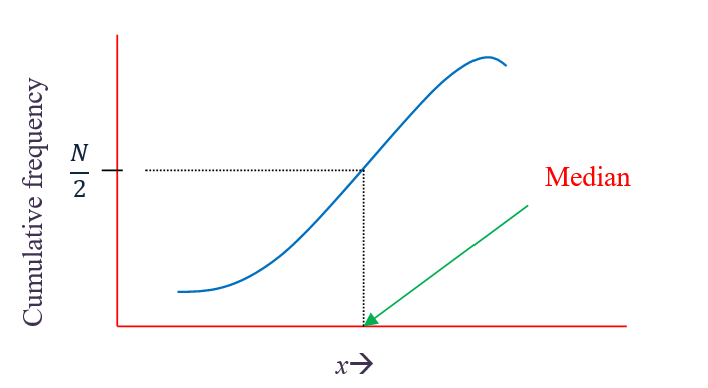
\includegraphics[width=0.4\linewidth]{images/mediancf} 

}

\caption{median from a cumulative frequency curve }\label{fig:mediancf}
\end{figure}

\textbf{Example 3.7} Table below gives the distribution of the heights of 60
students in a Senior High school. Find the median height of the students

\begin{longtable}[]{@{}lllllll@{}}
\caption{\label{tab:medianheight}Distribution of heights of 60
students}\tabularnewline
\toprule
Height(cm) & 145-150 & 150-155 & 155-160 & 160-165 & 165-170 & 170-175 \\
\midrule
\endfirsthead
\toprule
Height(cm) & 145-150 & 150-155 & 155-160 & 160-165 & 165-170 & 170-175 \\
\midrule
\endhead
Number of students & 3 & 9 & 16 & 18 & 10 & 4 \\
\bottomrule
\end{longtable}

\textbf{Solution 3.7}

\textbf{(i) Linear interpolation method for estimating the median}

\(N\) = 60

Median class= class interval which contains the
\(\left( \frac{N}{2} \right)^{\text{th}}\)ordered observation; here
\(\left( \frac{60}{2} \right)^{\text{th}} =\) 30\textsuperscript{th} observation. Before
the class 160-165 there are 3+9+16=28 observations so 30\textsuperscript{th} observation
will be in the class 160-165, therefore it is the median class.

\(L\) = lower limit of the median class =160

\(F\) = sum of all frequencies below 160(cumulative frequency) = 16+9+3=
28

\(f_{m}\) = frequency of the median class=18

\(C\) = class width of the median class=5

\(median = 160 + \left( \frac{\frac{1}{2}60 - 28}{18} \right)5\) = 160.56

\textbf{(ii) Estimation of the median from a cumulative frequency curve}

\begin{figure}

{\centering 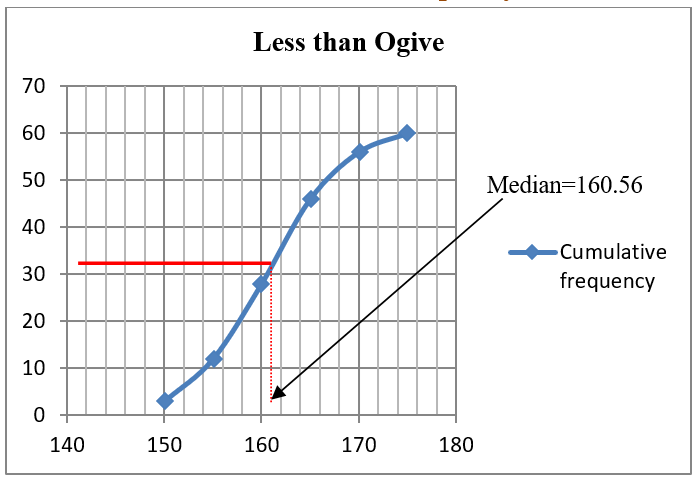
\includegraphics[width=0.4\linewidth]{images/cf} 

}

\caption{Median from a cumulative frequency curve Example 3.7}\label{fig:mediancf1}
\end{figure}

\hypertarget{merits-and-demerits-of-median}{%
\section{Merits and Demerits of Median}\label{merits-and-demerits-of-median}}

\underline{\textbf{Merits}}

\begin{enumerate}
\def\labelenumi{\arabic{enumi}.}
\item
  Median is not influenced by extreme values because it is a
  positional average.
\item
  Median can be calculated in case of distribution with open-end
  intervals
\item
  Median can be located even if the data are incomplete.
\end{enumerate}

\underline{\textbf{Demerits}}

\begin{enumerate}
\def\labelenumi{\arabic{enumi}.}
\item
  A slight change in the series may bring drastic change in median
  value.
\item
  In case of even number of items or continuous series, median is an
  estimated value other than any value in the series.
\item
  It is not suitable for further mathematical treatment except its use
  in calculating mean deviation.
\item
  It does not take into account all the observations
\end{enumerate}

\hypertarget{the-mode}{%
\section{The mode}\label{the-mode}}

The mode of a set of data is the value which occurs with the greatest
frequency. The mode is therefore the most common value. The mode is an
important measure in case of qualitative data. The mode can be used to
describe both quantitative and qualitative data.

\hypertarget{mode-of-ungrouped-or-raw-data}{%
\subsection{Mode of ungrouped or raw data}\label{mode-of-ungrouped-or-raw-data}}

For ungrouped data or a series of individual observations, mode is often
found by mere inspection.

\textbf{Example 3.8}

(a) The mode of 1, 2, 2, 2, 3 is 2.

(b) The modes of 2, 3, 4, 4, 5, 5 are 4 and 5.

(c) The mode does not exist when every observation has the same frequency. For example, the following sets of data have no modes: (i) 3,
6, 8, 9; (ii) 4, 4, 4, 7, 7, 7, 9, 9, 9.

Note: It can be seen that the mode of a distribution may not exist, and
even if it exists, it may not be unique. Distributions with a single
mode are referred to as \emph{unimodal}. Distributions with two modes are
referred to as \emph{bimodal}. Distributions may have several modes, in which
case they are referred to as \emph{multimodal}.

\textbf{Example 3.9} 20 patients selected at random had their blood groups
determined. The results are given in the table below

\begin{longtable}[]{@{}lllll@{}}
\caption{\label{tab:Blood} Blood groups of 20 patients}\tabularnewline
\toprule
Blood group & A & AB & B & O \\
\midrule
\endfirsthead
\toprule
Blood group & A & AB & B & O \\
\midrule
\endhead
No.~of patients & 2 & 4 & 6 & 8 \\
\bottomrule
\end{longtable}

The blood group with the highest frequency is O. The mode of the data is
therefore blood group O. We can say that most of the patients selected
have blood group O. Notice that the mean and the median cannot be
applied to the data. This is because the variable ``blood group'' cannot
take numerical values. However, it can be seen that the mode can be used
to describe both quantitative and qualitative data.

\hypertarget{mode-of-grouped-frequency-distribution}{%
\subsection{Mode of Grouped frequency distribution}\label{mode-of-grouped-frequency-distribution}}

\[mode = L + \left( \frac{f_{s}}{f_{p} + f_{s}} \right)C\]

Locate the highest frequency the class corresponding to that frequency
is called the \textbf{modal class}.

Where \(L\) = lower limit of the model class; \(f_{p}\)= the frequency of
the class preceding the model class; \(f_{s}\)= the frequency of the class
succeeding the model class and \(C\) = class interval

\textbf{Example 3.10} For the frequency distribution of weights of sorghum
ear-heads given in table below. Calculate the mode.

\begin{longtable}[]{@{}ll@{}}
\caption{\label{tab:earhead}requency distribution of weights of sorghum ear heads}\tabularnewline
\toprule
Weights of ear heads (g) & No of ear heads (\emph{f}) \\
\midrule
\endfirsthead
\toprule
Weights of ear heads (g) & No of ear heads (\emph{f}) \\
\midrule
\endhead
60-80 & 22 \\
80-100 & 38 \\
100-120 & 45 \\
120-140 & 35 \\
140-160 & 20 \\
\bottomrule
\end{longtable}

Modal class is \textbf{100-120}

\(mode = 100 + \left( \frac{35}{38 + 35} \right)20 =\) 109.589

\hypertarget{mode-using-histogram}{%
\subsection{\texorpdfstring{\textbf{Mode using Histogram}}{Mode using Histogram}}\label{mode-using-histogram}}

Consider the figure below. The modal class is the class interval which
corresponds to rectangle \(\text{ABCD}\). An estimate of the mode of the
distribution is the abscissa of the point of intersection of the line
segments \(\overline{\text{AE}}\)and \(\overline{\text{BF}}\)in

\begin{figure}

{\centering 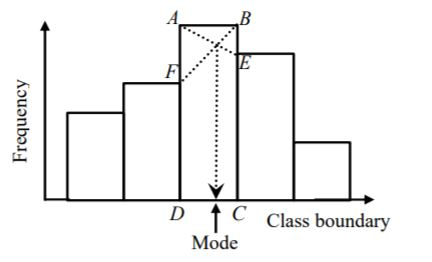
\includegraphics[width=0.4\linewidth]{images/l2m1} 

}

\caption{Median from a cumulative frequency curve for Example 3.10}\label{fig:cf1}
\end{figure}

\hypertarget{merits-and-demerits-of-mode}{%
\section{Merits and Demerits of Mode}\label{merits-and-demerits-of-mode}}

\underline{\emph{Merits}}

\begin{enumerate}
\def\labelenumi{\arabic{enumi}.}
\item
  It is readily comprehensible and easy to compute. In some case it
  can be computed merely by inspection.
\item
  It is not affected by extreme values. It can be obtained even if the
  extreme values are not known.
\item
  Mode can be determined in distributions with open classes.
\item
  Mode can be located on the graph also.
\item
  Mode can be used to describe both quantitative and qualitative data.
\end{enumerate}

\underline{\emph{Demerits}}

\begin{enumerate}
\def\labelenumi{\arabic{enumi}.}
\item
  The mode is not unique. That is, there can be more than one mode for
  a given set of data.
\item
  The mode of a set of data may not exist
\item
  It is not based upon all the observation.
\end{enumerate}

~\\
\hspace*{0.333em}\\
\hspace*{0.333em}

\hypertarget{hello}{}
\textbf{If the statistics are boring, you've got the wrong numbers}!

\hypertarget{measures-of-central-tendency--ii}{%
\chapter{Measures of central tendency -II}\label{measures-of-central-tendency--ii}}

\hypertarget{geometric-mean}{%
\section{Geometric mean}\label{geometric-mean}}

The geometric mean is a type of average, usually used for growth rates,
like population growth or interest rates. While the arithmetic mean adds
items, the geometric mean multiplies items.

The geometric mean of a series containing \emph{n} observations is the
\emph{n}\textsuperscript{th} root of the product of the values. If
\(x_{1},\ x_{2},\ldots,\ x_{n}\ \)are observations then

\[\mathbf{\text{Geometric mean}}\mathbf{,\ }\mathbf{GM =}\sqrt[\mathbf{n}]{\mathbf{x}_{\mathbf{1}}\mathbf{x}_{\mathbf{2}}\mathbf{\ldots}\mathbf{x}_{\mathbf{n}}}\]

\[\mathbf{=}\left( \mathbf{x}_{\mathbf{1}}\mathbf{x}_{\mathbf{2}}\mathbf{\ldots}\mathbf{x}_{\mathbf{n}} \right)^{\frac{\mathbf{1}}{\mathbf{n}}}\]

\[\mathbf{\log}\mathbf{\text{GM}}\mathbf{=}\frac{\mathbf{1}}{\mathbf{n}}\mathbf{\log}\left( \mathbf{x}_{\mathbf{1}}\mathbf{x}_{\mathbf{2}}\mathbf{\ldots}\mathbf{x}_{\mathbf{n}} \right)\]

\[\mathbf{=}\frac{\mathbf{1}}{\mathbf{n}}\left( \mathbf{\log}\mathbf{x}_{\mathbf{1}}\mathbf{+}\mathbf{\log}\mathbf{x}_{\mathbf{2}}\mathbf{\ldots +}\mathbf{\log}\mathbf{x}_{\mathbf{n}} \right)\]

\[\mathbf{=}\frac{\sum_{\mathbf{i = 1}}^{\mathbf{n}}{\mathbf{\log}\mathbf{x}_{\mathbf{i}}}}{\mathbf{n}}\]

\[\mathbf{\ GM = Antilog}\left( \frac{\sum_{\mathbf{i = 1}}^{\mathbf{n}}{\mathbf{\log}\mathbf{x}_{\mathbf{i}}}}{\mathbf{n}} \right)\]

\hypertarget{geometric-mean-for-grouped-frequency-table-data}{%
\subsection{Geometric mean for grouped frequency table data}\label{geometric-mean-for-grouped-frequency-table-data}}

\[\mathbf{GM = \ Antilog}\left( \frac{\sum_{\mathbf{i = 1}}^{\mathbf{k}}{{\mathbf{f}_{\mathbf{i}}\mathbf{\log}}\mathbf{x}_{\mathbf{i}}}}{\mathbf{n}} \right)\]

where \(x_{i}\) is the mid-value, \(f_{i}\) is the frequency , \emph{k} is the
number of classes

\textbf{Example 4.1}: If the weight of sorghum ear heads are 45, 60, 48,100,
65 gms. Find the Geometric mean?

\begin{longtable}[]{@{}ll@{}}
\toprule
Weight of ear head (x) & log(x) \\
\midrule
\endhead
45 & 1.653 \\
60 & 1.778 \\
48 & 1.681 \\
100 & 2.000 \\
65 & 1.813 \\
Total & \textbf{8.926} \\
\bottomrule
\end{longtable}

\textbf{Solution 4.1}:

Here \emph{n} =5

Geometric mean=\\
\[\text{Antilog}\left( \frac{\sum_{i = 1}^{n}{\log x_{i}}}{n} \right) =\]\\
\[Antilog\left( \frac{8.926}{5} \right) =\]\\
\[ Antilog(1.785) = 60.95\]
(note: here \(\text{Antilog}\left( x \right) = 10^{x}\) \emph{i}.\emph{e}.
\[\text{Antilog}\left( 1.785 \right) = \ 10^{1.785} = 60.95\]

\textbf{Example 4.2}: Geometric mean of a Frequency Distribution

\begin{longtable}[]{@{}llll@{}}
\toprule
Weight of ear head (\emph{x}) & Frequency(\emph{f}) & log(\emph{x}) & \emph{f}{[}log(\emph{x}){]} \\
\midrule
\endhead
45 & 5 & 1.653 & 8.266 \\
60 & 4 & 1.778 & 7.113 \\
48 & 6 & 1.681 & 10.087 \\
100 & 8 & 2.000 & 16.000 \\
65 & 9 & 1.813 & 16.316 \\
Total & \textbf{32} & & \textbf{57.782} \\
\bottomrule
\end{longtable}

\textbf{Solution 4.2}:
Here \emph{n} =32

\[GM = \ Antilog\left( \frac{\sum_{i = 1}^{k}{{f_{i}\log}x_{i}}}{n} \right)\]

\[{\sum_{i = 1}^{k}{{f_{i}\log}x_{i}} = 57.782
}\]\\
\[{\text{GM} = \ Antilog\left( \frac{57.782}{32} \right)  }\]\\
\[{= Antilog\left( 1.8056 \right)= 10^{1.8056} = 63.92}\]
\textbf{Example 4.3}: Geometric mean of a Grouped Frequency Distribution

\begin{longtable}[]{@{}lllll@{}}
\toprule
Class & Mid value (\emph{x}) & Frequency(\emph{f}) & log(\emph{x}) & \emph{f}{[}log(\emph{x}){]} \\
\midrule
\endhead
60-80 & 70 & 5 & 1.845 & 9.225 \\
80-100 & 90 & 4 & 1.954 & 7.817 \\
100-120 & 110 & 6 & 2.041 & 12.248 \\
120-140 & 130 & 8 & 2.114 & 16.912 \\
140-160 & 150 & 9 & 2.176 & 19.585 \\
& \textbf{Total} & \textbf{32} & & \textbf{65.787} \\
\bottomrule
\end{longtable}

\textbf{Solution 4.4}:\\
Here \emph{n} =32

\[GM = \ Antilog\left( \frac{\sum_{i = 1}^{k}{{f_{i}\log}x_{i}}}{n} \right)\]

\[{\sum_{i = 1}^{k}{{f_{i}\log}x_{i}} = 65.787}\]
\[{\text{GM} = \ Antilog\left( \frac{65.787}{32} \right)}\]
\[{= Antilog\left( 2.0558 \right) = 10^{2.0558} = 113.72}\]

\hypertarget{merits-and-demerits-of-geometric-mean}{%
\section{Merits and Demerits of Geometric mean}\label{merits-and-demerits-of-geometric-mean}}

{\textbf{Merits}}

\begin{itemize}
\item
  It is rigidly defined.
\item
  It is based on all the observations of the series.
\item
  It is suitable for measuring the relative changes.
\item
  It gives more weights to the small values and less weight to the
  large values.
\item
  It is used in averaging the ratios, percentages and in determining
  the rate gradual increase and decrease.
\item
  It is capable of further algebraic treatment.
\end{itemize}

{\textbf{Demerits}}

\begin{itemize}
\item
  It is not easy to understand.
\item
  It is difficult to calculate.
\item
  It cannot be calculated, if the number of negative values is odd.
\item
  It cannot be calculated, if any value of a series is zero.
\item
  At times it gives a value which may not be found in the series or
  impractical.
\end{itemize}

\hypertarget{harmonic-mean}{%
\section{Harmonic mean}\label{harmonic-mean}}

Harmonic means are often used in averaging things like rates (e.g.~the
average travel speed given duration of several trips). Harmonic mean
(HM) of a set of observations is defined as the reciprocal of the
arithmetic average of the reciprocal of the given value.

If \(x_{1},\ x_{2},\ldots,\ x_{n}\ \)are \emph{n} observations then

\[\mathbf{\text{H.M}} = \frac{n}{\sum_{i = 1}^{n}\frac{1}{x_{i}}}\]

\underline{In case of Frequency distribution}

\[\mathbf{\text{H.M}} = \frac{n}{\sum_{i = 1}^{k}{f_{i}\frac{1}{x_{i}}}}\]

where \(x_{i}\) is the mid-value, \(f_{i}\) is the frequency , \emph{k} is the
number of classes

\hypertarget{steps-in-calculating-harmonic-mean-h.m}{%
\subsection{Steps in calculating Harmonic Mean (H.M)}\label{steps-in-calculating-harmonic-mean-h.m}}

\begin{enumerate}
\def\labelenumi{\arabic{enumi}.}
\item
  Calculate the reciprocal (1/value) for every value.
\item
  Find the average of those reciprocals (just add them and divide by
  how many there are)
\item
  Then do the reciprocal of that average (=1/average)
\end{enumerate}

\textbf{Example 4.4}: From the given data 5, 10, 17, 24, 30 calculate H.M

\textbf{Solution 4.4}:

Here \emph{n} = 5

\begin{longtable}[]{@{}lc@{}}
\toprule
x & 1/x \\
\midrule
\endhead
5 & 0.2 \\
10 & 0.1 \\
17 & 0.058824 \\
24 & 0.041667 \\
30 & 0.033333 \\
Total & \textbf{0.433824} \\
\bottomrule
\end{longtable}

\[\mathbf{\text{H.M}} = \frac{n}{\sum_{i = 1}^{n}\frac{1}{x_{i}}} = \frac{5}{0.433824} = 11.525\]

\textbf{Example 4.5}: Number of tomatoes per plant are given below. Calculate
the harmonic mean.

\begin{longtable}[]{@{}lllllll@{}}
\toprule
No.~of Tomato per plants & 20 & 21 & 22 & 23 & 24 & 25 \\
\midrule
\endhead
No.~of Plants & 4 & 2 & 7 & 1 & 3 & 1 \\
\bottomrule
\end{longtable}

\textbf{Solution 4.5}:

\begin{longtable}[]{@{}lccc@{}}
\toprule
x & f & 1/x & f.1/x \\
\midrule
\endhead
20 & 4 & 0.05 & 0.2 \\
21 & 2 & 0.047619 & 0.095238 \\
22 & 7 & 0.045455 & 0.318182 \\
23 & 1 & 0.043478 & 0.043478 \\
24 & 3 & 0.041667 & 0.125 \\
25 & 1 & 0.04 & 0.04 \\
& \textbf{18} & & \textbf{0.821898} \\
\bottomrule
\end{longtable}

Here \emph{n} =18

\[\mathbf{\text{H.M}} = \frac{n}{\sum_{i = 1}^{n}{f_{i}\frac{1}{x_{i}}}} = \frac{18}{0.821898} = 21.90\]

\hypertarget{merits-and-demerits-of-harmonic-mean}{%
\section{Merits and Demerits of Harmonic mean}\label{merits-and-demerits-of-harmonic-mean}}

\underline{\textbf{Merits}}

\begin{itemize}
\item
  It is rigidly defined.
\item
  It is defined on all observations.
\item
  It is amenable to further algebraic treatment.
\item
  It is the most suitable average when it is desired to give greater
  weight to smaller and less weight to the larger ones.
\end{itemize}

\underline{\textbf{Demerits}}

\begin{itemize}
\item
  It is not easily understood.
\item
  It is difficult to compute.
\item
  It is only a summary figure and may not be the actual item in the
  series
\item
  It gives greater importance to small items and is therefore, useful
  only when small items have to be given greater weightage.
\item
  It is rarely used in grouped data.
\end{itemize}

\hypertarget{relation-between-am-gm-and-hm}{%
\section{Relation between AM, GM and HM}\label{relation-between-am-gm-and-hm}}

If AM stands for Arithmetic Mean, GM stands for Geometric Mean and HM
stands for Harmonic Mean; then

\[\mathbf{\text{AM}}\mathbf{\times}\mathbf{\text{HM}}\mathbf{=}\mathbf{\text{GM}}^{\mathbf{2}}\]

also

\[\mathbf{AM \geq GM \geq HM}\]

\hypertarget{when-to-use-am-gm-and-hm}{%
\section{When to use AM, GM and HM?}\label{when-to-use-am-gm-and-hm}}

A practical answer is that it depends on what your numbers are
measuring.

If you are measuring units that add up linearly in a sequence; such as
lengths, distances, weights, then an arithmetic mean will give you a
meaningful average. For example, the arithmetic mean of the height or
weight of students in a class represents the average height or weight of
students in the class.

Harmonic mean will give you a meaningful average, if you are measuring
units that add up as reciprocals in a sequence; such as speed or
distance travelled per unit time, capacitance in series, resistance in
parallel. For example, the harmonic mean of capacitors in series
represents the capacitance that a single capacitor would have if only
one capacitor was used instead of the set of capacitors in series.

If you're measuring units that multiply in a sequence; such as growth
rates or percentages, then a geometric mean will give you a meaningful
average. For example, the geometric mean of a sequence of different
annual interest rates over 10 years represents an interest rate that, if
applied constantly for ten years, would produce the same amount growth
in principal as the sequence of different annual interest rates over ten
years did.

\hypertarget{positional-averages}{%
\section{Positional Averages}\label{positional-averages}}

Positional average of a series of values refers to the averages which
are taken out from the series itself which represents the whole series
or may have some positional properties.

In median, the middle most value of the series is taken as the
representative value. Therefore, median is a positional average. Mode is
also a positional average as modal values are the most frequently
occurring values that are directly taken from the series itself. Other
positional averages include \textbf{Percentiles}, \textbf{Quartiles} and
\textbf{Deciles}

Note that Arithmetic mean, Harmonic mean and Geometric mean are termed
as mathematical averages

\hypertarget{quartile}{%
\section{Quartiles}\label{quartile}}

The median divides a set of data into two equal parts. We can also
divide a set of data into more than two parts. When an ordered set of
data is divided into four equal parts, the division points are called
\textbf{quartiles}.

The \textbf{first or lower quartile (}\(\mathbf{Q}_{\mathbf{1}}\)\textbf{)} is a
value that has one fourth, or 25\% of the observations below its value.

The \textbf{second quartile (}\(\mathbf{Q}_{\mathbf{2}}\)\textbf{)}, has one-half,
or 50\% of the observations below its value. The second quartile is equal
to the \textbf{median}.

The \textbf{third or upper quartile}, \textbf{(}\(\mathbf{Q}_{\mathbf{3}}\)\textbf{)}, is
a value that has three-fourths, or 75\% of the observations below it.

\(\mathbf{Q}_{\mathbf{1}}\mathbf{=}\left( \frac{\mathbf{n + 1}}{\mathbf{4}} \right)^{\mathbf{\text{th}}}\)\textbf{item}

\(\mathbf{Q}_{\mathbf{3}}\mathbf{=}\left( \frac{\mathbf{3(n + 1)}}{\mathbf{4}} \right)^{\mathbf{\text{th}}}\)\textbf{item}

Calculations of quartiles are explained using the example below. See in
the example the procedure followed when a fraction appear in the
calculation.

\textbf{Example 4.6}: Compute quartiles for the data 25, 18, 30, 8, 15, 5,
10, 35, 40, 45

\textbf{Solution 4.6}:

First arrange the data in ascending order

\textbf{5, 8, 10, 15, 18, 25, 30, 35, 40, 45}

here \emph{n} = 10

\(\mathbf{Q}_{\mathbf{1}}\mathbf{=}\left( \frac{\mathbf{n + 1}}{\mathbf{4}} \right)^{\mathbf{\text{th}}}\)\textbf{item}

\emph{i}.\emph{e}. \(Q_{1} = \left( \frac{10 + 1}{4} \right)^{th}\) = 2.75\textsuperscript{th} item;
when such a fraction appears we use the following procedure

\(Q_{1} = \ \)2.75\textsuperscript{th} item = 2\textsuperscript{nd} item + 0.75(3\textsuperscript{rd}
item -- 2\textsuperscript{nd} item)

So from the given data \(Q_{1}\)= 8+0.75(10-- 8) = \textbf{9.5}

\[\mathbf{Q}_{\mathbf{2}}\mathbf{= median}\]

here \(Q_{2} = \ \)(18+25)/2 = \textbf{21.5}

\(\mathbf{Q}_{\mathbf{3}}\mathbf{=}\left( \frac{\mathbf{3(n + 1)}}{\mathbf{4}} \right)^{\mathbf{\text{th}}}\)\textbf{item}

\emph{i}.\emph{e}. \(Q_{3} = \left( 3 \times \frac{(10 + 1)}{4} \right)^{th}\) =
8.25\textsuperscript{th} item = 8\textsuperscript{th} item + 0.25(9\textsuperscript{th} item --8\textsuperscript{th} item) =
35+0.25(40-35) =\textbf{36.25}

\hypertarget{quartiles-of-a-discrete-frequency-data}{%
\subsection{Quartiles of a discrete frequency data}\label{quartiles-of-a-discrete-frequency-data}}

\begin{enumerate}
\def\labelenumi{\arabic{enumi}.}
\item
  Find cumulative frequencies.
\item
  Find \(\left( \frac{\mathbf{n + 1}}{\mathbf{4}} \right)\)
\item
  See in the cumulative frequencies, the value just greater than
  \(\left( \frac{\mathbf{n + 1}}{\mathbf{4}} \right)\) , then the
  corresponding value of \(x\) is \(Q_{1}\)
\item
  Find \(\left( \frac{\mathbf{3(n + 1)}}{\mathbf{4}} \right)\)
\item
  See in the cumulative frequencies, the value just greater than
  \(\left( \frac{\mathbf{3(n + 1)}}{\mathbf{4}} \right)\) ,then the
  corresponding value of \(x\) is \(Q_{3}\)
\end{enumerate}

\textbf{Example 4.7}: Compute quartiles for the data given bellow

\begin{longtable}[]{@{}llllllll@{}}
\toprule
\(\mathbf{x}\) & 5 & 8 & 12 & 15 & 19 & 24 & 30 \\
\midrule
\endhead
\(\mathbf{f}\) & 4 & 3 & 2 & 4 & 5 & 2 & 4 \\
\bottomrule
\end{longtable}

\textbf{Solution 4.7}:

\begin{longtable}[]{@{}lcc@{}}
\toprule
x & f & cf \\
\midrule
\endhead
5 & 4 & 4 \\
8 & 3 & 7 \\
12 & 2 & 9 \\
15 & 4 & 13 \\
19 & 5 & 18 \\
24 & 2 & 20 \\
30 & 4 & 24 \\
\bottomrule
\end{longtable}

Here \emph{n} =24

\(\left( \frac{\mathbf{n + 1}}{\mathbf{4}} \right)\) \textbf{=}
\(\left( \frac{\mathbf{n + 1}}{\mathbf{4}} \right)\mathbf{\ }\)\textbf{=}
\(\left( \frac{\mathbf{25}}{\mathbf{4}} \right)\)\textbf{=} 6.25

The cumulative frequency value just greater than 6.25 is 7, the\\
\(\mathbf{x}\) value corresponding to cumulative frequency 7 is 8. So
\(\mathbf{Q}_{\mathbf{1}}\)\textbf{= 8.}

\(\left( \frac{\mathbf{3(n + 1)}}{\mathbf{4}} \right)\) \textbf{=}
\(\left( \frac{\mathbf{3}\mathbf{\times}\mathbf{25}}{\mathbf{4}} \right)\)\textbf{=}
18.75

The cumulative frequency value just greater than 18.75 is 20, the\\
\(\mathbf{x}\) value corresponding to cumulative frequency 20 is 24. So
\(\mathbf{Q}_{\mathbf{3}}\)\textbf{= 24.}

\hypertarget{quartiles-of-a-continuous-frequency-data}{%
\subsection{Quartiles of a continuous frequency data}\label{quartiles-of-a-continuous-frequency-data}}

\begin{enumerate}
\def\labelenumi{\arabic{enumi}.}
\item
  Find cumulative frequencies
\item
  Find \(\left( \frac{\mathbf{n}}{\mathbf{4}} \right)\)
\item
  See in the cumulative frequencies, the value just greater
  than\(\ \left( \frac{\mathbf{n}}{\mathbf{4}} \right)\), and then the
  corresponding class interval is called \textbf{first quartile class}.
\item
  Find \(3\left( \frac{\mathbf{n}}{\mathbf{4}} \right)\)
\item
  See in the cumulative frequencies the value just greater than
  \(3\left( \frac{\mathbf{n}}{\mathbf{4}} \right)\mathbf{\ }\)then the
  corresponding class interval is called \textbf{3\textsuperscript{rd} quartile class}.
  Then apply the respective formulae
\end{enumerate}

\[\mathbf{Q}_{\mathbf{1}}\mathbf{=}\mathbf{l}_{\mathbf{1}}\mathbf{+}\frac{\frac{\mathbf{n}}{\mathbf{4}}\mathbf{-}\mathbf{m}_{\mathbf{1}}}{\mathbf{f}_{\mathbf{1}}}\mathbf{\times}\mathbf{c}_{\mathbf{1}}\]

\[\mathbf{Q}_{\mathbf{3}}\mathbf{=}\mathbf{l}_{\mathbf{3}}\mathbf{+}\frac{\mathbf{3}\left( \frac{\mathbf{n}}{\mathbf{4}} \right)\mathbf{-}\mathbf{m}_{\mathbf{3}}}{\mathbf{f}_{\mathbf{3}}}\mathbf{\times}\mathbf{c}_{\mathbf{3}}\]

Where \(l_{1}\) = lower limit of the first quartile class

\(f_{1}\) = frequency of the first quartile class

\(c_{1}\) = width of the first quartile class

\(m_{1}\) = cumulative frequency preceding the first quartile class

\(l_{3}\)= 1ower limit of the 3\textsuperscript{rd} quartile class

\(f_{3}\)= frequency of the 3\textsuperscript{rd} quartile class

\(c_{3}\)= width of the 3\textsuperscript{rd} quartile class

\(m_{3}\) = cumulative frequency preceding the 3\textsuperscript{rd} quartile class

\textbf{Example 4.8}: Find the quartiles for the grouped frequency data given

\begin{longtable}[]{@{}lll@{}}
\toprule
\textbf{Class} & \textbf{frequency} & \textbf{cumulative frequency} \\
\midrule
\endhead
0-10 & 11 & 11 \\
10-20 & 18 & 29 \\
20-30 & 25 & 54 \\
30-40 & 28 & 82 \\
40-50 & 30 & 112 \\
50-60 & 33 & 145 \\
60-70 & 22 & 167 \\
70-80 & 15 & 182 \\
80-90 & 12 & 194 \\
90-100 & 10 & 204 \\
\bottomrule
\end{longtable}

\textbf{Solution 4.8}:

\(\left( \frac{n}{4} \right)\) = \(\frac{204}{4}\) = 51

The cumulative frequency value just greater than 51 is 54 so the class
20-30 is the 1\textsuperscript{st} quartile class

\[\mathbf{Q}_{\mathbf{1}}\mathbf{=}\mathbf{l}_{\mathbf{1}}\mathbf{+}\frac{\frac{\mathbf{n}}{\mathbf{4}}\mathbf{-}\mathbf{m}_{\mathbf{1}}}{\mathbf{f}_{\mathbf{1}}}\mathbf{\times}\mathbf{c}_{\mathbf{1}}\]

\[\mathbf{= 20 +}\frac{\mathbf{51 - 29}}{\mathbf{25}}\mathbf{\times 10\  = 28.8}\]

\(3\left( \frac{n}{4} \right)\) = \(3 \times \frac{204}{4}\) = 153

The cumulative frequency value just greater than 153 is 167 so the class
60-70 is the 3\textsuperscript{rd} quartile class

\[\mathbf{Q}_{\mathbf{3}}\mathbf{=}\mathbf{l}_{\mathbf{3}}\mathbf{+}\frac{\mathbf{3}\left( \frac{\mathbf{n}}{\mathbf{4}} \right)\mathbf{-}\mathbf{m}_{\mathbf{3}}}{\mathbf{f}_{\mathbf{3}}}\mathbf{\times}\mathbf{c}_{\mathbf{3}}\]

\[\mathbf{= 60 +}\frac{\mathbf{153 - 145}}{\mathbf{22}}\mathbf{\times 10 = 63.63}\]

\hypertarget{percentiles}{%
\section{Percentiles}\label{percentiles}}

The percentile values divide an ordered set of data into 100 equal parts
each containing 1 percent of the observations. The \emph{x}\textsuperscript{th} percentile,
denoted as \(P_{x}\) is that value below which \emph{x} percent of values in
the distribution fall. It may be noted that the median is the 50\textsuperscript{th}
percentile, 25\textsuperscript{th} percentile is first quartile \(Q_{1}\) and 75th
percentile is\(\text{\ Q}_{3}\ \)

For raw data, first arrange the \emph{n} observations in increasing order.
Then the \emph{x}\textsuperscript{th} percentile is given by

\(\mathbf{P}_{\mathbf{x}}\mathbf{=}\left( \frac{\mathbf{x}\left( \mathbf{n + 1} \right)}{\mathbf{100}} \right)^{\mathbf{\text{th}}}\)\textbf{item}

For a frequency distribution the \emph{x}\textsuperscript{th} percentile is given by
following steps

\begin{enumerate}
\def\labelenumi{\arabic{enumi}.}
\item
  Find cumulative frequencies
\item
  Find \(\left( \frac{\text{x.n}}{100} \right)\)
\item
  See in the cumulative frequencies, the value just greater
  than\(\left( \frac{\text{x.n}}{100} \right)\)and then the
  corresponding class interval is called \textbf{Percentile class}.
\item
  Use the following formula
\end{enumerate}

\[\mathbf{P}_{\mathbf{x}}\mathbf{= l +}\frac{\left( \frac{\mathbf{x \times n}}{\mathbf{100}} \right)\mathbf{- cf}}{\mathbf{f}}\mathbf{\times c}\]

Where

\(\mathbf{l}\) = lower limit of the percentile class

\(\mathbf{\text{cf}}\) = cumulative frequency preceding the percentile
class

\(\mathbf{f}\) = frequency of the percentile class

\(\mathbf{c}\) = class interval

\(\mathbf{n}\) = total number of observations

\textbf{Example 4.9}: Compute \(\mathbf{P}_{\mathbf{25}}\)\textbf{and}
\(\mathbf{P}_{\mathbf{75}}\) for the data 25, 18, 30, 8, 15, 5, 10, 35,
40, 45

\textbf{Solution 4.9}:

First arrange the data in ascending order

\textbf{5, 8, 10, 15, 18, 25, 30, 35, 40, 45}

Here \emph{n} =10

\(\mathbf{P}_{\mathbf{25}}\mathbf{=}\left( \frac{\mathbf{25}\left( \mathbf{10 + 1} \right)}{\mathbf{100}} \right)^{\mathbf{\text{th}}}\)\textbf{=
2.75\textsuperscript{th} item}

\(P_{25} = \ \)2.75\textsuperscript{th} item = 2\textsuperscript{nd} item + 0.75(3\textsuperscript{rd}
item -- 2\textsuperscript{nd} item)

So from the given data \(P_{25}\)= 8+0.75(10-- 8) = \textbf{9.5}

\(\mathbf{P}_{\mathbf{75}}\mathbf{=}\left( \frac{\mathbf{75}\left( \mathbf{10 + 1} \right)}{\mathbf{100}} \right)^{\mathbf{\text{th}}}\)\textbf{=
8.25\textsuperscript{th} item}

\emph{i}.\emph{e}. \(P_{75} = \left( 75 \times \frac{10 + 1}{100} \right)^{th}\) =
8.25\textsuperscript{th} item = 8\textsuperscript{th} item + 0.25(9\textsuperscript{th} item --8\textsuperscript{th} item) =
35+0.25(40-35) =36.25

\textbf{Note:} Data in this example is same as Example 3.6; it can be seen
that \(P_{25} = Q_{1}\) \& \(P_{75} = Q_{3}\) always

\begin{rmdnote}
Assignment 1: Find \(\text{P}_{25}\), \(P_{50}\)\& \(P_{75}\)for Example
\textbf{4.7} \& \textbf{4.8}; verify that \(P_{50} = Q_{2}\), \(P_{25} = Q_{1}\) \&
\(P_{75} = Q_{3}\)
\end{rmdnote}

\hypertarget{deciles}{%
\section{Deciles}\label{deciles}}

Deciles are similar to quartiles. But while quartiles are three points
that divide an ordered set of data into four quarters, deciles are 9
points that divide an ordered set of data into ten equal parts. The
\emph{x}\textsuperscript{th} decile is denoted as\(\text{\ d}_{x}\). It may be noted that the
median is the 5\textsuperscript{th}decile.

\(\mathbf{d}_{\mathbf{x}}\mathbf{=}\left( \frac{\mathbf{x}\left( \mathbf{n + 1} \right)}{\mathbf{10}} \right)^{\mathbf{\text{th}}}\)\textbf{item}

For a frequency distribution the \emph{x}\textsuperscript{th} decile is given by following
steps

\begin{enumerate}
\def\labelenumi{\arabic{enumi}.}
\item
  Find cumulative frequencies
\item
  Find \(\left( \frac{\text{x.n}}{10} \right)\)
\item
  See in the cumulative frequencies, the value just greater
  than\(\left( \frac{\text{x.n}}{10} \right)\)and then the corresponding
  class interval is called \textbf{decile class}.
\item
  Use the following formula
\end{enumerate}

\[\mathbf{d}_{\mathbf{x}}\mathbf{= l +}\frac{\left( \frac{\mathbf{x \times n}}{\mathbf{10}} \right)\mathbf{- cf}}{\mathbf{f}}\mathbf{\times c}\]

Where

\(\mathbf{l}\) = lower limit of the decile class

\(\mathbf{\text{cf}}\) = cumulative frequency preceding the decile class

\(\mathbf{f}\) = frequency of the decile class

\(\mathbf{c}\) = class interval

\(\mathbf{n}\) = total number of observations

\begin{rmdnote}
Assignment 2: Find \(\text{D}_{5}\) for Example \textbf{4.6}, \textbf{4.7} \&
\textbf{4.8}; verify that
\(\text{D}_{5} = \text{Q}_{2} = \text{P}_{50} = median\)
\end{rmdnote}

\hypertarget{hello}{}
\textbf{The best thing about being a statistician is that you get to play in everybody else's backyard.
-- John Tukey}

\hypertarget{measures-of-dispersion}{%
\chapter{Measures of Dispersion}\label{measures-of-dispersion}}

We discussed in previous lectures, how a set of data can be summarized
by a single representative value which describes the central value of
the data. Consider the two sets of data A \& B below

\begin{longtable}[]{@{}lllllll@{}}
\toprule
Data sets & & & & & & \\
\midrule
\endhead
\textbf{A} & 1 & 2 & 3 & 3 & 4 & 5 \\
\textbf{B} & -1 & 0 & 3 & 3 & 5 & 8 \\
\bottomrule
\end{longtable}

You can see mean, median and mode for both the sets \textbf{A} \& \textbf{B} is 3

See the dot diagrams of data sets A and B.

\begin{figure}

{\centering 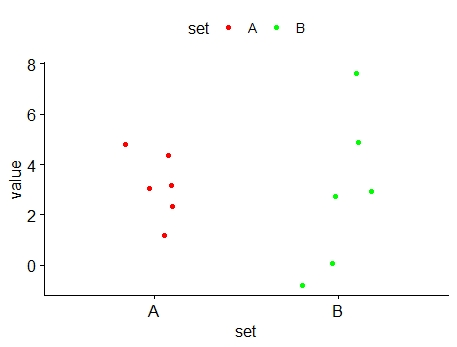
\includegraphics[width=0.5\linewidth]{images/image2_d} 

}

\caption{Scatter diagram of data sets A & B}\label{fig:d}
\end{figure}

It can be seen that, while values of data set \textbf{A} are grouped close to
their mean, while the values of data set \textbf{B} are more spread out. We
say that values of data set \textbf{B} are more dispersed (or scattered) than
those of data set \textbf{A}

This example shows that the mean, the mode and the median, are not
enough in describing a set of data. In addition to using these measures,
we need a numerical measure of dispersion (or variation) of a set of
data.

Statistical dispersion means the extent to which a numerical data is
likely to vary about an average value.

\hypertarget{characteristics-of-a-good-measure-of-dispersion}{%
\section{Characteristics of a good measure of dispersion}\label{characteristics-of-a-good-measure-of-dispersion}}

An ideal measure of dispersion is expected to possess the following
properties

\begin{enumerate}
\def\labelenumi{\arabic{enumi}.}
\item
  It should be rigidly defined
\item
  It should be based on all the items.
\item
  It should not be unduly affected by extreme items.
\item
  It should lend itself for algebraic manipulation.
\item
  It should be simple to understand and easy to calculate
\end{enumerate}

The most important measures of dispersion are the \textbf{Range}, the
\textbf{Inter-quartile range}, \textbf{Mean Absolute Deviation (MAD)}and the \textbf{standard deviation}.

\hypertarget{the-range}{%
\section{The Range}\label{the-range}}

This is the simplest possible measure of dispersion. The range of a set
of data is defined as the difference between the largest observation and
the smallest observation in the set of data.

Thus,

\textbf{Range = largest observation -- smallest observation.}

In symbols, Range = L -- S.

Where L = Largest value; S = Smallest value.

In individual observations and discrete series, L and S are easily
identified. In continuous series, the following two methods are
followed.

\hypertarget{method-1}{%
\subsection{Method 1}\label{method-1}}

L = Upper boundary of the highest class

S = Lower boundary of the lowest class.

\hypertarget{method-2}{%
\subsection{Method 2}\label{method-2}}

L = Mid-value of the highest class.

S = Mid-value of the lowest class.

\textbf{Example 5.1}: The marks obtained by 8 students in Mathematics and
Physics examinations are as follows:

Mathematics: 35, 60, 70, 40, 85, 96, 55, 65.

Physics: 50, 55, 70, 65, 89, 68, 72, 80.

Find the ranges of the two sets of data. Are the Physics marks more
dispersed than the Mathematics marks?

\textbf{Solution}

For Mathematics,

Highest mark = 96, lowest mark = 35, range =96 -- 35 = 61

For Physics,

Highest mark = 89, lowest mark = 50, range =89 -- 50 = 39.

The mathematics marks have a wider range than the Physics marks. The
Mathematics marks are therefore more dispersed than the Physics marks.

\textbf{Example 5.2}: Calculate range from the following distribution

\begin{longtable}[]{@{}llllll@{}}
\toprule
Size & 60-63 & 63-66 & 66-69 & 69-72 & 72-75 \\
\midrule
\endhead
Number & 5 & 18 & 42 & 27 & 8 \\
\bottomrule
\end{longtable}

\textbf{Solution}

L = Upper boundary of the highest class = 75

S = Lower boundary of the lowest class = 60

Range = L -- S = 75 -- 60 = 15

\hypertarget{merits-and-demerits-of-range}{%
\subsection{Merits and Demerits of Range}\label{merits-and-demerits-of-range}}

\textbf{\underline{Merits}}

\begin{enumerate}
\def\labelenumi{\arabic{enumi}.}
\item
  It is simple to understand.
\item
  It is easy to calculate.
\item
  In certain types of problems like quality control, weather
  forecasts, share price analysis, etc.
\end{enumerate}

\textbf{\underline{Demerits}}

\begin{enumerate}
\def\labelenumi{\arabic{enumi}.}
\item
  It is very much affected by the extreme items.
\item
  It is based on only two extreme observations.
\item
  It cannot be calculated from open-end class intervals.
\item
  It is not suitable for mathematical treatment.
\item
  It is a very rarely used measure.
\end{enumerate}

\hypertarget{the-inter-quartile-range-iqr-or-midspread}{%
\section{The Inter-Quartile Range (IQR) or Midspread}\label{the-inter-quartile-range-iqr-or-midspread}}

The range has the advantage that it is quick and easy to calculate.
However, since it depends only on the maximum and the minimum values of
a set of data, it does not show how the whole data is distributed
between these two values. The range is therefore not a good measure of
dispersion if one or both of these two values differ greatly from other
values of the data. To overcome this problem, we sometimes use the
inter-quartile range. A robust measure of dispersion is the
inter-quartile range. The inter-quartile range of a set of data is the
difference between the upper and lower quartiles of the data. Thus,

\textbf{Inter-Quartile Range (IQR)} = \emph{Q}\textsubscript{3} -- \emph{Q}\textsubscript{1}.

The inter-quartile range of a set of data is therefore not affected by
values of the data outside \emph{Q}\textsubscript{1} and \emph{Q}\textsubscript{3}. The inter-quartile range
is sometimes used as a measure of dispersion.

\textbf{Example 5.3}: Consider the two sets of data below, find IQR

\textbf{A}: 3, 4, 5, 6, 8, 9, 10, 12, 15

\textbf{B}: 3, 8, 8, 9, 9, 9, 10, 10, 15

For data set A, \emph{Q}\textsubscript{1} = 5, \emph{Q}\textsubscript{3} = 10; so Inter-Quartile Range =10 --
5 = 5

For data set B, \emph{Q}\textsubscript{1} = 8, \emph{Q}\textsubscript{3} = 10; so Inter-Quartile Range =10 --
8 = 2

Since the inter-quartile range of data set A is greater than that of
data set B, these results confirm that data set A is more dispersed than
data set B. You can also see Range is same for both the sets.

\hypertarget{mean-absolute-deviation-mad}{%
\section{Mean Absolute Deviation (MAD)}\label{mean-absolute-deviation-mad}}

The mean absolute deviation (MAD) is a measure of variability that
indicates the average distance between observations and their mean. MAD
uses the original units of the data, which simplifies interpretation.
Larger values signify that the data points spread out further from the
average. Conversely, lower values correspond to data points bunching
closer to it. The mean absolute deviation is also known as the mean
deviation and average absolute deviation.

Here is how to calculate the mean absolute deviation.

\begin{enumerate}
\def\labelenumi{\arabic{enumi}.}
\item
  Calculate the mean.
\item
  Calculate the difference of each observation from mean and take
  absolute value \emph{i}.\emph{e}. ignore the sign. This difference is known as
  absolute deviation
\item
  Add those deviations together.
\item
  Divide the sum by the number of data points.
\end{enumerate}

\[MAD = \frac{\sum_{i = 1}^{n}\left| x_{i} - \overline{x} \right|}{n}\]

\textbf{Example 5.4}: find the mean absolute deviation of the following 10, 15,
15, 17, 18, 21

\begin{longtable}[]{@{}llll@{}}
\toprule
Sl.No. & \(x_{i}\) & \(x_{i} - \overline{x}\) & \(\left| x_{i} - \overline{x} \right|\) \\
\midrule
\endhead
1 & 10 & -6 & 6 \\
2 & 15 & -1 & 1 \\
3 & 15 & -1 & 1 \\
4 & 17 & 1 & 1 \\
5 & 18 & 2 & 2 \\
6 & 21 & 5 & 5 \\
& \(\overline{x} =\) 16 & & \(\sum_{i = 1}^{n}\left| x_{i} - \overline{x} \right|\) = 16 \\
\bottomrule
\end{longtable}

Here n = 6 and \(\sum_{i = 1}^{n}\left| x_{i} - \overline{x} \right|\) =
16 therefore MAD = \(\frac{16}{6} = 2.67\)

\hypertarget{merits-and-demerits-of-mad}{%
\subsection{Merits and Demerits of MAD}\label{merits-and-demerits-of-mad}}

\textbf{\underline{Merits}}

\begin{enumerate}
\def\labelenumi{\arabic{enumi}.}
\item
  Simple And Easy
\item
  Different items of observations can be easily compared with mean deviation
\item
  Mean deviation is better than quartile deviation and range because it is based on all the observations of the series.
\item
  Mean deviation is less affected by the extreme values in the series while comparing to standard deviation.
\item
  Mean deviation is rigidly defined. So, it has fixed value.
\end{enumerate}

\textbf{\underline{Demerits}}

\begin{enumerate}
\def\labelenumi{\arabic{enumi}.}
\item
  It becomes difficult to compute mean deviation in case of fractions.
\item
  Mean deviation is not applicable for algebraic calculations.
\item
  It cannot be calculated from open-end class intervals.
\item
  Mean deviation is not a good measure as it ignores negative signs of deviations.
\end{enumerate}

\hypertarget{the-variance-and-standard-deviation}{%
\section{The variance and standard deviation}\label{the-variance-and-standard-deviation}}

The most important measures of variability are the sample variance and
the sample standard deviation. If \emph{x}\textsubscript{1}, \emph{x}\textsubscript{2}\ldots{} \emph{x}\textsubscript{n} is a sample
of \emph{n} observations, then the \textbf{sample variance} is denoted by \emph{s}² and
is defined by the equation.

\[{\mathbf{\text{sample variance}},\ \mathbf{s}}^{\mathbf{2}}\mathbf{=}\frac{\sum_{\mathbf{i = 1}}^{\mathbf{n}}\left( \mathbf{x}_{\mathbf{i}}\mathbf{-}\overline{\mathbf{x}} \right)^{\mathbf{2}}}{\mathbf{n - 1}}\]

The sample \textbf{standard deviation}, \emph{s}, is the positive square root of
the sample variance.

\[\mathbf{variance =}\left( \mathbf{\text{standard deviation}} \right)^{\mathbf{2}}\]

\[\mathbf{standard\ deviation = \ }\sqrt{\mathbf{\text{variance}}}\]

\textbf{Note}: If \emph{s}\textsubscript{A}, the standard deviation of data set A, is greater
than \emph{s}\textsubscript{B}, the standard deviation of data set B, then data set A is
more dispersed than data set B. It should be noted that the standard
deviation of a set of data is a non-negative number.

\textbf{Example 5.4}: Consider the two sets of data A \& B below; find standard
deviation?

\begin{longtable}[]{@{}lllllll@{}}
\toprule
\textbf{A} & 1 & 2 & 3 & 3 & 4 & 5 \\
\midrule
\endhead
\textbf{B} & -1 & 0 & 3 & 3 & 5 & 8 \\
\bottomrule
\end{longtable}

\textbf{Solution}:

\begin{longtable}[]{@{}llll@{}}
\toprule
\textbf{Set A} & & & \\
\midrule
\endhead
& \(\mathbf{x}_{\mathbf{i}}\) & \(\left( \mathbf{x}_{\mathbf{i}}\mathbf{-}\overline{\mathbf{x}} \right)\) & \(\left( \mathbf{x}_{\mathbf{i}}\mathbf{-}\overline{\mathbf{x}} \right)^{\mathbf{2}}\) \\
& 1 & -2 & 4 \\
& 2 & -1 & 1 \\
& 3 & 0 & 0 \\
& 3 & 0 & 0 \\
& 4 & 1 & 1 \\
& 5 & 2 & 4 \\
\textbf{Sum} & \textbf{18} & \textbf{0} & \textbf{10} \\
\bottomrule
\end{longtable}

Mean (\(\overline{x}\)) =\(\ \frac{18}{6} = 3\)

\[{Sample\ variane,\ s}_{A}^{2} = \frac{\sum_{i = 1}^{n}\left( x_{i} - \overline{x} \right)^{2}}{n - 1} = \frac{10}{5} = 2\]

\[\text{sample standard deviation,}\ s_{A} = \ \sqrt{s_{A}^{2}} = \ \sqrt{2} = 1.414\]

\begin{longtable}[]{@{}llll@{}}
\toprule
\textbf{Set B} & & & \\
\midrule
\endhead
& \(\mathbf{x}_{\mathbf{i}}\) & \(\left( \mathbf{x}_{\mathbf{i}}\mathbf{-}\overline{\mathbf{x}} \right)\) & \(\left( \mathbf{x}_{\mathbf{i}}\mathbf{-}\overline{\mathbf{x}} \right)^{\mathbf{2}}\) \\
& -1 & -4 & 16 \\
& 0 & -3 & 9 \\
& 3 & 0 & 0 \\
& 3 & 0 & 0 \\
& 5 & 2 & 4 \\
& 8 & 5 & 25 \\
\textbf{Sum} & \textbf{18} & \textbf{0} & \textbf{54} \\
\bottomrule
\end{longtable}

Mean (\(\overline{x}\)) =\(\ \frac{18}{6} = 3\)

\[{Sample\ variane,\ s}_{B}^{2} = \frac{\sum_{i = 1}^{n}\left( x_{i} - \overline{x} \right)^{2}}{n - 1} = \frac{54}{5} = 10.8\]

\[sample\ standard\ deviation,\ s_{B} = \ \sqrt{s_{B}^{2}} = \ \sqrt{10.8} = 3.29\]

It can be seen that \(s_{B} > s_{A}\ \), confirming that data set B is
more dispersed than data set A (see the dot diagrams)

\begin{quote}
\textbf{Note}: The unit of measurement of the sample variance is the square
of the unit of measurement of the data. Sample standard deviation has
same unit of measurement as of the data. Thus, if \emph{x} is measured in
centimetres (cm), then the unit of measurement of the sample variance is
cm\textsuperscript{2} and that of sample standard deviation is cm. The standard
deviation has the desirable property of measuring variability in the
same unit as the data.
\end{quote}

\textbf{An alternative formula for computing the variance}

The computation of \emph{s}² requires calculations of \(\overline{x}\), \emph{n}
subtractions and \emph{n} squaring and adding operations. If the original
observations or the deviations \(\left( x_{i} - \overline{x} \right)\) are
not integers, the deviations \(\left( x_{i} - \overline{x} \right)\) may
be difficult to work with, and several decimals may have to be carried
to ensure numerical accuracy. A more efficient computational formula for
\emph{s}² is given by

\(s^{2} = \frac{1}{n - 1}\left\{ \sum_{i = 1}^{n}{x_{i}^{2} - \frac{1}{n}}\left( \sum_{i = 1}^{n}x_{i} \right)^{2} \right\}\)

\textbf{Example 5.5}: Consider the data set below; find standard deviation?

\begin{longtable}[]{@{}lllllllll@{}}
\toprule
\endhead
3 & 4 & 5 & 6 & 8 & 9 & 10 & 12 & 15 \\
\bottomrule
\end{longtable}

\textbf{Solution}:

\begin{longtable}[]{@{}lll@{}}
\toprule
& \(\mathbf{x}_{\mathbf{i}}\) & \(\mathbf{x}_{\mathbf{i}}^{\mathbf{2}}\) \\
\midrule
\endhead
& 3 & 9 \\
& 4 & 16 \\
& 5 & 25 \\
& 6 & 36 \\
& 8 & 64 \\
& 9 & 81 \\
& 10 & 100 \\
& 12 & 144 \\
& 15 & 225 \\
\textbf{Sum} & \textbf{72} & \textbf{700} \\
\bottomrule
\end{longtable}

\(s^{2} = \frac{1}{n - 1}\left\{ \sum_{i = 1}^{n}{x_{i}^{2} - \frac{1}{n}}\left( \sum_{i = 1}^{n}x_{i} \right)^{2} \right\}\)
; here \emph{n} = 9

\(s^{2} = \frac{1}{8}\left\{ 700 - {\frac{1}{9}\left( 72 \right)}^{2} \right\}\)
=15.5

\(s = \ \sqrt{15.5} = 3.94\)

\hypertarget{variance-and-standard-deviation-for-grouped-data}{%
\subsection{Variance and standard deviation for grouped data}\label{variance-and-standard-deviation-for-grouped-data}}

\hypertarget{for-discrete-grouped-data}{%
\subsubsection{For discrete grouped data}\label{for-discrete-grouped-data}}

\[s^{2} = \frac{1}{n - 1}\left\{ \sum_{i = 1}^{n}{{f_{i}x}_{i}^{2} - \frac{1}{n}}\left( \sum_{i = 1}^{n}{f_{i}x}_{i} \right)^{2} \right\}\]

where \(f_{i}\) is the frequency of \emph{i}\textsuperscript{th} observation

\textbf{Example 5.6}: The frequency distributions of seed yield of 50 sesamum
plants are given below. Find the standard deviation.

\begin{longtable}[]{@{}llllll@{}}
\toprule
Seed yield in gms (\emph{x}) & \textbf{3} & \textbf{4} & \textbf{5} & \textbf{6} & \textbf{7} \\
\midrule
\endhead
Frequency (\emph{f}) & \textbf{4} & \textbf{6} & \textbf{15} & \textbf{15} & \textbf{10} \\
\bottomrule
\end{longtable}

\textbf{Solution}:

\begin{longtable}[]{@{}llll@{}}
\toprule
\textbf{\emph{x}} & \textbf{\emph{f}} & \textbf{\emph{fx}} & \textbf{\emph{fx\textsuperscript{2}}} \\
\midrule
\endhead
3 & 4 & 12 & 36 \\
4 & 6 & 24 & 96 \\
5 & 15 & 75 & 375 \\
6 & 15 & 90 & 540 \\
7 & 10 & 70 & 490 \\
\textbf{Total} & \textbf{50} & \textbf{271} & \textbf{1537} \\
\bottomrule
\end{longtable}

\[s^{2} = \frac{1}{n - 1}\left\{ \sum_{i = 1}^{n}{{f_{i}x}_{i}^{2} - \frac{1}{n}}\left( \sum_{i = 1}^{n}{f_{i}x}_{i} \right)^{2} \right\}\]

\[{sample\ variance,\ s}^{2} = \frac{1}{50 - 1}\left\{ 1537 - \frac{271^{2}}{50} \right\} = 1.3914\]

\(standard\ deviation,\ s = \sqrt{1.3914}\) = 1.179

\hypertarget{for-continuous-grouped-data}{%
\subsubsection{For continuous grouped data}\label{for-continuous-grouped-data}}

\[s^{2} = \frac{1}{n - 1}\left\{ \sum_{i = 1}^{n}{{f_{i}d}_{i}^{2} - \frac{1}{n}}\left( \sum_{i = 1}^{n}{f_{i}d}_{i} \right)^{2} \right\}\]

where \(f_{i}\) is the frequency of \emph{i}\textsuperscript{th} class, \emph{c} is the class
interval, \(d_{i} = \frac{x_{i} - A}{c}\), \(x_{i}\) is the class mark, \(A\)
is the class mark with the highest frequency

\textbf{Example 5.7}: The frequency distributions of seed yield of 50 sesamum
plants are given below. Find the standard deviation

\begin{longtable}[]{@{}llllll@{}}
\toprule
Seed yield in gms (\emph{x}) & 2.5-3.5 & 3.5-4.5 & 4.5-5.5 & 5.5-6.5 & 6.5-7.5 \\
\midrule
\endhead
Frequency (\emph{f}) & 4 & 6 & 15 & 15 & 10 \\
\bottomrule
\end{longtable}

\textbf{Solution}:

Here \emph{n} =50; \emph{c} =1

\begin{longtable}[]{@{}llllll@{}}
\toprule
\textbf{Seed yield} & \emph{f} & \emph{x} & \(d_{i} = \frac{x_{i} - A}{c}\) & \emph{fd} & \emph{f d\textsuperscript{2}} \\
\midrule
\endhead
2.5-3.5 & 4 & 3 & -2 & -8 & 16 \\
3.5-4.5 & 6 & 4 & -1 & -6 & 6 \\
4.5-5.5 & 15 & 5 & 0 & 0 & 0 \\
6.5-7.5 & 15 & 6 & 1 & 15 & 15 \\
7.5-8.5 & 10 & 7 & 2 & 20 & 40 \\
\textbf{Total} & \textbf{50} & \textbf{25} & \textbf{0} & \textbf{21} & \textbf{77} \\
\bottomrule
\end{longtable}

\emph{A} = 5

\[s^{2} = \frac{1}{n - 1}\left\{ \sum_{i = 1}^{n}{{f_{i}d}_{i}^{2} - \frac{1}{n}}\left( \sum_{i = 1}^{n}{f_{i}d}_{i} \right)^{2} \right\}\]

\[{sample\ variance,\ s}^{2} = \frac{1}{49}\left( 77 - \frac{\left( 21 \right)^{2}}{50} \right) = \ 1.3914\]

\(standard\ deviation,\ s = \sqrt{1.3914}\) = 1.179

\hypertarget{merits-and-demerits-of-standard-deviation}{%
\subsection{Merits and Demerits of Standard Deviation}\label{merits-and-demerits-of-standard-deviation}}

\textbf{\underline{Merits}}

\begin{enumerate}
\def\labelenumi{\arabic{enumi}.}
\item
  It is rigidly defined and its value is always definite and based on
  all the observations
\item
  As it is based on arithmetic mean, it has all the merits of
  arithmetic mean.
\item
  It is the most important and widely used measure of dispersion.
\item
  It is possible for further algebraic treatment.
\item
  It is less affected by the fluctuations of sampling and hence
  stable.
\item
  It is the basis for measuring the coefficient of correlation and
  other measures.
\end{enumerate}

\textbf{\underline{Demerits}}

\begin{enumerate}
\def\labelenumi{\arabic{enumi}.}
\item
  It is not easy to understand and it is difficult to calculate.
\item
  It gives more weight to extreme values because the values are
  squared up.
\item
  As it is an absolute measure of variability, it cannot be used for
  the purpose of comparison.
\end{enumerate}

\hypertarget{coefficient-of-variation-relative-measure-of-dispersion}{%
\section{Coefficient of Variation (relative measure of dispersion)}\label{coefficient-of-variation-relative-measure-of-dispersion}}

The Standard deviation is an absolute measure of dispersion. It is
expressed in terms of units in which the original figures are collected
and stated. The standard deviation of heights of plants cannot be
compared with the standard deviation of weights of the grains, as both
are expressed in different units, \emph{i}.\emph{e} heights in centimetre and
weights in kilograms.

Therefore the standard deviation must be converted into a relative
measure of dispersion for the purpose of comparison. The relative
measure is known as the \textbf{coefficient of variation}. The coefficient of
variation is obtained by dividing the standard deviation by the mean and
expressed in percentage.

\[\mathbf{\text{Coefficient of variation}}\left( \mathbf{C}\mathbf{.}\mathbf{V} \right)\mathbf{=}\frac{\mathbf{\text{standard deviation}}}{\mathbf{\text{mean}}}\mathbf{\times 100}\]

If we want to compare the variability of two or more series, we can use
C.V. The series or groups of data for which the C.V. is greater indicate
that the group is more variable, less stable, less uniform, less
consistent or less homogeneous. If the C.V. is less, it indicates that
the group is less variable or more stable or more uniform or more
consistent or more homogeneous.

\textbf{Example 5.8}: Consider the measurement on yield and plant height of a
paddy variety. The mean and standard deviation for yield are 50 kg and
10 kg respectively. The mean and standard deviation for plant height are
55 cm and 5 cm respectively. Compare the variability.

\textbf{Solution}:

Here the measurements for yield and plant height are in different units.
Hence the variability can be compared only by using coefficient of
variation.

For yield, CV=\(\ \frac{10}{50} \times 100 =\) 20\%

For plant height, CV=
\(\frac{5}{55} \times 100 = \ \)9.1\%

The yield is subject to more variation than the plant height.

\textbf{******************************************************************}

\hypertarget{skewness-and-kurtosis}{%
\chapter{Skewness and Kurtosis}\label{skewness-and-kurtosis}}

In the previous lectures we have learned numerical measures of central
tendency and dispersion, but what about measures of shape?

The histogram can give you a general idea on the shape of the
distribution of values in your data. But we need some numerical measures
to identify the shape of the distribution. The numerical measures which
deal with the shape of the distribution are Skewness and Kurtosis.

\hypertarget{skewness}{%
\section{Skewness}\label{skewness}}

Skewness is a measure of symmetry, or more precisely, the lack of
symmetry. Then you may ask, what will a symmetric distribution looks
like. Histogram of a symmetric distribution is showed below:

\begin{figure}

{\centering 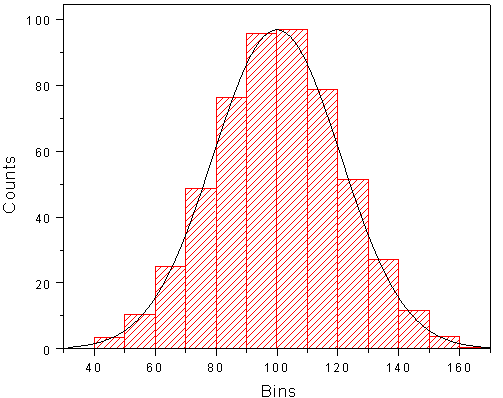
\includegraphics[width=0.5\linewidth]{images/Hist1} 

}

\caption{Histogram of a symmetric distribution}\label{fig:hs}
\end{figure}

A distribution, or data set, is symmetric if it looks the same to the
left and right of the centre point. In our discussion we are including
only unimodal cases.

For a symmetric distribution skewness = 0; mean = median = mode

\begin{figure}

{\centering 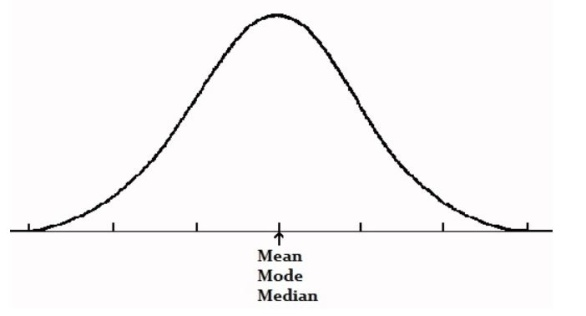
\includegraphics[width=0.5\linewidth]{images/image3_5} 

}

\caption{symmetric distribution}\label{fig:hs1}
\end{figure}

Example of a data set with skewness = 0 (symmetric distribution)

\begin{figure}

{\centering 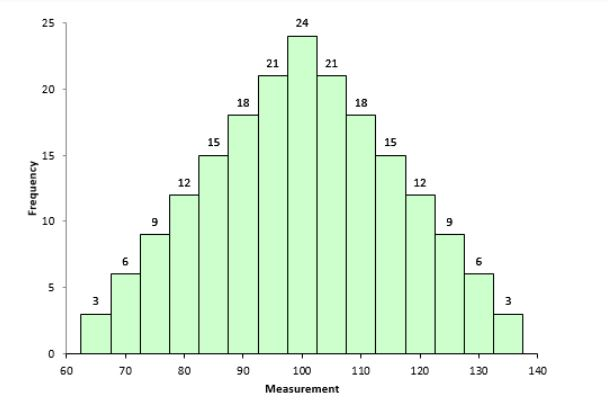
\includegraphics[width=0.5\linewidth]{images/image4_5} 

}

\caption{Data set with skewness = 0}\label{fig:sk0}
\end{figure}

\hypertarget{left-skewed-or-negatively-skewed}{%
\subsection{Left-skewed or negatively skewed}\label{left-skewed-or-negatively-skewed}}

For negatively skewed data set or distribution, the left tail is longer;
the mass of the distribution is concentrated on the right of the figure.
The distribution is said to be left-skewed, left-tailed, or skewed to
the left, considering that there is a long tail in the left side. See
the figure below, you can also see Mean \textless{} Median \textless{} Mode.

\begin{figure}

{\centering 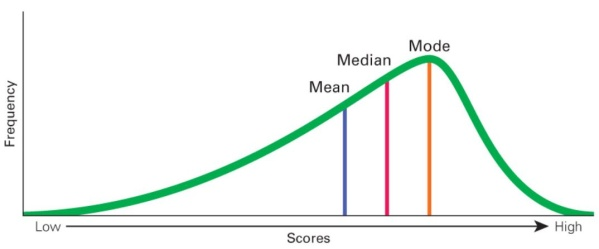
\includegraphics[width=0.5\linewidth]{images/image5_5} 

}

\caption{Left skewed or negatively skewed distribution}\label{fig:sk1}
\end{figure}

Example of a data set with negative skewness

\begin{figure}

{\centering 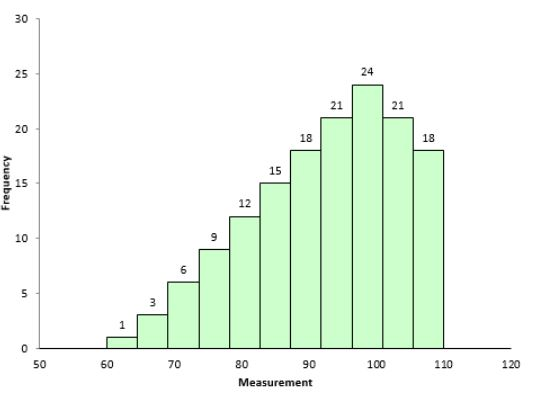
\includegraphics[width=0.5\linewidth]{images/image6_5} 

}

\caption{Negatively skewed data set}\label{fig:sk3}
\end{figure}

\hypertarget{right-skewed-or-positively-skewed}{%
\subsection{Right-skewed or positively skewed}\label{right-skewed-or-positively-skewed}}

For positively skewed data set or distribution, the right tail is
longer; the mass of the distribution is concentrated on the left of the
figure. The distribution is said to be right-skewed, right-tailed, or
skewed to the right, considering that there is a long tail in the right
side. See the figure below, you can also see Mean \textgreater{} Median \textgreater{} Mode

\begin{figure}

{\centering 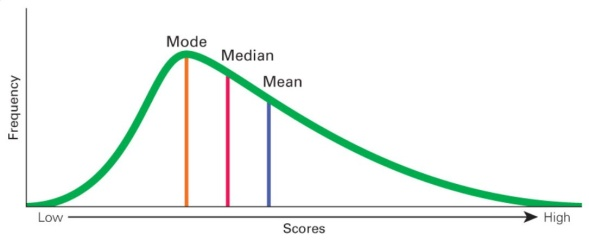
\includegraphics[width=0.5\linewidth]{images/image7_5} 

}

\caption{Right skewed or positively skewed distribution}\label{fig:sk4}
\end{figure}

Example of a data set with positive skewness

\begin{figure}

{\centering 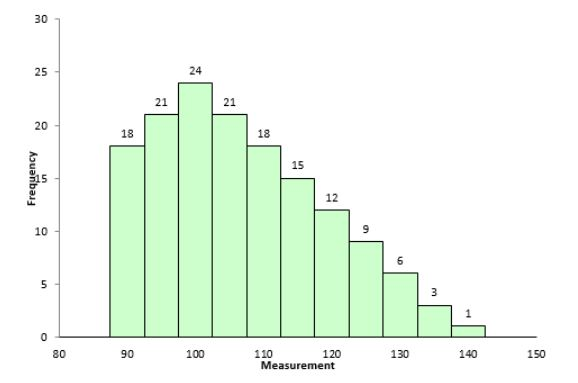
\includegraphics[width=0.5\linewidth]{images/image8_5} 

}

\caption{Data set with positive skewness (right skewed)}\label{fig:sk5}
\end{figure}

\hypertarget{measures-of-skewness}{%
\section{Measures of Skewness}\label{measures-of-skewness}}

The direction and extent of skewness can be measured in various ways. We
shall discuss four measures.

\hypertarget{karl-pearsons-coefficient-of-skewness-s_k}{%
\subsection{\texorpdfstring{Karl Pearson's coefficient of Skewness (\textbf{\(S_{k}\)})}{Karl Pearson's coefficient of Skewness (S\_\{k\})}}\label{karl-pearsons-coefficient-of-skewness-s_k}}

You have noticed that the mean, median and mode are not equal in a
skewed distribution. The Karl Pearson's measure of skewness is based
upon the divergence of mean from mode in a skewed distribution.

\[S_{k} = \frac{mean - mode}{\text{standard deviation}}\]

The sign of \(S_{k}\) gives the direction of skewness and its magnitude
gives the extent of skewness. If \(S_{k}\) \textgreater{} 0, the distribution is
positively skewed, and if \(S_{k}\) \textless{} 0 it is negatively skewed.

In the above formula since mode is used, there is a problem that if mode
is not defined for a distribution we cannot find \(S_{k}\). But empirical
relation between mean, median and mode states that, for a moderately
symmetrical distribution\(\ mean - mode \approx 3(mean - median)\). So the
above formula can be written as

\[S_{k} = \frac{3(mean - median)}{\text{standard deviation}}\]

\textbf{Example 6.1}: Compute the Karl Pearson's coefficient of skewness from
the following data:

\begin{longtable}[]{@{}ll@{}}
\toprule
Height (\emph{x}) & frequency (\emph{f}) \\
\midrule
\endhead
58 & 10 \\
59 & 18 \\
60 & 30 \\
61 & 42 \\
62 & 35 \\
63 & 28 \\
64 & 16 \\
65 & 8 \\
\bottomrule
\end{longtable}

Solution:

\begin{longtable}[]{@{}llll@{}}
\toprule
Height (\(x_{i}\)) & frequency (\(f_{i}\)) & \(f_{i}x_{i}\) & \(f_{i}x_{i}^{2}\) \\
\midrule
\endhead
58 & 10 & 580 & 33640 \\
59 & 18 & 1062 & 62658 \\
60 & 30 & 1800 & 108000 \\
61 & 42 & 2562 & 156282 \\
62 & 35 & 2170 & 134540 \\
63 & 28 & 1764 & 111132 \\
64 & 16 & 1024 & 65536 \\
65 & 8 & 520 & 33800 \\
\textbf{Sum} & \textbf{187} & \textbf{11482} & \textbf{705588} \\
\bottomrule
\end{longtable}

Mean,
\(\overline{x} = \frac{\sum_{i = 1}^{n}{f_{i}x_{i}}}{\sum_{i = 1}^{n}f_{i}}\)
= \(\frac{11482}{187} = 61.40\)

\({sample\ variance,\ s}^{2} = \frac{1}{n - 1}\left\{ \sum_{i = 1}^{n}{{f_{i}x}_{i}^{2} - \frac{1}{n}}\left( \sum_{i = 1}^{n}{f_{i}x}_{i} \right)^{2} \right\}\)=
\(\frac{705588 - \frac{\left( 11482 \right)^{2}}{187}}{186} = 3.123\)

\(standard\ deviation,\ s = \sqrt{3.123} = 1.179\)

Median: See in the cumulative frequencies, the value just greater
than\(\ \left( \frac{n + 1}{2} \right)\) , then the corresponding value of
\(x\) is \(Q_{2}\), median

\(\left( \frac{n + 1}{2} \right) = \frac{187 + 1}{2}\ \)= \(\frac{188}{2}\)
= 94

\begin{longtable}[]{@{}lll@{}}
\toprule
Height (\emph{x}) & frequency (\emph{f}) & cumulative frequency \\
\midrule
\endhead
58 & 10 & 10 \\
59 & 18 & 28 \\
60 & 30 & 58 \\
61 & 42 & 100 \\
62 & 35 & 135 \\
63 & 28 & 163 \\
64 & 16 & 179 \\
65 & 8 & 187 \\
\bottomrule
\end{longtable}

\[S_{k} = \frac{3(mean - median)}{\text{standard deviation}}\]

\[S_{k} = \frac{3(61.40 - 61)}{1.179} = \frac{1.2}{1.179} = 1.017\]

Hence, the Karl Pearson's coefficient of skewness \(S_{k}\)=\(1.017\), Thus
the distribution is positively skewed.

\hypertarget{bowleys-measure-of-skewness-sq}{%
\subsection{\texorpdfstring{Bowley's measure of Skewness (\emph{S}\textsubscript{Q})}{Bowley's measure of Skewness (SQ)}}\label{bowleys-measure-of-skewness-sq}}

Karl Pearson's coefficient of skewness is most commonly used skewness
measure. However, in order to use it you must know the mean, mode (or
median) and standard deviation for your data. Sometimes you might not
have that information; instead you might have information about
quartiles. If that's the case, you can use Bowley's measure of Skewness
as an alternative to find out more about the asymmetry of your
distribution. It's very useful if you have extreme data values
(outliers) or if you have an open-ended distribution.

\[{Bowley’s\ measure\ of\ Skewness,\ S}_{Q} = \frac{\left( Q_{3} - Q_{2} \right) - \left( Q_{2} - Q_{1} \right)}{\left( Q_{3} - Q_{2} \right) + \left( Q_{2} - Q_{1} \right)}\]

Where \(Q_{1}\)= 1\textsuperscript{st} quartile; \(Q_{2}\) = median; \(Q_{3}\)= 3\textsuperscript{rd} quartile

Equation can be further modified into

\[S_{Q} = \frac{Q_{3} - 2Q_{2} + Q_{1}}{Q_{3} - Q_{1}}\]

\begin{itemize}
\item
  \(S_{Q}\)= 0 means that the curve is symmetrical.
\item
  \(S_{Q}\) \textgreater{} 0 means the curve is positively skewed.
\item
  \(S_{Q}\)\textless{} 0 means the curve is negatively skewed.
\end{itemize}

For \textbf{Example 6.1} given above, Bowley's measure of Skewness can be
calculated as follows

\begin{longtable}[]{@{}lll@{}}
\toprule
Height (\emph{x}) & frequency (\emph{f}) & cumulative frequency \\
\midrule
\endhead
58 & 10 & 10 \\
59 & 18 & 28 \\
60 & 30 & 58 \\
61 & 42 & 100 \\
62 & 35 & 135 \\
63 & 28 & 163 \\
64 & 16 & 179 \\
65 & 8 & 187 \\
\bottomrule
\end{longtable}

Calculation of\(\text{Q}_{1}\), \(Q_{2}\), \(Q_{3}\) is given in Section \ref{quartile}

\[{Q}_{1} = 60\]

\[Q_{2} = 61\]

\[Q_{3} = 63\]

\[S_{Q} = \frac{63 - (2 \times 61) + 60}{63 - 60} = \ \frac{1}{3} = 0.33\]

Since \(S_{Q}\) \textgreater{} 0 means the curve is positively skewed.

\hypertarget{kellys-measure-of-skewness-sp}{%
\subsection{\texorpdfstring{Kelly's Measure of Skewness (\emph{S}\textsubscript{p})}{Kelly's Measure of Skewness (Sp)}}\label{kellys-measure-of-skewness-sp}}

Bowley's measure of skewness is based on the middle 50\% of the
observations; it leaves 25\% of the observations on each extreme of the
distribution. As an improvement over Bowley's measure, Kelly has
suggested a measure based on Percentiles, including \emph{P}\textsubscript{10} and \emph{P}\textsubscript{90}
so that only 10\% of the observations on each extreme are ignored.

\[{Kelly's\ Measure\ of\ Skewness,\ S}_{p} = \frac{\left( P_{90} - P_{50} \right) - \left( P_{50} - P_{10} \right)}{\left( P_{90} - P_{50} \right) + \left( P_{50} - P_{10} \right)}\]

\begin{rmdnote}
Assignment 3:Try to find Kelly's Measure of Skewness
for the Example 6.1 given above
\end{rmdnote}

\hypertarget{measure-based-on-moments}{%
\subsection{Measure based on moments}\label{measure-based-on-moments}}

Before going into measuring skewness using moments, one should know what
a moment is:

\hypertarget{moments}{%
\subsubsection{Moments}\label{moments}}

The \textbf{\emph{r}\textsuperscript{th} moment about mean} of a distribution, denoted by
\textbf{\emph{μ}\textsubscript{r}} is given by

\[\mu_{r} = \frac{\sum_{i = 1}^{N}{f_{i}\left( x_{i} - \overline{x} \right)^{r}}}{N}\]

Where \(f_{i}\) is the frequency of \emph{i}\textsuperscript{th} observation or class
mark\(\ x_{i}\), \(N = \sum_{}^{}f_{i}\), number of observations

Moment about mean is also called as \textbf{Central Moment}

If \emph{r} = 0,
\(\mu_{0} = \frac{\sum_{i = 1}^{N}{f_{i}\left( x_{i} - \overline{x} \right)^{0}}}{N}\)
= 1

If \emph{r} = 1,
\(\mu_{1} = \frac{\sum_{i = 1}^{N}{f_{i}\left( x_{i} - \overline{x} \right)^{1}}}{N}\)
= 0 (sum of deviation about mean is zero)

If \emph{r} = 2,
\(\mu_{2} = \frac{\sum_{i = 1}^{N}{f_{i}\left( x_{i} - \overline{x} \right)^{2}}}{N}\)
= \(\sigma^{2}\), Population variance

In short values of following moments about mean are

\begin{longtable}[]{@{}
  >{\raggedright\arraybackslash}p{(\columnwidth - 2\tabcolsep) * \real{0.35}}
  >{\raggedright\arraybackslash}p{(\columnwidth - 2\tabcolsep) * \real{0.24}}@{}}
\toprule
\textbf{Moments about mean}

\textbf{(central moment)} & \textbf{Value} \\
\midrule
\endhead
\(\mu_{0}\) & 1 \\
\(\mu_{1}\) & 0 \\
\(\mu_{2}\) & \(\sigma^{2}\) \\
\bottomrule
\end{longtable}

For the \textbf{Example 6.1} given above, calculate third central moment, \(\mu_{3}\)

\begin{longtable}[]{@{}llll@{}}
\toprule
Height (\(x_{i}\)) & frequency (\(f_{i}\)) & \(\left( x_{i} - \overline{x} \right)^{3}\) & \({f_{i}\left( x_{i} - \overline{x} \right)}^{3}\) \\
\midrule
\endhead
58 & 10 & -39.304 & -393.04 \\
59 & 18 & -13.824 & -248.832 \\
60 & 30 & -2.744 & -82.32 \\
61 & 42 & -0.064 & -2.688 \\
62 & 35 & 0.216 & 7.56 \\
63 & 28 & 4.096 & 114.688 \\
64 & 16 & 17.576 & 281.216 \\
65 & 8 & 46.656 & 373.248 \\
\textbf{Sum} & \textbf{187} & \textbf{~} & \textbf{49.832} \\
\bottomrule
\end{longtable}

Mean = 61.40

\[\mu_{3} = \frac{\sum_{i = 1}^{N}{f_{i}\left( x_{i} - \overline{x} \right)^{3}}}{N} = \ \frac{49.832}{187} = 0.266\]

\hypertarget{moment-measure-of-skewness-mathbfbeta_1textandgamma_1mathbf}{%
\subsubsection{\texorpdfstring{Moment Measure of Skewness \(\mathbf{(}\beta_{1}\text{and}\)\(\gamma_{1}\mathbf{)}\)}{Moment Measure of Skewness \textbackslash mathbf\{(\}\textbackslash beta\_\{1\}\textbackslash text\{and\}\textbackslash gamma\_\{1\}\textbackslash mathbf\{)\}}}\label{moment-measure-of-skewness-mathbfbeta_1textandgamma_1mathbf}}

The moment measure of skewness is based on the property that, for a
symmetrical distribution, all odd ordered central moments are equal to
zero. We note that \(\mu_{1}\) = 0, for every distribution, therefore, the
lowest order moment that can provide an absolute measure of skewness
is\(\text{μ}_{3}\). So measures of skewness are based
on\(\text{μ}_{3}\).

\[\beta_{1} = \frac{\mu_{3}^{2}}{\mu_{2}^{3}}\]

Pronounced as `beta one'

\(\beta_{1}\)= 0 means that the curve is symmetrical. The greater the
value of \(\beta_{1}\)the more skewed the distribution. One serious
limitation of \(\beta_{1}\)is that it cannot tell the direction of
skewness, \emph{i}.\emph{e}., whether it is positive or negative. Since
\(\text{μ}_{2}\) is always positive and \(\mu_{3}^{2}\) is positive,
\(\beta_{1}\) will be positive always. This drawback is removed by
calculating\(\text{γ}_{1}\), called as Karl Pearson's\(\text{ γ}_{1}\),
pronounced as `gamma one'.

\[\gamma_{1} = \sqrt{\beta_{1}} = \frac{\mu_{3}}{\mu_{2}^{3}}\]

If \(\mu_{3}\) is positive \(\gamma_{1}\) is positive, If \(\mu_{3}\) is
negative \(\gamma_{1}\) is negative

\begin{itemize}
\item
  \(\gamma_{1}\)= 0 means that the curve is symmetrical.
\item
  \(\gamma_{1}\) \textgreater{} 0 means the curve is positively skewed.
\item
  \(\gamma_{1}\)\textless{} 0 means the curve is negatively skewed.
\end{itemize}

For the \textbf{Example 6.1} given above, skewness can be examined as below

\(\mu_{3}\)= 0.226

\(\mu_{2}\)= 3.123

\(\beta_{1} = \frac{\mu_{3}^{2}}{\mu_{2}^{3}}\) =
\(\frac{\left( 0.226 \right)^{2}}{\left( 3.123 \right)^{3}} = \ \frac{0.051}{30.46} = 0.0016\)

\(\gamma_{1} = \sqrt{\beta_{1}} = \ \sqrt{0.0016} = + 0.04\)

Since \(\mu_{3}\) is positive \(\gamma_{1}\)is positive. Since
\(\gamma_{1}\)is slightly greater than 0, distribution is a slightly
skewed to right.

\hypertarget{kurtosis}{%
\section{Kurtosis}\label{kurtosis}}

Kurtosis is another measure of the shape of a distribution. Whereas
skewness measures the lack of symmetry of the frequency curve of a
distribution, kurtosis is a measure of the relative peakedness of its
frequency curve. Various frequency curves can be divided into three
categories depending upon the shape of their peak.

\begin{figure}

{\centering 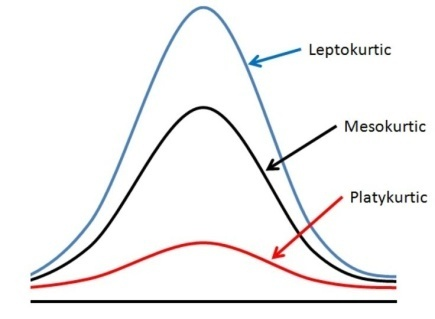
\includegraphics[width=0.5\linewidth]{images/image10_5} 

}

\caption{Three categories of frequency curves depending upon the shape of their peak}\label{fig:k1}
\end{figure}

Kurtosis refers to degree of flatness or peakedness of the curve. It is
measured relative to the peakedness of normal curve. The normal curve is considered as \emph{mesokurtic}. If a curve is
more peaked than normal curve, it is called \emph{leptokurtic}. If a curve is
more flat-topped than normal curve, it is called \emph{platykurtic}.

The condition of peakedness (leptokurtic) or flatness (platykurtic) is
called \textbf{kurtosis of excess}.

Measure of kurtosis is given by `beta two' given by Karl Pearson

\(\beta_{2} = \frac{\mu_{4}}{\mu_{2}^{2}}\)

Where \(\mu_{4}\) is the 4\textsuperscript{th} central moment, \(\mu_{2}\) is the 2\textsuperscript{nd}
central moment

\begin{itemize}
\item
  \(\beta_{2}\)= 3 means that the curve is mesokurtic.
\item
  \(\beta_{2}\) \textgreater{} 3 means the curve is leptokurtic.
\item
  \(\beta_{2}\)\textless{} 3 means the curve is platykurtic.
\end{itemize}

Another measure of kurtosis is gamma two, \(\gamma_{2} = \beta_{2} - 3\ \)

\begin{itemize}
\item
  \(\gamma_{2}\)= 0 means that the curve is mesokurtic.
\item
  \(\gamma_{2}\) \textgreater{} 0 means the curve is leptokurtic.
\item
  \(\gamma_{2}\)\textless{} 0 means the curve is platykurtic.
\end{itemize}

For the \textbf{Example 6.1} given above, kurtosis can be examined as follows

\begin{longtable}[]{@{}llll@{}}
\toprule
Height (\(x_{i}\)) & frequency (\(f_{i}\)) & \(\left( x_{i} - \overline{x} \right)^{4}\) & \({f_{i}\left( x_{i} - \overline{x} \right)}^{4}\) \\
\midrule
\endhead
58 & 10 & 133.6336 & 1336.336 \\
59 & 18 & 33.1776 & 597.1968 \\
60 & 30 & 3.8416 & 115.248 \\
61 & 42 & 0.0256 & 1.0752 \\
62 & 35 & 0.1296 & 4.536 \\
63 & 28 & 6.5536 & 183.5008 \\
64 & 16 & 45.6976 & 731.1616 \\
65 & 8 & 167.9616 & 1343.693 \\
\textbf{Sum} & \textbf{187} & & \textbf{4312.747} \\
\bottomrule
\end{longtable}

Mean,\(\ \overline{x}\ \)= 61.40

\(\mu_{2}\) = 3.123 (calculation shown in previous example)

\(\mu_{4} = \frac{\sum_{i = 1}^{N}{f_{i}\left( x_{i} - \overline{x} \right)^{4}}}{N} = \frac{4312.747}{187} = 23.062\)

\(\beta_{2} = \frac{\mu_{4}}{\mu_{2}^{2}} = \frac{23.062}{\left( 3.123 \right)^{2}} = 2.364\)

\(\beta_{2}\) is 2.364, which is close to 3, distribution can be considered
slightly platykurtic close to symmetric.

You can verify the frequency curve of \textbf{Example 6.1} below, it can be seen
that it is slightly right tailed (positively skewed)

\begin{figure}

{\centering 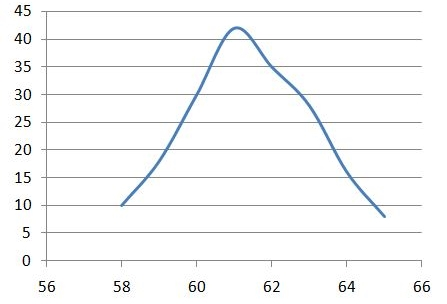
\includegraphics[width=0.5\linewidth]{images/image11_5} 

}

\caption{frequency curve of Example 6.1}\label{fig:k2}
\end{figure}

\hypertarget{measures-of-association}{%
\chapter{Measures of Association}\label{measures-of-association}}

\hypertarget{scatter-diagram}{%
\section{Scatter Diagram}\label{scatter-diagram}}

Consider two variables \emph{x} and \emph{y}, we use scatter diagram to
investigate whether there is any relation between the two variables. If
the variables \emph{x} and \emph{y} are plotted along the X-axis and Y-axis
respectively in the X-Y plane of a graph sheet the resultant diagram of
dots is known as \textbf{scatter diagram}. From the scatter diagram we can
say whether there is any association between X and Y.

\textbf{Example 7.1}: Consider the data on Sepal length (\emph{x}) and Sepal width (\emph{y}) of \emph{Iris} \emph{setosa.}

\begin{longtable}[]{@{}lll@{}}
\toprule
Sl. No.~ & Sepal Length & Sepal Width \\
\midrule
\endhead
1 & 5.1 & 3.5 \\
2 & 4.9 & 3 \\
3 & 4.7 & 3.2 \\
4 & 4.6 & 3.1 \\
5 & 5 & 3.6 \\
6 & 7 & 3.2 \\
7 & 6.4 & 3.2 \\
8 & 6.9 & 3.1 \\
9 & 5.5 & 2.3 \\
10 & 6.5 & 2.8 \\
11 & 6.3 & 3.3 \\
12 & 5.8 & 2.7 \\
13 & 7.1 & 3 \\
14 & 6.3 & 2.9 \\
15 & 6.5 & 3 \\
\bottomrule
\end{longtable}

\begin{figure}

{\centering 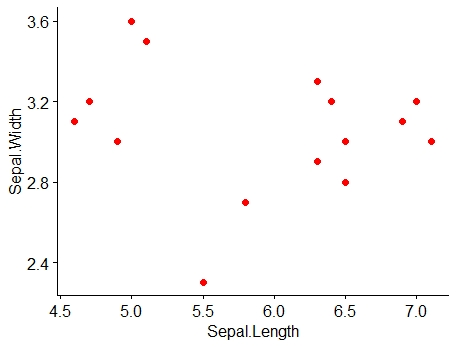
\includegraphics[width=0.5\linewidth]{images/image2c} 

}

\caption{Scatter diagram of data in Example 7.1}\label{fig:c1}
\end{figure}

\hypertarget{correlation}{%
\section{Correlation}\label{correlation}}

Correlation is a statistical technique used for analyzing the behaviour
of two or more variables. The correlation measures the degree and
closeness of the linear relationship between two variables in
numerical magnitude.

Correlation measure will enable us to compare the linear relationship
between two variables by using a single number. If two or more
quantities vary in a related manner so that the movements in one tend to
be accompanied by the movements in the other, then they are said to be
correlated.

\hypertarget{positive-correlation}{%
\subsection{Positive correlation}\label{positive-correlation}}

Positive correlation is a relationship between two variables in
which both variables move in the same direction. A positive correlation
exists when one variable decreases as the other variable decreases, or
one variable increases while the other increases.

Examples of positive correlation: consider two variables \emph{x} and \emph{y}

\begin{itemize}
\item
  The more time you spend running on a treadmill {[}Running time
  (\emph{x}){]}, the more calories you will burn {[}calories burned (\emph{y}){]}.
  Here you can see as \emph{x} increases \emph{y} also increases
\item
  Shorter people {[}Height (\emph{x}){]} have smaller shoe sizes {[}shoe size
  (\emph{y}){]}. Here you can see as \emph{x} decreases \emph{y} also decreases.
\item
  The more hours you spend in direct sunlight {[}Hours in sunlight
  (\emph{x}){]}, the more is your tan {[}melanin content(\emph{y}){]}. Here you can
  see as \emph{x} increases \emph{y} also increases
\item
  As the temperature goes up {[}Temperature (\emph{x}){]}, ice cream sales
  {[}sales (\emph{y}){]}, also go up.
\end{itemize}

\hypertarget{negative-correlation}{%
\subsection{Negative correlation}\label{negative-correlation}}

Negative correlation is a relationship between two variables in
which one variable increases as the other decreases, and vice versa.

Examples of negative correlation: consider two variables \emph{x} and \emph{y}

\begin{itemize}
\item
  A student who has many absences {[}No.~of days absent (\emph{x}){]} has a
  decrease in grades {[}grades (\emph{x}){]}. Here you can see as \emph{x}
  increases \emph{y} decreases.
\item
  As weather gets colder {[}Average monthly temperature (\emph{x}){]}, air
  conditioning costs decrease {[}Price of A.C (\emph{y}){]}.
\item
  If a chicken increases in age {[}chicken age (\emph{x}){]}, the number of
  eggs it produces {[}No.~of eggs produced (\emph{y}){]} decreases.
\item
  If a car decreases speed {[}average car speed(\emph{x}){]}, travel time
  (\emph{y}) to a destination increases.
\end{itemize}

\hypertarget{other-types-of-correlation}{%
\section{Other types of correlation}\label{other-types-of-correlation}}

\hypertarget{simple-and-multiple}{%
\subsection{Simple and Multiple}\label{simple-and-multiple}}

In \underline{simple correlation} the relationship
is confined to two variables only. In \underline{multiple correlation} the
relationship between more than two variables is judged.

\hypertarget{partial-and-total}{%
\subsection{Partial and total}\label{partial-and-total}}

There are two types of correlations in multiple
correlation analysis.

Under \underline{partial correlation} the relationship of two or variables is
examined after eliminating the linear effect of other correlated
variables.

The \underline{total correlation} is based on all relevant variables.

\begin{quote}
Correlation measures only linear relationship between variables
\end{quote}

\hypertarget{linear-relationship}{%
\section{Linear relationship}\label{linear-relationship}}

A linear relationship (or linear association)
is a statistical term used to describe a straight-line relationship
between variables.

Linear relationships can be expressed either in a graphical format where
the variable plotted on X-Y plane gives a straight line or relation
between two variables (consider \emph{x} and \emph{y}) can be expressed with an
equation of a straight line (\emph{y} = \emph{a} + \emph{bx}) (**will be more clear
when we discuss regression)

\textbf{Example 7.2}: Consider the following example of ice cream sales

The local ice cream shop keeps track of how much ice cream they sell
versus the temperature on that day; here are their figures for the last
12 days:

\begin{longtable}[]{@{}ll@{}}
\toprule
Temperature (°C) & Ice Cream Sales (in \$) \\
\midrule
\endhead
14.2 & 215 \\
16.4 & 325 \\
11.9 & 185 \\
15.2 & 332 \\
18.5 & 406 \\
22.1 & 522 \\
19.4 & 412 \\
25.1 & 614 \\
23.4 & 544 \\
18.1 & 421 \\
22.6 & 445 \\
17.2 & 408 \\
\bottomrule
\end{longtable}

For the rest of our discussion we will be using this example .

\hypertarget{methods-of-measurement-of-correlation}{%
\section{Methods of measurement of correlation}\label{methods-of-measurement-of-correlation}}

\hypertarget{scatter-diagram-or-graphic-method}{%
\subsection{Scatter diagram or Graphic method}\label{scatter-diagram-or-graphic-method}}

\begin{figure}

{\centering 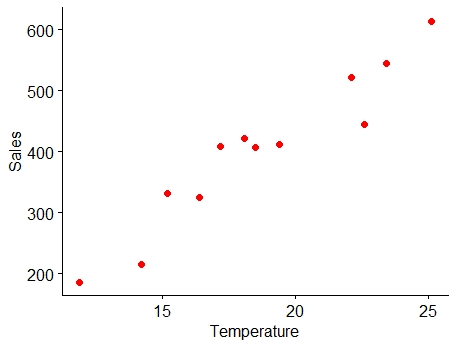
\includegraphics[width=0.5\linewidth]{images/image3c} 

}

\caption{Scatter plot of Example 7.2}\label{fig:c2}
\end{figure}

From the Figure 7.2 above you can see a linear association between the two variables \emph{i}.\emph{e}.
between temperature and ice cream sales. It can be shown using a line as
below. It is clear that as temperature increases sales increases,
indicating a positive correlation.

\begin{figure}

{\centering 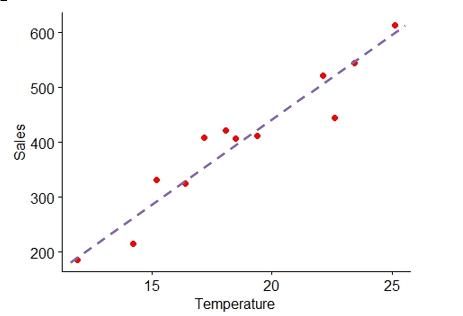
\includegraphics[width=0.5\linewidth]{images/image3.5c} 

}

\caption{Linear relationship between variables}\label{fig:c3}
\end{figure}

From the example it is clear that scatter diagram gives an idea on
linear association between variables, so it can also used as a graphical
tool to see whether there is correlation is present or not.

\begin{quote}
\textbf{Perfect Correlation}: If there is any change in the value of one
variable, the value of the other variable is changed in a fixed
proportion then the correlation between them is said to be a perfect
correlation. If there is a perfect correlation, the points will lie in
the straight line. In the scatter diagram of Example 7.2, you can see that
there is no perfect linear relationship as the points are not exactly in
the line, but the points are in some scattered form but still have a
direction (positive).
\end{quote}

Direction of correlation can be identified using a scatter diagram as shown below in Figure 7.4

\begin{figure}

{\centering 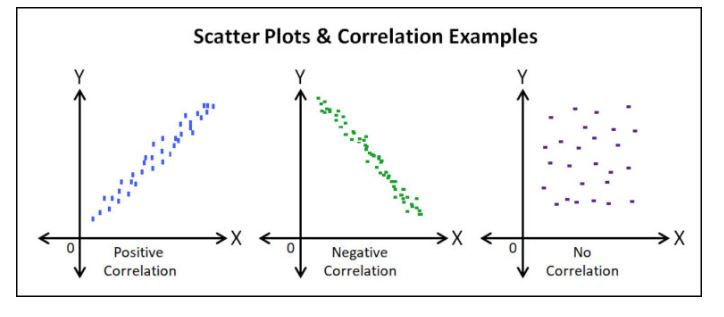
\includegraphics[width=0.7\linewidth]{images/image4c} 

}

\caption{Scatter plot and nature of relationship}\label{fig:c4}
\end{figure}

\hypertarget{karl-pearsons-coefficient-of-correlation-r}{%
\subsection{\texorpdfstring{Karl Pearson's coefficient of Correlation (\emph{r})}{Karl Pearson's coefficient of Correlation (r)}}\label{karl-pearsons-coefficient-of-correlation-r}}

It is the most important and widely used measure of correlation. A
measure of the intensity or degree of linear relationship between two
variables is developed by Karl Pearson, a British Biometrician - known
as the \textbf{\underline{Pearson's Correlation coefficient}} denoted by \textbf{\emph{r}}
which is expressed as the ratio of the \textbf{covariance} to the product of the standard deviations of the two variables.

\hypertarget{covariance}{%
\subsubsection{Covariance}\label{covariance}}

\textbf{Covariance} is a measure of the joint linear variability of the two
variables. Consider two variables \emph{x} and \emph{y} with \emph{n} observations
each, then covariance is given by the formula

Covariance of (\emph{x},\emph{y}) =
\(\frac{1}{n}\sum_{i = 1}^{n}{\left( x_{i} - \overline{x} \right)\left( y_{i} - \overline{y} \right)}\)

When covariance = 0 there is no joint variability or there is no linear
relationship. The unit of covariance is the product of the units of the
two variables.

Covariance of two variables \emph{x} and \emph{y} is denoted as \emph{Cov}(\emph{x}, \emph{y}).
Covariance measure is used to find correlation coefficient.

The correlation coefficient between the two variables (\emph{x} and \emph{y}) is
calculated as\\
\[r=\frac{cov(x,y)}{sd(x)sd(y)}\]

Where \emph{sd}. is the standard deviation.

\[r = \frac{\frac{1}{n}\sum_{i = 1}^{n}{\left( x_{i} - \overline{x} \right)\left( y_{i} - \overline{y} \right)}}{\sqrt{\frac{1}{n}\sum_{i = 1}^{n}\left( x_{i} - \overline{x} \right)^{2}\frac{1}{n}\sum_{i = 1}^{n}\left( y_{i} - \overline{y} \right)^{2}}}\]
\#\#\#\# Properties of the correlation coefficient (\emph{r})

\begin{enumerate}
\def\labelenumi{\arabic{enumi}.}
\item
  It is a pure number independent of both origin and scale of the
  units of the observations.
\item
  It always lies between −1 and +1 (absolute value cannot exceed
  unity). \textbf{−1} ≤ \emph{r} ≤ \textbf{+1}
\item
  \emph{r} = +1, indicates perfect positive correlation. \emph{r} = −1,
  indicates perfect negative correlation. \emph{r} = 0, indicates no
  correlation.
\item
  When the correlation is zero then there is no linear relationship
  between the variables.
\item
  If there is no meaningful relation between the variables the value
  of the correlation obtained is also meaningless. (For example as
  fertilizer price increases, Kohili's batting average also increases,
  we know there no practical relationship between these variables,
  still we may get a correlation measure and it is called \emph{spurious
  correlation})
\item
  A Simplified formula for computation of correlation coefficient can
  be derived by modifying above formula
\end{enumerate}

\[r = \frac{n\left( \sum_{i = 1}^{n}{x_{i}y_{i}} \right) - \sum_{i = 1}^{n}{x_{i}\sum_{i = 1}^{n}y_{i}}}{\sqrt{\left\lbrack n\sum_{i = 1}^{n}{x_{i}^{2} - \left( \sum_{i = 1}^{n}x_{i} \right)^{2}} \right\rbrack\left\lbrack n\sum_{i = 1}^{n}{y_{i}^{2} - \left( \sum_{i = 1}^{n}y_{i} \right)^{2}} \right\rbrack}}\]

\textbf{Example 7.3}: Consider the Example 7.2 of ice cream sales; find
correlation coefficient (\emph{r})

\begin{longtable}[]{@{}
  >{\raggedright\arraybackslash}p{(\columnwidth - 14\tabcolsep) * \real{0.12}}
  >{\raggedright\arraybackslash}p{(\columnwidth - 14\tabcolsep) * \real{0.18}}
  >{\raggedright\arraybackslash}p{(\columnwidth - 14\tabcolsep) * \real{0.09}}
  >{\raggedright\arraybackslash}p{(\columnwidth - 14\tabcolsep) * \real{0.11}}
  >{\raggedright\arraybackslash}p{(\columnwidth - 14\tabcolsep) * \real{0.12}}
  >{\raggedright\arraybackslash}p{(\columnwidth - 14\tabcolsep) * \real{0.12}}
  >{\raggedright\arraybackslash}p{(\columnwidth - 14\tabcolsep) * \real{0.12}}
  >{\raggedright\arraybackslash}p{(\columnwidth - 14\tabcolsep) * \real{0.14}}@{}}
\toprule
Sl. No. & Temperature & Sales & \(x_{i}-\overline{x}\)(1) & \(y_{i}-\overline{y}\)(2) & (1).(2) & \((x_{i}-\overline{x})^{2}\) & \((y_{i}-\overline{y})^{2}\) \\
\midrule
\endhead
& (x) & (y) & & & & & \\
1 & 14.2 & 215 & -4.475 & -187.42 & 838.69 & 20.0256 & 35125.01 \\
2 & 16.4 & 325 & -2.275 & -77.417 & 176.123 & 5.17563 & 5993.34 \\
3 & 11.9 & 185 & -6.775 & -217.42 & 1473 & 45.9006 & 47270.01 \\
4 & 15.2 & 332 & -3.475 & -70.417 & 244.698 & 12.0756 & 4958.507 \\
5 & 18.5 & 406 & -0.175 & 3.58333 & -0.6271 & 0.03063 & 12.84028 \\
6 & 22.1 & 522 & 3.425 & 119.583 & 409.573 & 11.7306 & 14300.17 \\
7 & 19.4 & 412 & 0.725 & 9.58333 & 6.94792 & 0.52562 & 91.84028 \\
8 & 25.1 & 614 & 6.425 & 211.583 & 1359.42 & 41.2806 & 44767.51 \\
9 & 23.4 & 544 & 4.725 & 141.583 & 668.981 & 22.3256 & 20045.84 \\
10 & 18.1 & 421 & -0.575 & 18.5833 & -10.685 & 0.33062 & 345.3403 \\
11 & 22.6 & 445 & 3.925 & 42.5833 & 167.14 & 15.4056 & 1813.34 \\
12 & 17.2 & 408 & -1.475 & 5.58333 & -8.2354 & 2.17563 & 31.17361 \\
\textbf{SUM} & \textbf{224.1} & \textbf{4829} & 0 & 0 & \textbf{5325.03} & \textbf{176.983} & \textbf{174754.9} \\
\bottomrule
\end{longtable}

\emph{n} =12

\[mean,\overline{x} = \ \frac{224.1}{12} = 18.675\]

\[mean,\overline{y} = \ \frac{4829}{12} = 402.416\]

\emph{Cov} (\emph{x},\emph{y}) =
\(\frac{1}{n}\sum_{i = 1}^{n}{\left( x_{i} - \overline{x} \right)\left( y_{i} - \overline{y} \right)}\)

\(\sum_{i = 1}^{12}{\left( x_{i} - \overline{x} \right)\left( y_{i} - \overline{y} \right)} = 5325.03\)

\emph{Cov} (\emph{x},\emph{y}) = \(\frac{5325.03}{12} = 443.752\)

\[Standard\ deviation,\ S.D\left( x \right) = \ \sqrt{\frac{1}{n}\sum_{i = 1}^{n}\left( x_{i} - \overline{x} \right)^{2}} = \sqrt{\frac{176.983}{12}} = 3.840\]

\[Standard\ deviation,\ S.D\left( y \right) = \ \sqrt{\frac{1}{n}\sum_{i = 1}^{n}\left( y_{i} - \overline{y} \right)^{2}} = \sqrt{\frac{174754.9}{12}} = 120.676\]

\(r = \frac{443.752}{3.840\  \times 120.676} = 0.95751\), which indicates
a strong positive correlation

\hypertarget{spearmans-rank-order-correlation-coefficient-ux3c1}{%
\subsection{\texorpdfstring{Spearman's Rank order correlation coefficient (\emph{ρ})}{Spearman's Rank order correlation coefficient (ρ)}}\label{spearmans-rank-order-correlation-coefficient-ux3c1}}

The Spearman correlation evaluates the monotonic relationship between
two continuous or ordinal variables.

Note: What is a monotonic relation?

In a monotonic relationship, the variables tend to move in the same
relative direction, but not necessarily at a constant rate. In a linear
relationship, the variables move in the same direction at a constant
rate.

Linear relationship is monotonic but all monotonic relations are not
linear. You can see the plots below for better understanding.

\begin{figure}

{\centering 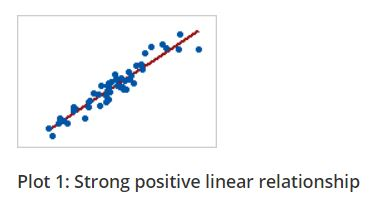
\includegraphics[width=0.49\linewidth]{images/image6c} 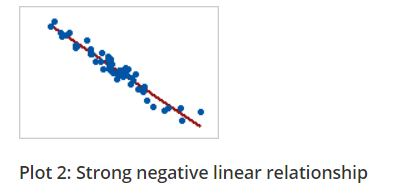
\includegraphics[width=0.49\linewidth]{images/image7c} 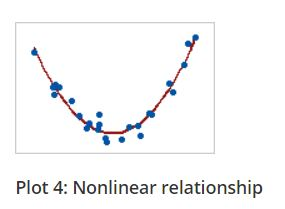
\includegraphics[width=0.49\linewidth]{images/image8c} 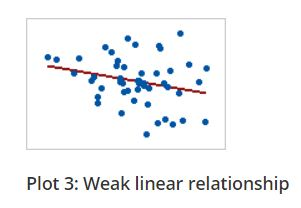
\includegraphics[width=0.49\linewidth]{images/image9c} 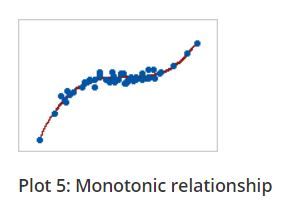
\includegraphics[width=0.49\linewidth]{images/image10c} 

}

\caption{Linear and Monotonic relationship}\label{fig:c6}
\end{figure}

The Spearman correlation coefficient is based on the ranked values for
each variable rather than the raw data. The spearman correlation
measures the monotonic relationship between variables, where pearsons
correlation coefficient measures linear relationship only. To use
Spearman's correlation coefficient your data must be in ordinal,
interval or ratio scale.

There are two cases in calculating \emph{ρ}. One is in case of no tied rank
other is when there is tied rank

\hypertarget{no-tied-rank-case}{%
\subsubsection{No tied rank case}\label{no-tied-rank-case}}

When two or more distinct observations have the same
value, thus being given the same rank, they are said to be tied

The formula for the Spearman rank correlation coefficient when there are
no tied ranks is:

\[\rho = 1 - \frac{6\sum_{i = 1}^{n}d_{i}^{2}}{n\left( n^{2} - 1 \right)}\]

Where \(d_{i}\) is the difference between ranks of \emph{i\textsuperscript{t}}\textsuperscript{h} pair of
observation

\textbf{Example 7.4}: Calculation of Spearman's rank correlation when there is
no tied rank is explained step by step by using the example below

The scores for nine students in physics and math are as follows:

Physics: 35, 23, 47, 17, 10, 43, 9, 6, 28

Mathematics: 30, 33, 45, 23, 8, 49, 12, 4, 31

Compute the student's ranks in the two subjects and compute the Spearman
rank correlation.

\begin{longtable}[]{@{}ll@{}}
\toprule
Physics & Mathematics \\
\midrule
\endhead
35 & 30 \\
23 & 33 \\
47 & 45 \\
17 & 23 \\
10 & 8 \\
43 & 49 \\
9 & 12 \\
6 & 4 \\
28 & 31 \\
\bottomrule
\end{longtable}

\textbf{Step 1}: Find the ranks for each individual subject. Rank the scores
from greatest to smallest; assign the rank 1 to the highest score, 2 to
the next highest and so on:

\begin{longtable}[]{@{}
  >{\raggedright\arraybackslash}p{(\columnwidth - 6\tabcolsep) * \real{0.22}}
  >{\raggedright\arraybackslash}p{(\columnwidth - 6\tabcolsep) * \real{0.10}}
  >{\raggedright\arraybackslash}p{(\columnwidth - 6\tabcolsep) * \real{0.19}}
  >{\raggedright\arraybackslash}p{(\columnwidth - 6\tabcolsep) * \real{0.10}}@{}}
\toprule
Physics (\emph{x}) & Rank & Mathematics

(\emph{y}) & Rank \\
\midrule
\endhead
35 & 3 & 30 & 5 \\
23 & 5 & 33 & 3 \\
47 & 1 & 45 & 2 \\
17 & 6 & 23 & 6 \\
10 & 7 & 8 & 8 \\
43 & 2 & 49 & 1 \\
9 & 8 & 12 & 7 \\
6 & 9 & 4 & 9 \\
28 & 4 & 31 & 4 \\
\bottomrule
\end{longtable}

\textbf{Step 2}: Add a column \emph{d}, to your data. The \emph{d} is the difference
between ranks. For example, the first student's physics rank is 3 and
math rank is 5, so the difference is -2. In the next column, square your
\emph{d} values.

\begin{longtable}[]{@{}
  >{\raggedright\arraybackslash}p{(\columnwidth - 10\tabcolsep) * \real{0.22}}
  >{\raggedright\arraybackslash}p{(\columnwidth - 10\tabcolsep) * \real{0.12}}
  >{\raggedright\arraybackslash}p{(\columnwidth - 10\tabcolsep) * \real{0.19}}
  >{\raggedright\arraybackslash}p{(\columnwidth - 10\tabcolsep) * \real{0.10}}
  >{\raggedright\arraybackslash}p{(\columnwidth - 10\tabcolsep) * \real{0.08}}
  >{\raggedright\arraybackslash}p{(\columnwidth - 10\tabcolsep) * \real{0.12}}@{}}
\toprule
Physics (\emph{x}) & Rank & Mathematics

(\emph{y}) & Rank & \emph{d} & \emph{d}\textsuperscript{2} \\
\midrule
\endhead
35 & 3 & 30 & 5 & -2 & 4 \\
23 & 5 & 33 & 3 & 2 & 4 \\
47 & 1 & 45 & 2 & -1 & 1 \\
17 & 6 & 23 & 6 & 0 & 0 \\
10 & 7 & 8 & 8 & -1 & 1 \\
43 & 2 & 49 & 1 & 1 & 1 \\
9 & 8 & 12 & 7 & 1 & 1 \\
6 & 9 & 4 & 9 & 0 & 0 \\
28 & 4 & 31 & 4 & 0 & 0 \\
\textbf{SUM} & \textbf{12} & & & & \\
\bottomrule
\end{longtable}

\textbf{Step 4}: Sum (add up) all of your \emph{d}\textsuperscript{2} values. 4 + 4 + 1 + 0 + 1 +
1 + 1 + 0 + 0 = 12. You'll need this for the formula (the
\(\sum_{i = 1}^{n}d_{i}^{2}\) is just ``the sum of \emph{d}\textsuperscript{2}values, here \emph{n}=
9'').

\textbf{Step 5}: Insert the values into the formula.

\[\rho = 1 - \frac{6\sum_{i = 1}^{n}d_{i}^{2}}{n\left( n^{2} - 1 \right)}\]

\[\rho = 1 - \frac{6 \times 12}{9\left( 81 - 1 \right)} = 0.90\]

The Spearman's Rank Correlation for this set of data is 0.9.

Spearman's Rank Correlation also lies between −1 and +1 always. −1 ≤ \emph{ρ}
≤+1

\hypertarget{tied-rank-case}{%
\subsubsection{Tied rank case}\label{tied-rank-case}}

Calculation of Spearman's rank correlation when there is
tied rank is explained step by step by using the example below

\textbf{Example 7.5}: The scores for nine students in physics and mathematics are as follows:

\begin{longtable}[]{@{}
  >{\raggedright\arraybackslash}p{(\columnwidth - 2\tabcolsep) * \real{0.14}}
  >{\raggedright\arraybackslash}p{(\columnwidth - 2\tabcolsep) * \real{0.19}}@{}}
\toprule
Physics

(\emph{x}) & Mathematics

(\emph{y}) \\
\midrule
\endhead
35 & 30 \\
23 & 33 \\
47 & 45 \\
23 & 23 \\
10 & 8 \\
43 & 49 \\
9 & 12 \\
6 & 33 \\
28 & 33 \\
\bottomrule
\end{longtable}

\textbf{Step 1}: Consider the marks in Physics, ranked as usual

\begin{longtable}[]{@{}
  >{\raggedright\arraybackslash}p{(\columnwidth - 2\tabcolsep) * \real{0.14}}
  >{\raggedright\arraybackslash}p{(\columnwidth - 2\tabcolsep) * \real{0.10}}@{}}
\toprule
Physics

(\emph{x}) & Rank \\
\midrule
\endhead
35 & 3 \\
23 & 5 \\
47 & 1 \\
23 & 6 \\
10 & 7 \\
43 & 2 \\
9 & 8 \\
6 & 9 \\
28 & 4 \\
\bottomrule
\end{longtable}

You can see the value 23 is repeated, so may have equal ranks, so the
average of two ranks 5 and 6 is given to both;
\(\left( \frac{5 + 6}{2} \right)\ \)= 5.5

\begin{longtable}[]{@{}
  >{\raggedright\arraybackslash}p{(\columnwidth - 2\tabcolsep) * \real{0.14}}
  >{\raggedright\arraybackslash}p{(\columnwidth - 2\tabcolsep) * \real{0.10}}@{}}
\toprule
Physics

(\emph{x}) & Rank \\
\midrule
\endhead
35 & 3 \\
23 & 5.5 \\
47 & 1 \\
23 & 5.5 \\
10 & 7 \\
43 & 2 \\
9 & 8 \\
6 & 9 \\
28 & 4 \\
\bottomrule
\end{longtable}

Similarly for marks in mathematics you can see 33 is repeated thrice.

\begin{longtable}[]{@{}
  >{\raggedright\arraybackslash}p{(\columnwidth - 0\tabcolsep) * \real{0.19}}@{}}
\toprule
Mathematics

(\emph{y}) \\
\midrule
\endhead
30 \\
33 \\
45 \\
23 \\
8 \\
49 \\
12 \\
33 \\
33 \\
\bottomrule
\end{longtable}

\begin{longtable}[]{@{}
  >{\raggedright\arraybackslash}p{(\columnwidth - 2\tabcolsep) * \real{0.19}}
  >{\raggedright\arraybackslash}p{(\columnwidth - 2\tabcolsep) * \real{0.10}}@{}}
\toprule
Mathematics

(\emph{y}) & Rank \\
\midrule
\endhead
30 & 6 \\
33 & 3 \\
45 & 2 \\
23 & 7 \\
8 & 9 \\
49 & 1 \\
12 & 8 \\
33 & 4 \\
33 & 5 \\
\bottomrule
\end{longtable}

You can see the value 33 is repeated thrice, so the average of three
ranks 3, 4 and 5 is given \(\left( \frac{3 + 4 + 5}{3} \right)\ \)= 4

\begin{longtable}[]{@{}
  >{\raggedright\arraybackslash}p{(\columnwidth - 2\tabcolsep) * \real{0.19}}
  >{\raggedright\arraybackslash}p{(\columnwidth - 2\tabcolsep) * \real{0.10}}@{}}
\toprule
Mathematics

(\emph{y}) & Rank \\
\midrule
\endhead
30 & 6 \\
33 & 4 \\
45 & 2 \\
23 & 7 \\
8 & 9 \\
49 & 1 \\
12 & 8 \\
33 & 4 \\
33 & 4 \\
\bottomrule
\end{longtable}

\textbf{Step 2}: Change in the formula

\[\rho = 1 - \frac{6\left( \sum_{i = 1}^{n}d_{i}^{2} + T_{x} + T_{y} \right)}{n\left( n^{2} - 1 \right)}\]

If there are \emph{m} individuals tied (having same rank), and \emph{s} such sets
of ranks are there in X- series then,
\(T_{x} = \ \frac{1}{12}\sum_{i = 1}^{s}{m_{i}\left( m_{i}^{2} - 1 \right)}\)

In our example marks in Physics (\emph{x}) there are two 23 values tied
therefore \emph{m} = 2; since only one such a set is there \emph{s} =1

\(T_{x} = \ \frac{1}{12}\left( 2 \times (2^{2} - 1 \right)\) = 0.5

If there are \emph{w} individuals tied (having same rank), and \emph{s'} such sets
of ranks are there in Y- series then,
\(T_{y} = \ \frac{1}{12}\sum_{i = 1}^{s'}{w_{i}\left( w_{i}^{2} - 1 \right)}\)

In our example marks in Mathematics (\emph{y}) there are three 33 values tied
therefore \emph{w} = 3; since only one such a set is there \emph{s} =1

\(T_{y} = \ \frac{1}{12}\left( 3 \times (3^{2} - 1 \right)\) = 2

\textbf{Step 2}: Calculate \emph{d} and then use the formula

\begin{longtable}[]{@{}
  >{\raggedright\arraybackslash}p{(\columnwidth - 10\tabcolsep) * \real{0.14}}
  >{\raggedright\arraybackslash}p{(\columnwidth - 10\tabcolsep) * \real{0.10}}
  >{\raggedright\arraybackslash}p{(\columnwidth - 10\tabcolsep) * \real{0.19}}
  >{\raggedright\arraybackslash}p{(\columnwidth - 10\tabcolsep) * \real{0.10}}
  >{\raggedright\arraybackslash}p{(\columnwidth - 10\tabcolsep) * \real{0.10}}
  >{\raggedright\arraybackslash}p{(\columnwidth - 10\tabcolsep) * \real{0.12}}@{}}
\toprule
Physics

(\emph{x}) & Rank & Mathematics

(\emph{y}) & Rank & \emph{d} & \emph{d}\textsuperscript{2} \\
\midrule
\endhead
35 & 3 & 30 & 6 & -3 & 9 \\
23 & 5.5 & 33 & 4 & 1.5 & 2.25 \\
47 & 1 & 45 & 2 & -1 & 1 \\
23 & 5.5 & 23 & 7 & -1.5 & 2.25 \\
10 & 7 & 8 & 9 & -2 & 4 \\
43 & 2 & 49 & 1 & 1 & 1 \\
9 & 8 & 12 & 8 & 0 & 0 \\
6 & 9 & 33 & 4 & 5 & 25 \\
28 & 4 & 33 & 4 & 0 & 0 \\
SUM & 0 & 44.5 & & & \\
\bottomrule
\end{longtable}

\(\rho = 1 - \frac{6\left( \sum_{i = 1}^{n}d_{i}^{2} + T_{x} + T_{y} \right)}{n\left( n^{2} - 1 \right)} = 1 - \frac{6 \times \left( 44.5 + 0.5 + 2 \right)}{9\left( 9^{2} - 1 \right)} = \ 1 - \frac{282}{720}\)
= 0.60834

\hypertarget{kendalls-rank-correlation-coefficient-ux3c4}{%
\subsection{\texorpdfstring{Kendall's Rank Correlation Coefficient (\emph{τ})}{Kendall's Rank Correlation Coefficient (τ)}}\label{kendalls-rank-correlation-coefficient-ux3c4}}

Kendall's rank correlation coefficient also known as Kendall's Tau or
coefficient of concordance. It lies between 0 and 1, 0 ≤ \emph{τ ≤} 1. when
several sets of ranks are there, it can be used to test the association.

When we have \emph{k} sets of rankings we may determine the association among
them by using the Kendall's coefficient of Concordance (\emph{τ}). Such a
measure is useful to study the reliability in the scorings made by a
number of Judges.

Arrange the data into a table with each row representing the ranks
assigned by (each judge), to say, \emph{n} number of objects. Let there be
\emph{k} number of sets of rankings for each object given by \emph{k} judges. Then
the Kendall's coefficient of concordance \emph{τ} is computed as

\[\tau = \frac{12\left\lbrack \sum_{i = 1}^{n}{R_{i}^{2} - \frac{\left( \sum_{i = 1}^{n}R_{i} \right)^{2}}{n}} \right\rbrack}{k^{2}n\left( n^{2} - 1 \right)}\]

\textbf{Example 7.6}: In a crop production competition, 10 entries of farmers
were ranked by agricultural scientists (judges). Find the degree of
agreement among the scientist for the competition result given below.

\begin{longtable}[]{@{}lllll@{}}
\toprule
& Ranks given by the judges to farmers & & & \\
\midrule
\endhead
Farmers & Scientist 1 & Scientist 2 & Scientist 3 & Scientist 4 \\
1 & 4 & 5 & 3 & 7 \\
2 & 10 & 9 & 8 & 6 \\
3 & 8 & 6 & 10 & 9 \\
4 & 3 & 4 & 2 & 1 \\
5 & 1 & 3 & 4 & 2 \\
6 & 2 & 1 & 1 & 4 \\
7 & 5 & 7 & 6 & 5 \\
8 & 6 & 2 & 5 & 3 \\
9 & 7 & 8 & 9 & 10 \\
10 & 9 & 10 & 7 & 8 \\
\bottomrule
\end{longtable}

Solution:

\begin{longtable}[]{@{}lllllll@{}}
\toprule
Farmers & S1 & S2 & S3 & S4 & \(R_{i}\) (sum of ranks) & \(R_{i}^{2}\) \\
\midrule
\endhead
1 & 4 & 5 & 3 & 7 & 19 & 361 \\
2 & 10 & 9 & 8 & 6 & 33 & 1089 \\
3 & 8 & 6 & 10 & 9 & 33 & 1089 \\
4 & 3 & 4 & 2 & 1 & 10 & 100 \\
5 & 1 & 3 & 4 & 2 & 10 & 100 \\
6 & 2 & 1 & 1 & 4 & 8 & 64 \\
7 & 5 & 7 & 6 & 5 & 23 & 529 \\
8 & 6 & 2 & 5 & 3 & 16 & 256 \\
9 & 7 & 8 & 9 & 10 & 34 & 1156 \\
10 & 9 & 10 & 7 & 8 & 34 & 1156 \\
\textbf{SUM} & 220 & 5900 & & & & \\
\bottomrule
\end{longtable}

Here \emph{k} = number of judges = 4

\emph{n} = number of farmers =10

\(\left( \sum_{i = 1}^{10}R_{i} \right)^{2}\ \)= (220)\textsuperscript{2} = 48400

\(\sum_{i = 1}^{10}R_{i}^{2}\) = 5900

\[\tau = \frac{12\left\lbrack \sum_{i = 1}^{n}{R_{i}^{2} - \frac{\left( \sum_{i = 1}^{n}R_{i} \right)^{2}}{n}} \right\rbrack}{k^{2}n\left( n^{2} - 1 \right)}\]

=\\
\(\tau = \frac{12\left\lbrack 5900 - \frac{48400}{10} \right\rbrack}{16 \times 10\left( 100 - 1 \right)}\)
= 0.803

Since \(\tau\) is nearly equal to 1, the ranks given by judges were almost
same

*************************************************

\hypertarget{regression-analysis}{%
\chapter{Regression Analysis}\label{regression-analysis}}

Regression analysis is the method of using observations (data records)
to quantify the relationship between a target variable also referred to
as a \emph{dependent variable}, and a set of \emph{independent variables}.

\hypertarget{definition}{%
\section{Definition}\label{definition}}

Regression analysis is a mathematical measure of the
average relationship between two or more variables in terms of the
original units of the data

\hypertarget{simple-regression}{%
\section{Simple regression}\label{simple-regression}}

when only two variables are involved; Regression
can be defined as the functional relationship between two variables,
where one may represent cause and the other may represent effect. The
variable representing cause is known as independent variable and is
denoted by `X'. The variable `X' is also known as predictor variable,
regressor or explanatory variable. The variable representing effect is
known as dependent variable and is denoted by Y. For example consider
yield and fertilizer dose, here yield can be considered as dependent
variable (Y) and fertilizer dose can be considered as independent
variable (X).

\hypertarget{two-types-of-variables}{%
\section{Two types of variables}\label{two-types-of-variables}}

In regression analysis the
variable whose values need to be predicted (Y) is called \textbf{dependent variable} and the variable which is used for prediction (X) is called
\textbf{independent variable.}

When more than two independent variables are present then the regression
is called as \textbf{Multiple Regression}. If only two variables are present
then it is called as \textbf{simple regression}.

\hypertarget{detailed-explanation}{%
\section{Detailed explanation}\label{detailed-explanation}}

Correlation is a statistical measure which determines the degree of
association of two variables. Regression on other hand side describes
how an independent variable is numerically related to dependent
variable.

Regression can be simply defined as a technique of fitting best line or
line of best fit to estimate value of one variable on the basis of
another variable. Now what is a best line? or line of best fit?

For explaining further, consider the example of Ice cream sales:

\textbf{Example 8.1}: The local ice cream shop keeps track of how much ice
cream they sell versus the temperature on that day; here are their
figures for the last 12 days:

\begin{longtable}[]{@{}ll@{}}
\toprule
Temperature (°C) & Ice Cream Sales (in \$) \\
\midrule
\endhead
14.2 & 215 \\
16.4 & 325 \\
11.9 & 185 \\
15.2 & 332 \\
18.5 & 406 \\
22.1 & 522 \\
19.4 & 412 \\
25.1 & 614 \\
23.4 & 544 \\
18.1 & 421 \\
22.6 & 445 \\
17.2 & 408 \\
\bottomrule
\end{longtable}

We can use regression analysis to answer the following questions

What will be the Ice cream sales when temperature is 20\textsuperscript{o} Celsius?

What is the functional form of relationship between Temperature and Ice
cream sales?

\begin{figure}

{\centering 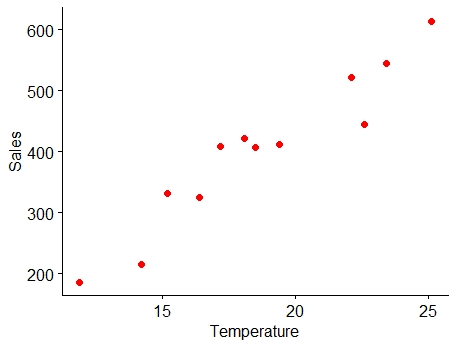
\includegraphics[width=0.5\linewidth]{images/r2} 

}

\caption{Scatter diagram of data in Example 8.1}\label{fig:r1}
\end{figure}

We can draw a line to denote the functional relationship between temperature and sales

\begin{figure}

{\centering 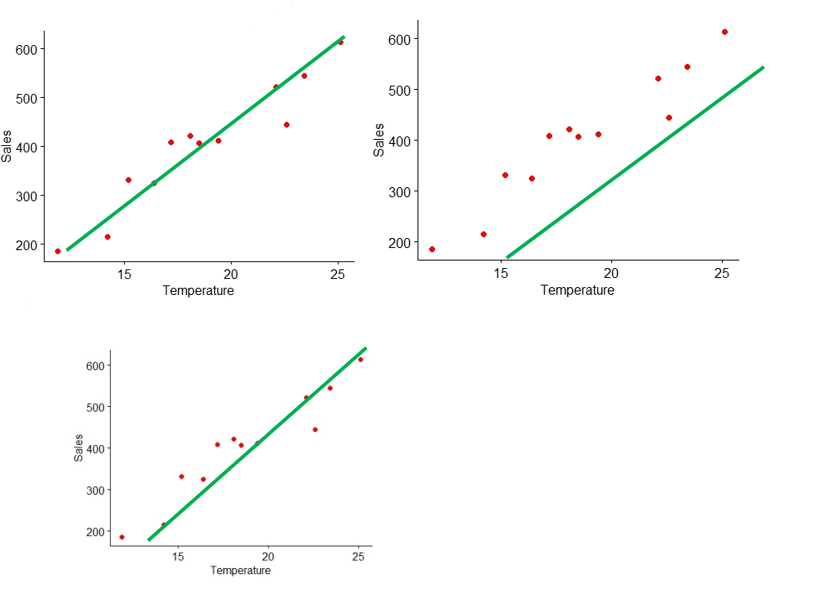
\includegraphics[width=0.5\linewidth]{images/r99} 

}

\caption{lines drawn to show functional relationship}\label{fig:r2}
\end{figure}

You can see that as shown above we can draw any number of lines, so
which is the best fit line?

We can say the \textbf{best fit line} is the line that passes through all
points such that distance of each point to the line is minimum. Using
regression technique we could easily draw such a line. Before proceeding
you should know the concept of error and residuals.

\hypertarget{error-and-residual}{%
\section{Error and residual}\label{error-and-residual}}

An error is the difference between the observed value and the true value
(true value is the unobserved population mean of the population from
which sample observations are taken). A residual is the difference
between the observed value and the predicted value (by the model
{[}fitted line{]}). Error cannot be measured but residual can be; so
residual is considered as an estimate of error.

\begin{figure}

{\centering 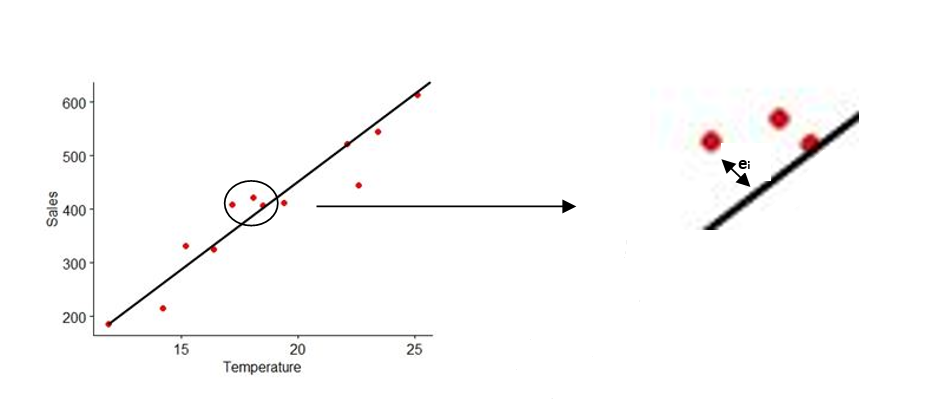
\includegraphics[width=0.5\linewidth]{images/r91} 

}

\caption{Error depicted in best fit line }\label{fig:r3}
\end{figure}

The distance of each observation (\emph{e}\textsubscript{i}) from the fitted line can be
considered as the residual (error). Best fit line can be obtained by
minimizing this distance. This can be achieved using the mathematical
technique ``\textbf{principle of least squares}''.

\hypertarget{straight-lines}{%
\section{Straight lines}\label{straight-lines}}

A straight line is the simplest figure in geometry.

Mathematical equation of a straight line Y= \textbf{\emph{a}} + \textbf{\emph{b}}X.

Two important features of a line \textbf{slope} and \textbf{intercept}. \textbf{\emph{a}} is
the Y-intercept, the intercept of a line is the y-value of the point
where it crosses the y-axis. \textbf{\emph{b}} is the \textbf{slope of a line,} which
is a number that measures its "steepness. It is the change in Y for a
unit change in X along the line. In regression \textbf{\emph{b}} is called as
regression coefficient

Intercept (\textbf{\emph{a}})

\begin{figure}

{\centering 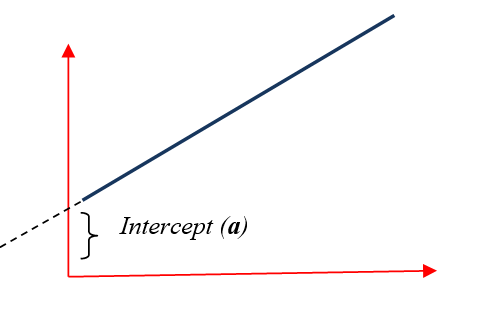
\includegraphics[width=0.5\linewidth]{images/r92} 

}

\caption{Intercept of a line }\label{fig:r4}
\end{figure}

Slope (\textbf{\emph{b}})

\begin{figure}

{\centering 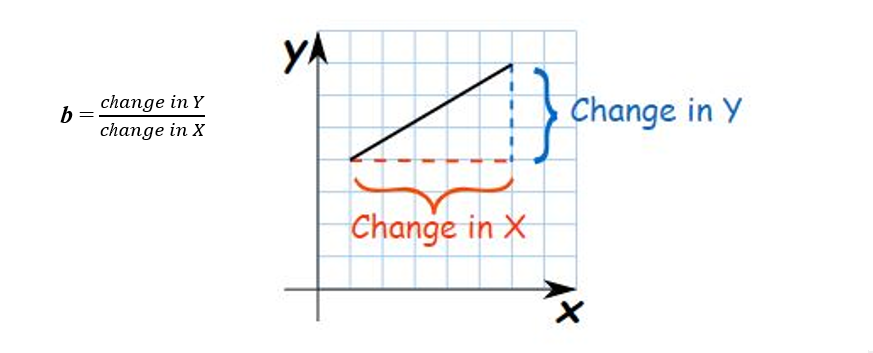
\includegraphics[width=0.5\linewidth]{images/r93} 

}

\caption{Slope of a line }\label{fig:r5}
\end{figure}

\textbf{\emph{a}} and \textbf{\emph{b}} can be considered as a finger print of a line; with
these values we can easily identify the line.

So now our problem is simple, to find a line of best, estimate \textbf{\emph{a}} \&
\textbf{\emph{b}}, such that error \emph{e}\textsubscript{i} of each observation is minimized. For
that we use the \textbf{method of least squares}.

\hypertarget{method-of-least-squares}{%
\section{Method of least squares}\label{method-of-least-squares}}

On considering the error term \emph{e}\textsubscript{i}; equation of a straight line is

\emph{y}\textsubscript{i}=\emph{a}+\emph{bx}\textsubscript{i}+\emph{e\textsubscript{i}};

Where \emph{e\textsubscript{i}} is the \emph{i}\textsuperscript{th} error term corresponding to \emph{y}\textsubscript{i}, \emph{i}
=1,2,...,\emph{n}

Line of best fit can be obtained by estimating \textbf{\emph{a}} and \textbf{\emph{b}} by
minimizing error sum 'Σ\emph{e\textsubscript{i}'}. By theorem Σ\emph{e\textsubscript{i} =}0; so \textbf{\emph{a}} and
\textbf{\emph{b}} are estimated by minimising Σ\emph{e\textsubscript{i}} \textsuperscript{2}

\hypertarget{principle-of-least-squares}{%
\section{Principle of least squares}\label{principle-of-least-squares}}

The statistical method used to determine
a line of best fit by minimizing the~sum of squares of the error term
Σ\emph{e\textsubscript{i}} \textsuperscript{2}

\emph{y\textsubscript{i}}=\emph{a}+\emph{bx}\textsubscript{i}+\emph{e\textsubscript{i}};

\emph{e\textsubscript{i} =} \emph{y}\textsubscript{i} -- (\emph{a}+\emph{bx}\textsubscript{i})

\emph{e\textsubscript{i}}\textsuperscript{2} = \{\emph{y}\textsubscript{i} -- (\emph{a}+\emph{bx}\textsubscript{i})\}\textsuperscript{2}

\textbf{Σ} \emph{e\textsubscript{i}}\textsuperscript{2} = \textbf{Σ} \{\emph{y}\textsubscript{i} -- (\emph{a}+\emph{bx}\textsubscript{i})\}\textsuperscript{2}

\textbf{Σ} \emph{e\textsubscript{i}}\textsuperscript{2} is called as error sum of squares. As we are minimizing
error sum of squares, hence the name principle of least squares.

We want to minimize, \textbf{E = Σ} \emph{e}\textsubscript{i}\textsuperscript{2} = \textbf{Σ} \{\emph{y}\textsubscript{i} --
(\emph{a}+\emph{bx}\textsubscript{i})\}\textsuperscript{2}

\emph{i}.\emph{e}. we need to find \textbf{\emph{a}} and \textbf{\emph{b}} such that \textbf{E} is minimum

\textbf{E} can be minimized by taking derivative with respect to \textbf{\emph{a}} and
\textbf{\emph{b}} and equating to zero. On doing so we will get two equations,
these equations are termed as \textbf{normal equations} and solving those
normal equations will give the formula for \textbf{\emph{a}} and \textbf{\emph{b}}.

We are not discussing calculation part here. After taking derivatives we
will get two equations (Normal equations) as below:

\[\sum_{i = 1}^{n}{y_{i} = n\mathbf{a} + \mathbf{b}\sum_{i = 1}^{n}x_{i}}\]

\[\sum_{i = 1}^{n}{y_{i}x_{i} = \mathbf{a}\sum_{i = 1}^{n}x_{i} + \mathbf{b}\sum_{i = 1}^{n}x_{i}^{2}}\]

On solving the above equations we will get

Regression coefficient, \textbf{\emph{b}} =
\(\frac{\sum_{i = 1}^{n}{y_{i}x_{i} - \frac{\sum_{i = 1}^{n}{y_{i}\sum_{i = 1}^{n}x_{i}}}{n}}}{\sum_{i = 1}^{n}x_{i}^{2} - \frac{\left( \sum_{i = 1}^{n}x_{i} \right)^{2}}{n}}\)

=\(\frac{cov(x,y)}{var(x)}\)

\[\mathbf{b =}\frac{\mathbf{cov(x,y)}}{\mathbf{var(x)}}
\]

\[\mathbf{a =}\overline{\mathbf{y}}\mathbf{- b}\overline{\mathbf{x}}\]

where \(\overline{y}\) = mean of \emph{y}; \(\overline{x}\) = mean of \emph{x}

\hypertarget{two-lines-of-regression}{%
\section{Two lines of regression}\label{two-lines-of-regression}}

There are two lines of regression- that of \emph{y} on \emph{x} and \emph{x} on \emph{y}.

\underline{Regression of \emph{y} on \emph{x}}

Consider the two variables \emph{x} and \emph{y}, if you are considering \emph{y} as
dependent variable and \emph{x} as independent variable then your equation
is:

\textbf{\emph{y} = \emph{a} + \emph{bx}}

This is used to predict the unknown value of variable \emph{y} when value of
variable \emph{x} is known. Usually \textbf{\emph{b}} here is denoted as \textbf{\emph{b}}\textsubscript{yx}

\[\mathbf{b}_{\mathbf{\text{yx}}}\mathbf{=}\frac{\mathbf{cov(x,y)}}{\mathbf{var(x)}}\]

Consider Example 8.1; considering ice cream sales as dependent variable
and temperature as independent variable

\begin{figure}

{\centering 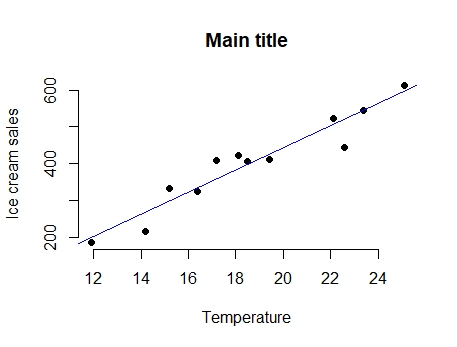
\includegraphics[width=0.5\linewidth]{images/r7} 

}

\caption{Scatter diagram of data in Example 8.1}\label{fig:r6}
\end{figure}

\underline{Regression of \emph{x} on \emph{y}}

Consider the two variables \emph{x} and \emph{y}, if you are considering \emph{x} as
dependent variable and \emph{y} as independent variable then your equation
is:

\textbf{\emph{x}= \emph{c} + \emph{my; }}where \textbf{\emph{c}} is the intercept and \textbf{\emph{m}} is the
slope

This is used to predict the unknown value of variable \emph{x} when value of
variable \emph{y} is known. Usually \textbf{\emph{b}} here is denoted as \textbf{\emph{b}}\textsubscript{xy}

\[\mathbf{b}_{\mathbf{\text{xy}}}\mathbf{=}\frac{\mathbf{cov(x,y)}}{\mathbf{var(y)}}\]

Consider Example 8.1; considering temperature as dependent variable and
ice cream sales as independent variable

\begin{figure}

{\centering 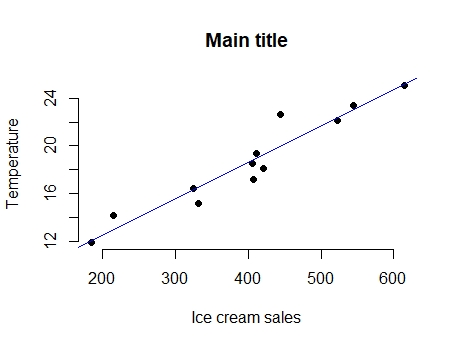
\includegraphics[width=0.5\linewidth]{images/r8} 

}

\caption{Scatter diagram of data in Example 8.1}\label{fig:r7}
\end{figure}

You can see both the regression were different. It depends on the
experimenter to choose dependent and independent variable. In the above
example it is evident that considering temperature as dependent variable
is meaningless, \emph{i}.\emph{e}. what is the usefulness in predicting
temperature based on ice cream sales?. So the selection of dependent and
independent variable is entirely the discretion of experimenter based on
the objective of his study.

\hypertarget{assumptions-of-regression}{%
\section{Assumptions of Regression}\label{assumptions-of-regression}}

If \emph{y} is the dependent variable and \emph{x} is the independent variable
then

\begin{enumerate}
\def\labelenumi{\arabic{enumi}.}
\item
  The \emph{x}'s are non-random or fixed constants
\item
  At each fixed value of \emph{x} the corresponding values of \emph{y} have a
  normal distribution about a mean.
\item
  For any given \emph{x}, the variance of \emph{y} is same.
\item
  The values of \emph{y} observed at different levels of \emph{x} are completely
  independent.
\end{enumerate}

\hypertarget{properties-of-regression-coefficients}{%
\section{Properties of Regression coefficients}\label{properties-of-regression-coefficients}}

\begin{enumerate}
\def\labelenumi{\arabic{enumi}.}
\tightlist
\item
  The correlation coefficient between \emph{x} and \emph{y} is the geometric
  mean of the two regression coefficients \textbf{\emph{b}}\textsubscript{yx} and \textbf{\emph{b}}\textsubscript{xy}
\end{enumerate}

\[r = \sqrt{b_{\text{yx}}b_{\text{xy}}}\]

\begin{enumerate}
\def\labelenumi{\arabic{enumi}.}
\setcounter{enumi}{1}
\item
  Regression coefficients are independent of change of origin but not
  of scale.
\item
  If one regression coefficient is greater than unit, then the other
  must be less than unit but not vice versa. \emph{i}.\emph{e}. both the
  regression coefficients can be less than unity but both cannot be
  greater than unity, \emph{i}.\emph{e}. if \textbf{\emph{b}}\textsubscript{yx} \textgreater1 then \textbf{\emph{b}}\textsubscript{xy} \textless1
  and if \textbf{\emph{b}}\textsubscript{xy} \textgreater1, then \textbf{\emph{b}}\textsubscript{yx} \textless1.
\item
  Also if one regression coefficient is positive the other must be
  positive (in this case the correlation coefficient is positive) and
  if one regression coefficient is negative the other must be negative
  (in this case the correlation coefficient is negative).
\end{enumerate}

\hypertarget{uses-of-regression}{%
\section{Uses of Regression}\label{uses-of-regression}}

\textbf{Prediction}: The regression analysis is useful in predicting the
value of one variable from the given value of another variable. Such
predictions are useful when it is very difficult or expensive to measure
the dependent variable, Y.

\textbf{Identify the strength of relationship}: the regression might be used
to identify the strength of the effect that the independent variable(s)
have on a dependent variable. Like the strength of relationship between
dose and effect, sales and marketing spending, or age and income.

\textbf{Forecast effects or impact of changes}: That is, the regression
analysis helps us to understand how much the dependent variable changes
with a change in one or more independent variables. A typical question
is, "how much additional sales income do I get for each additional 1000
spent on marketing

\textbf{Predicts trends and future values}: The regression analysis can be
used to predict trend and future values, like ``what will the price of
gold be in 6 months?''

\hypertarget{example-problem}{%
\section{Example problem}\label{example-problem}}

Now consider the example 8.1 and answer the questions

\begin{longtable}[]{@{}ll@{}}
\toprule
Temperature (°C) & Ice Cream Sales (in \$) \\
\midrule
\endhead
14.2 & 215 \\
16.4 & 325 \\
11.9 & 185 \\
15.2 & 332 \\
18.5 & 406 \\
22.1 & 522 \\
19.4 & 412 \\
25.1 & 614 \\
23.4 & 544 \\
18.1 & 421 \\
22.6 & 445 \\
17.2 & 408 \\
\bottomrule
\end{longtable}

\begin{enumerate}
\def\labelenumi{\arabic{enumi}.}
\item
  What is the functional form of relationship between Temperature and
  Ice cream sales?
\item
  What will be the Ice cream sales when temperature is 20\textsuperscript{o} Celsius?
\end{enumerate}

\textbf{Solution}

\begin{enumerate}
\def\labelenumi{\arabic{enumi}.}
\item
  Fit a model considering Ice cream sales as dependent variable (\emph{y})
  and temperature as independent variable (\emph{x}). Fitting a model means
  estimating \textbf{\emph{b}} and \textbf{\emph{a}} using equation.
\item
  After fitting the model put 20 in the \emph{x} value you will get the
  predicted \emph{y} value
\end{enumerate}

Model: \emph{y} = \textbf{\emph{a}}+\emph{\textbf{b}x}

\begin{longtable}[]{@{}
  >{\raggedright\arraybackslash}p{(\columnwidth - 6\tabcolsep) * \real{0.13}}
  >{\raggedright\arraybackslash}p{(\columnwidth - 6\tabcolsep) * \real{0.18}}
  >{\raggedright\arraybackslash}p{(\columnwidth - 6\tabcolsep) * \real{0.14}}
  >{\raggedright\arraybackslash}p{(\columnwidth - 6\tabcolsep) * \real{0.55}}@{}}
\toprule
Sl. No. & Temperature

(\emph{x}) & Sales

(\emph{y}) & \(x_{i} - \overline{x}\) \\
\midrule
\endhead
1 & 14.2 & 215 & -4.475 \\
2 & 16.4 & 325 & -2.275 \\
3 & 11.9 & 185 & -6.775 \\
4 & 15.2 & 332 & -3.475 \\
5 & 18.5 & 406 & -0.175 \\
6 & 22.1 & 522 & 3.425 \\
7 & 19.4 & 412 & 0.725 \\
8 & 25.1 & 614 & 6.425 \\
9 & 23.4 & 544 & 4.725 \\
10 & 18.1 & 421 & -0.575 \\
11 & 22.6 & 445 & 3.925 \\
12 & 17.2 & 408 & -1.475 \\
\textbf{SUM} & \textbf{224.1} & \textbf{4829} & \textbf{0} \\
\bottomrule
\end{longtable}

\begin{longtable}[]{@{}llll@{}}
\toprule
\(\left( y_{i} - \overline{y} \right)\) & \(\left( x_{i} - \overline{x} \right)\)× \(\left( y_{i} - \overline{y} \right)\) & \(\left( x_{i} - \overline{x} \right)^{2}\) & \(\left( y_{i} - \overline{y} \right)^{2}\) \\
\midrule
\endhead
-187.42 & 838.69 & 20.0256 & 35125.01 \\
-77.417 & 176.123 & 5.17563 & 5993.34 \\
-217.42 & 1473 & 45.9006 & 47270.01 \\
-70.417 & 244.698 & 12.0756 & 4958.507 \\
3.58333 & -0.6271 & 0.03063 & 12.84028 \\
119.583 & 409.573 & 11.7306 & 14300.17 \\
9.58333 & 6.94792 & 0.52562 & 91.84028 \\
211.583 & 1359.42 & 41.2806 & 44767.51 \\
141.583 & 668.981 & 22.3256 & 20045.84 \\
18.5833 & -10.685 & 0.33062 & 345.3403 \\
42.5833 & 167.14 & 15.4056 & 1813.34 \\
5.58333 & -8.2354 & 2.17563 & 31.17361 \\
\textbf{0} & \textbf{5325.03} & \textbf{176.983} & \textbf{174754.9} \\
\bottomrule
\end{longtable}

\emph{n} =12

\[mean,\overline{x} = \ \frac{224.1}{12} = 18.675\]

\[mean,\overline{y} = \ \frac{4829}{12} = 402.416\]

\emph{Cov} (\emph{x},\emph{y}) =
\(\frac{1}{n}\sum_{i = 1}^{n}{\left( x_{i} - \overline{x} \right)\left( y_{i} - \overline{y} \right)}\)

\(\sum_{i = 1}^{12}{\left( x_{i} - \overline{x} \right)\left( y_{i} - \overline{y} \right)} = 5325.03\)

\emph{Cov} (\emph{x},\emph{y}) = \(\frac{5325.03}{12} = 443.752\)

\[variance\ of\ x,\ var\left( x \right) = \ \frac{1}{n}\sum_{i = 1}^{n}\left( x_{i} - \overline{x} \right)^{2} = \frac{176.983}{12} = 14.7485\]

\[\mathbf{b =}\frac{\mathbf{cov(x,y)}}{\mathbf{var(x)}}\]

\[\mathbf{b =}\frac{443.752}{14.7485}\mathbf{=}30.088\]

\[\mathbf{a =}\overline{\mathbf{y}}\mathbf{- b}\overline{\mathbf{x}}\]

\[\mathbf{a =}402.416 - 30.088\left( 18.675 \right) = \  - 159.477\]

So our model is

\[y = \  - 159.477 + 30.088x\]

\[Ice\ cream\ sales = \  - 159.477 + 30.088(Temperature)\]

Ice cream sales when temperature is 20\textsuperscript{o} Celsius

\[x = 20\]

\(y = \  - 159.477 + 30.088(20)\) = 442.283

So the predicted ice cream sales at 20\textsuperscript{o} Celsius is \$442.283

**************************************************************

\hypertarget{references}{%
\chapter{References}\label{references}}

  \bibliography{book.bib}

\end{document}
